%% abtex2-modelo-trabalho-academico.tex, v-1.9.6 laurocesar
%% Copyright 2012-2016 by abnTeX2 group at http://www.abntex.net.br/ 
%%
%% This work may be distributed and/or modified under the
%% conditions of the LaTeX Project Public License, either version 1.3
%% of this license or (at your option) any later version.
%% The latest version of this license is in
%%   http://www.latex-project.org/lppl.txt
%% and version 1.3 or later is part of all distributions of LaTeX
%% version 2005/12/01 or later.
%%
%% This work has the LPPL maintenance status `maintained'.
%% 
%% The Current Maintainer of this work is the abnTeX2 team, led
%% by Lauro César Araujo. Further information are available on 
%% http://www.abntex.net.br/
%%
%% This work consists of the files abntex2-modelo-trabalho-academico.tex,
%% abntex2-modelo-include-comandos and abntex2-modelo-references.bib
%%

% ------------------------------------------------------------------------
% ------------------------------------------------------------------------
% abnTeX2: Modelo de Trabalho Academico (tese de doutorado, dissertacao de
% mestrado e trabalhos monograficos em geral) em conformidade com 
% ABNT NBR 14724:2011: Informacao e documentacao - Trabalhos academicos -
% Apresentacao
% ------------------------------------------------------------------------
% ------------------------------------------------------------------------

\documentclass[
	% -- opções da classe memoir --
	12pt,				% tamanho da fonte
	%openright,			% capítulos começam em pág ímpar (insere página vazia caso preciso)
	openany, %plinio custom	
	%twoside,			% para impressão em recto e verso. Oposto a oneside
	oneside, %plinio custom
	a4paper,			% tamanho do papel. 
	% -- opções da classe abntex2 --
	%chapter=TITLE,		% títulos de capítulos convertidos em letras maiúsculas
	%section=TITLE,		% títulos de seções convertidos em letras maiúsculas
	%subsection=TITLE,	% títulos de subseções convertidos em letras maiúsculas
	%subsubsection=TITLE,% títulos de subsubseções convertidos em letras maiúsculas
	% -- opções do pacote babel --
	english,			% idioma adicional para hifenização
	french,				% idioma adicional para hifenização
	spanish,			% idioma adicional para hifenização
	brazil				% o último idioma é o principal do documento
	]{abntex2}

% ---
% Pacotes básicos 
% ---
\usepackage{lmodern}			% Usa a fonte Latin Modern			
\usepackage[T1]{fontenc}		% Selecao de codigos de fonte.
\usepackage[utf8]{inputenc}		% Codificacao do documento (conversão automática dos acentos)
%\usepackage[latin1]{inputenc}
\usepackage{lastpage}			% Usado pela Ficha catalográfica
\usepackage{indentfirst}		% Indenta o primeiro parágrafo de cada seção.
\usepackage{color}				% Controle das cores
\usepackage{graphicx}			% Inclusão de gráficos
\usepackage{microtype} 			% para melhorias de justificação
\usepackage[export]{adjustbox}  % bordas em imagens
\usepackage{pdfpages}			%Plinio usou para incluir os PDF do apendice D
\usepackage{lscape}
\usepackage{float}
%\usepackage{chngcntr}

% ---
\counterwithin{figure}{chapter}
\counterwithin{table}{chapter}

%\counterwithout{figure}{section}
%\counterwithout{table}{section}
% ---
% Pacotes adicionais, usados apenas no âmbito do Modelo Canônico do abnteX2
% ---
\usepackage{lipsum}				% para geração de dummy text
% ---

% ---
% Pacotes de citações
% ---
\usepackage[brazilian,hyperpageref]{backref}	 % Paginas com as citações na bibl
\usepackage[alf]{abntex2cite}	% Citações padrão ABNT
\usepackage[table,xcdraw]{xcolor}
% --- 
% CONFIGURAÇÕES DE PACOTES
% --- 

% ---
% Configurações do pacote backref
% Usado sem a opção hyperpageref de backref
\renewcommand{\backrefpagesname}{Citado na(s) página(s):~}
% Texto padrão antes do número das páginas
\renewcommand{\backref}{}
% Define os textos da citação
\renewcommand*{\backrefalt}[4]{
	\ifcase #1 %
		Nenhuma citação no texto.%
	\or
		Citado na página #2.%
	\else
		Citado #1 vezes nas páginas #2.%
	\fi}%
% ---

% ---
% Informações de dados para CAPA e FOLHA DE ROSTO
% ---
%\titulo{Aplicando Grounded Theory para compreender as dificuldades de Planejamento de TI em Órgãos Federais}
\title{Uma Investigação sobre as Dificuldades de Planejamento de TI em Instituições Públicas Brasileiras: Uma Abordagem com Teoria Fundamentada em Dados}
\autor{Plínio Antunes Garcia}
\local{Recife, PE - Brasil}
\data{2016}
\orientador{Vinicius Cardoso Garcia}
%\coorientador{Equipe \abnTeX}
\instituicao{%
  Universidade Federal de Pernambuco - UFPE
  \par
  Centro de Informática - CIn
  \par
  Programa de Pós-Graduação em Ciência da Computação}
\tipotrabalho{Dissertação (Mestrado)}
% O preambulo deve conter o tipo do trabalho, o objetivo, 
% o nome da instituição e a área de concentração 
\preambulo{Este trabalho foi apresentado à Pós-Graduação em Ciência da
Computação do Centro de Informática da Universidade Federal de
Pernambuco como requisito parcial para obtenção do grau de Mestre.}
% ---


% ---
% Configurações de aparência do PDF final

% alterando o aspecto da cor azul
\definecolor{blue}{RGB}{41,5,195}

% informações do PDF
\makeatletter
\hypersetup{
     	%pagebackref=true,
		pdftitle={\@title}, 
		pdfauthor={\@author},
    	pdfsubject={\imprimirpreambulo},
	    pdfcreator={LaTeX with abnTeX2},
		pdfkeywords={abnt}{latex}{abntex}{abntex2}{trabalho acadêmico}, 
		colorlinks=true,       		% false: boxed links; true: colored links
    	linkcolor=blue,          	% color of internal links
    	citecolor=blue,        		% color of links to bibliography
    	filecolor=magenta,      		% color of file links
		urlcolor=blue,
		bookmarksdepth=4
}
\makeatother
% --- 

% --- 
% Espaçamentos entre linhas e parágrafos 
% --- 

% O tamanho do parágrafo é dado por:
\setlength{\parindent}{1.3cm}

% Controle do espaçamento entre um parágrafo e outro:
\setlength{\parskip}{0.2cm}  % tente também \onelineskip

% ---
% compila o indice
% ---
\makeindex
% ---

% ----
% Início do documento
% ----
\begin{document}

% Seleciona o idioma do documento (conforme pacotes do babel)
%\selectlanguage{english}
\selectlanguage{brazil}

% Retira espaço extra obsoleto entre as frases.
\frenchspacing 

% ----------------------------------------------------------
% ELEMENTOS PRÉ-TEXTUAIS
% ----------------------------------------------------------
% \pretextual

% ---
% Capa
% ---
%\imprimircapa
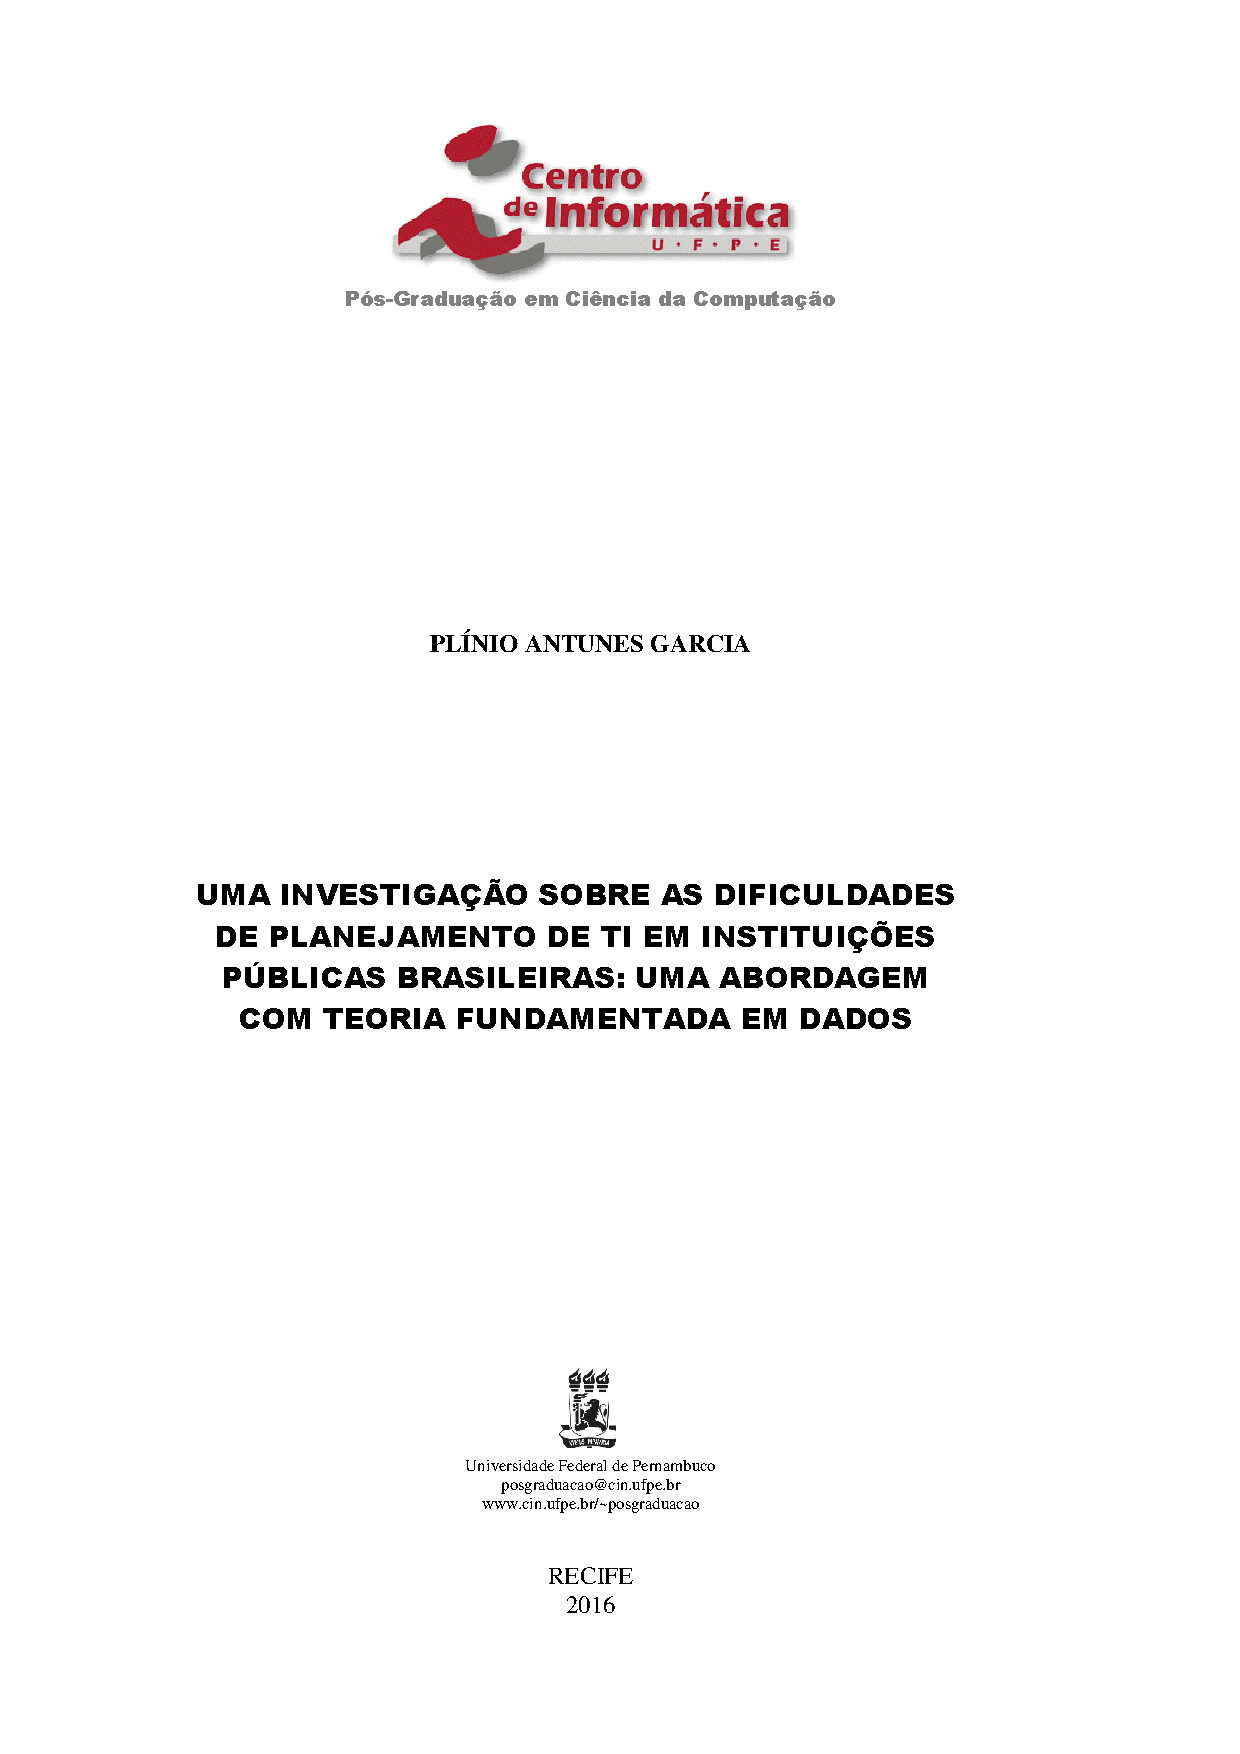
\includepdf[pages=-]{pre-textuais/capa.pdf}
% ---

% ---
% Folha de rosto
% (o * indica que haverá a ficha bibliográfica)
% ---
%\imprimirfolhaderosto*
%\imprimirfolhaderosto
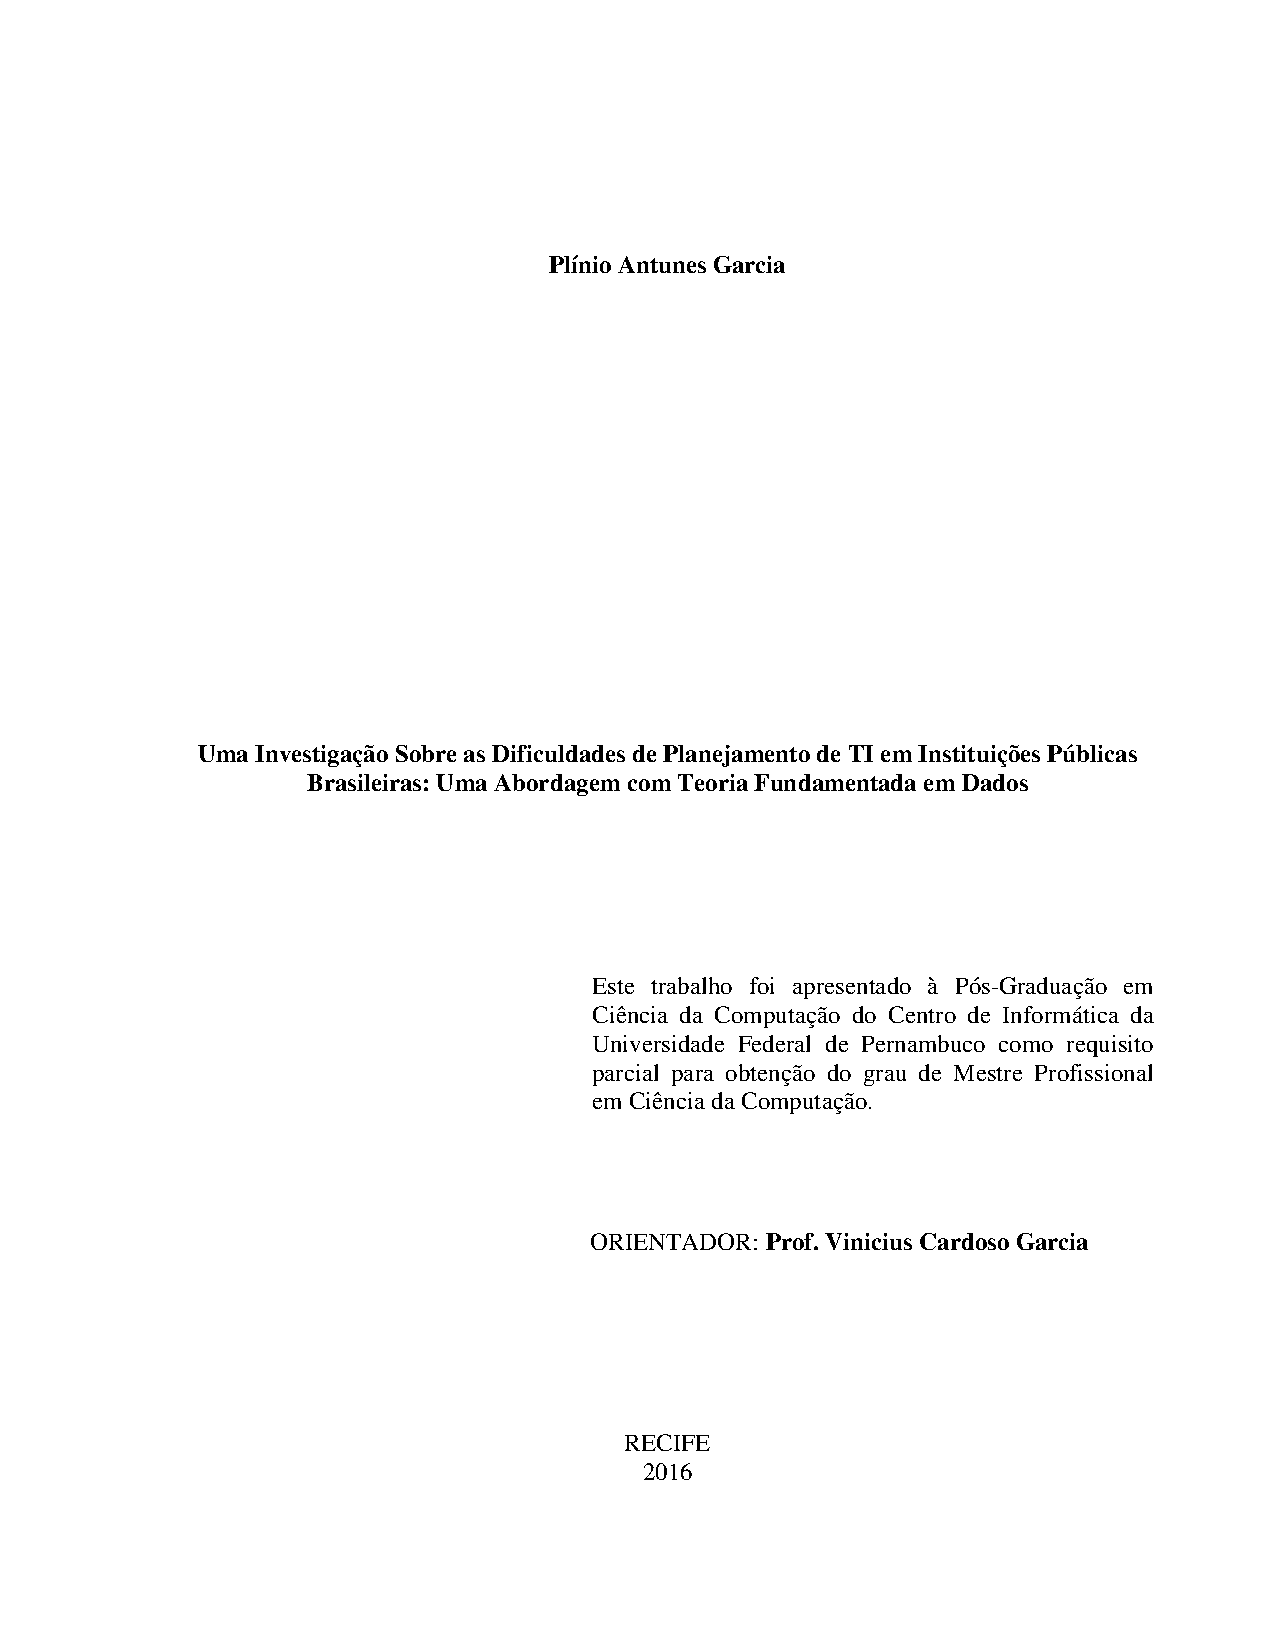
\includepdf[pages=-]{pre-textuais/folha_rosto.pdf}
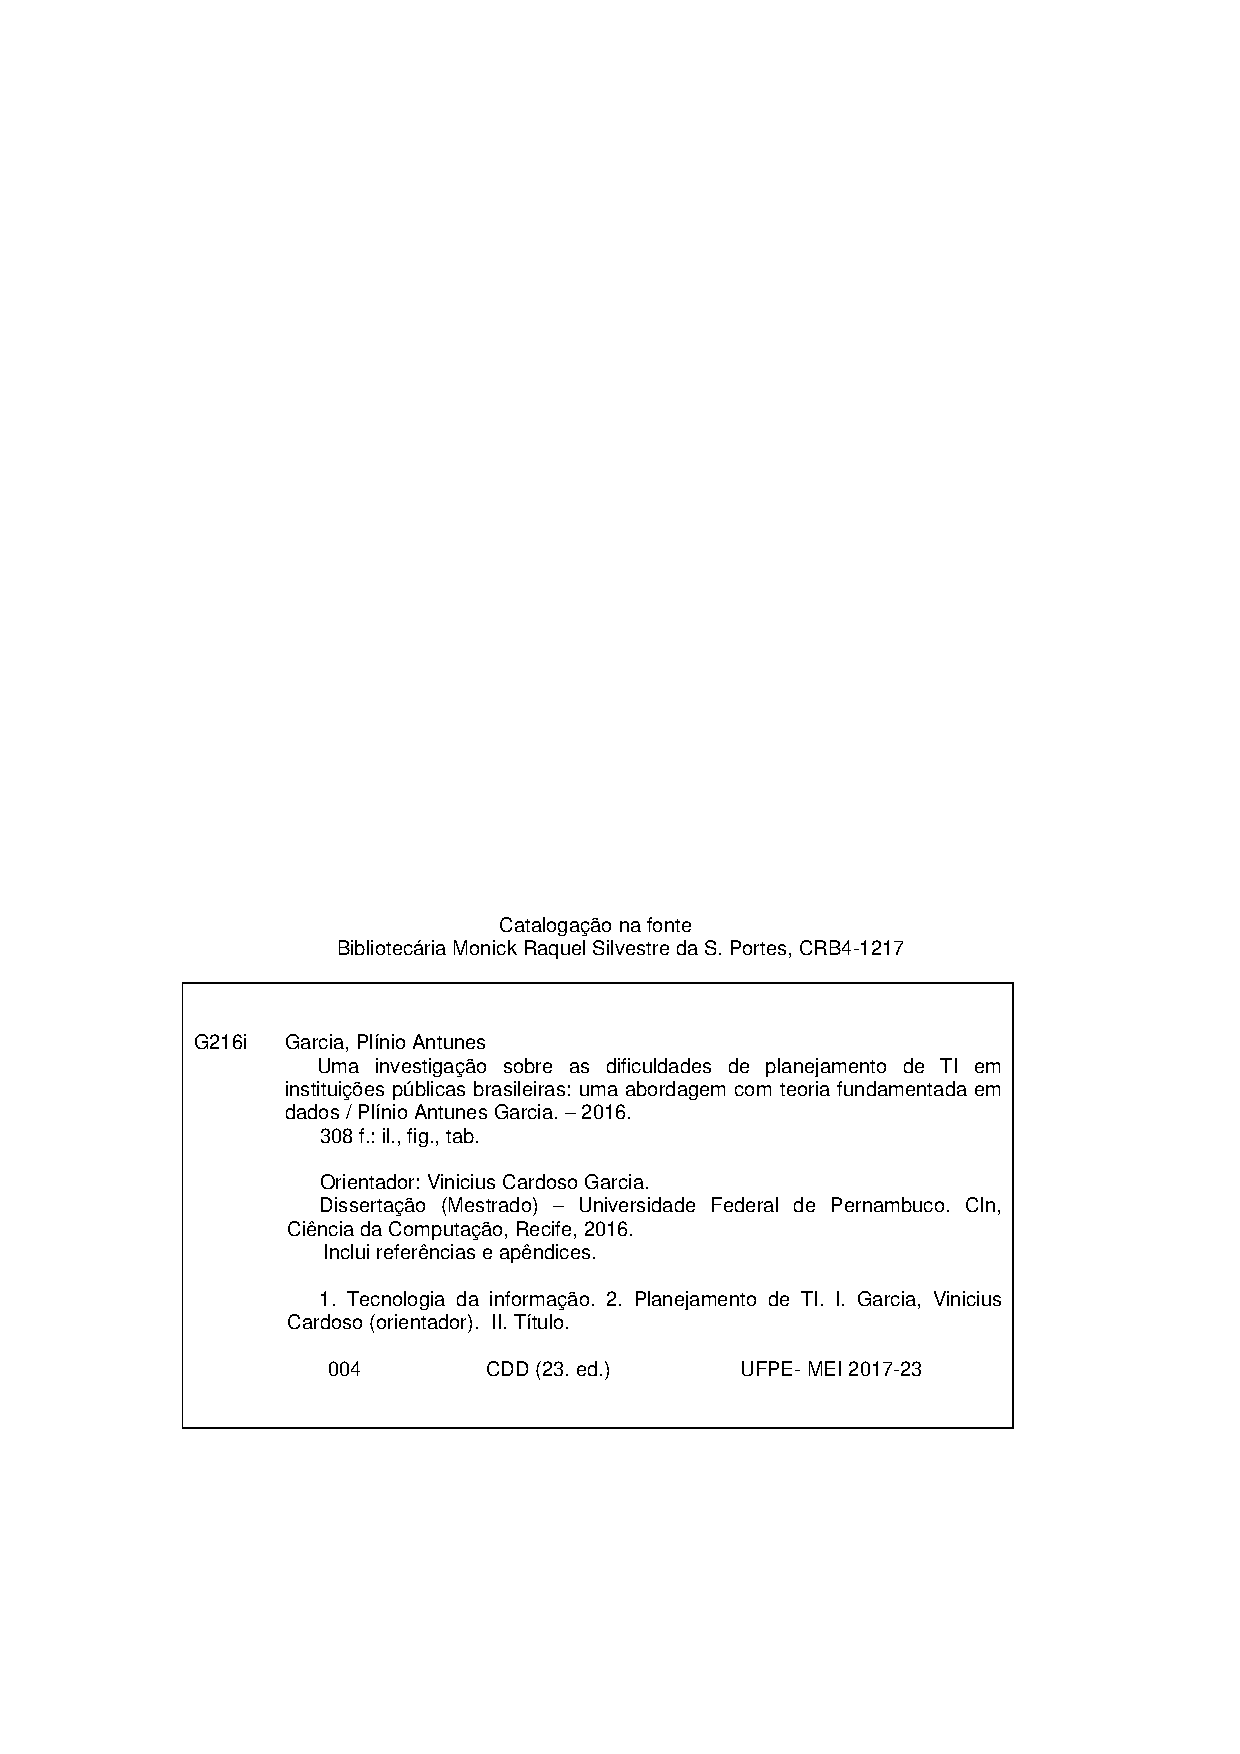
\includepdf[pages=-]{pre-textuais/ficha_catalografica.pdf}
% ---

% ---
% Inserir a ficha bibliografica
% ---

% Isto é um exemplo de Ficha Catalográfica, ou ``Dados internacionais de
% catalogação-na-publicação''. Você pode utilizar este modelo como referência. 
% Porém, provavelmente a biblioteca da sua universidade lhe fornecerá um PDF
% com a ficha catalográfica definitiva após a defesa do trabalho. Quando estiver
% com o documento, salve-o como PDF no diretório do seu projeto e substitua todo
% o conteúdo de implementação deste arquivo pelo comando abaixo:
%
% \begin{fichacatalografica}
%     \includepdf{fig_ficha_catalografica.pdf}
% \end{fichacatalografica}

%\begin{fichacatalografica}
%	\sffamily
%	\vspace*{\fill}					% Posição vertical
%	\begin{center}					% Minipage Centralizado
%	\fbox{\begin{minipage}[c][8cm]{13.5cm}		% Largura
%	\small
%	\imprimirautor
%	%Sobrenome, Nome do autor
%	
%	\hspace{0.5cm} \imprimirtitulo  / \imprimirautor. --
%	\imprimirlocal, \imprimirdata-
%	
%	\hspace{0.5cm} \pageref{LastPage} p. : il. (algumas color.) ; 30 cm.\\
%	
%	\hspace{0.5cm} \imprimirorientadorRotulo~\imprimirorientador\\
%	
%	\hspace{0.5cm}
%	\parbox[t]{\textwidth}{\imprimirtipotrabalho~--~\imprimirinstituicao,
%	\imprimirdata.}\\
%	
%	\hspace{0.5cm}
%		1. Palavra-chave1.
%		2. Palavra-chave2.
%		2. Palavra-chave3.
%		I. Orientador.
%		II. Universidade xxx.
%		III. Faculdade de xxx.
%		IV. Título 			
%	\end{minipage}}
%	\end{center}
%\end{fichacatalografica}
% ---

% ---
% Inserir errata
% ---
%\begin{errata}
%Elemento opcional da \citeonline[4.2.1.2]{NBR14724:2011}. Exemplo:

%\vspace{\onelineskip}

%FERRIGNO, C. R. A. \textbf{Tratamento de neoplasias ósseas apendiculares com
%reimplantação de enxerto ósseo autólogo autoclavado associado ao plasma
%rico em plaquetas}: estudo crítico na cirurgia de preservação de membro em
%cães. 2011. 128 f. Tese (Livre-Docência) - Faculdade de Medicina Veterinária e
%Zootecnia, Universidade de São Paulo, São Paulo, 2011.

%\begin{table}[htb]
%\center
%\footnotesize
%\begin{tabular}{|p{1.4cm}|p{1cm}|p{3cm}|p{3cm}|}
%  \hline
%   \textbf{Folha} & \textbf{Linha}  & \textbf{Onde se lê}  & \textbf{Leia-se}  \\
%    \hline
%    1 & 10 & auto-conclavo & autoconclavo\\
%   \hline
%\end{tabular}
%\end{table}

%\end{errata}
% ---

% ---
% Inserir folha de aprovação
% ---

% Isto é um exemplo de Folha de aprovação, elemento obrigatório da NBR
% 14724/2011 (seção 4.2.1.3). Você pode utilizar este modelo até a aprovação
% do trabalho. Após isso, substitua todo o conteúdo deste arquivo por uma
% imagem da página assinada pela banca com o comando abaixo:
%
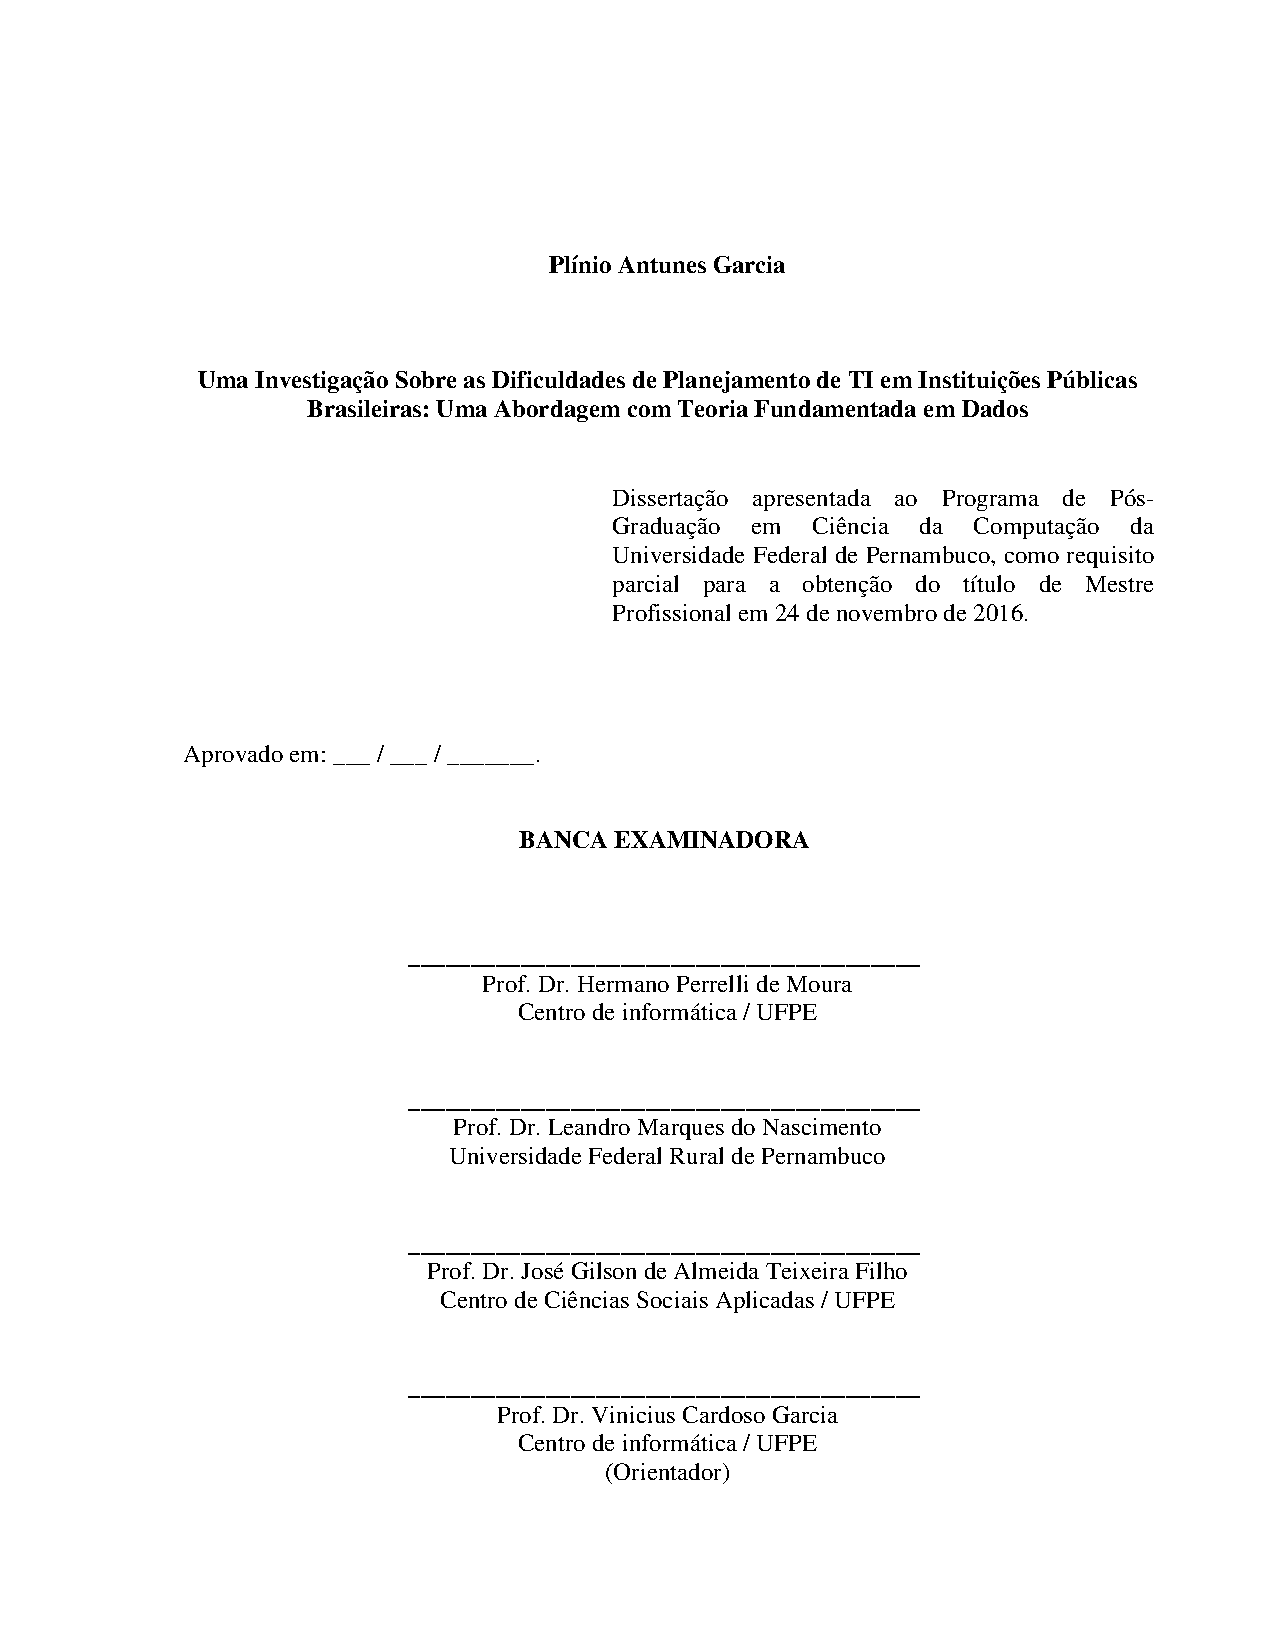
\includepdf[pages=-]{pre-textuais/folha_aprovacao.pdf}
%
%\begin{folhadeaprovacao}

%  \begin{center}
%    {\ABNTEXchapterfont\large\imprimirautor}

%    \vspace*{\fill}\vspace*{\fill}
%    \begin{center}
%      \ABNTEXchapterfont\bfseries\Large\imprimirtitulo
%    \end{center}
%    \vspace*{\fill}
    
%    \hspace{.45\textwidth}
%    \begin{minipage}{.5\textwidth}
%        \imprimirpreambulo
%    \end{minipage}%
%    \vspace*{\fill}
%   \end{center}
        
%   Trabalho aprovado. \imprimirlocal, 24 de novembro de 2012:

%   \assinatura{\textbf{\imprimirorientador} \\ Orientador} 
%   \assinatura{\textbf{Professor} \\ Convidado 1}
%   \assinatura{\textbf{Professor} \\ Convidado 2}
   %\assinatura{\textbf{Professor} \\ Convidado 3}
   %\assinatura{\textbf{Professor} \\ Convidado 4}
      
%   \begin{center}
%    \vspace*{0.5cm}
%    {\large\imprimirlocal}
%    \par
%    {\large\imprimirdata}
%    \vspace*{1cm}
%  \end{center}
  
%\end{folhadeaprovacao}
% ---

% ---
% Dedicatória
% ---

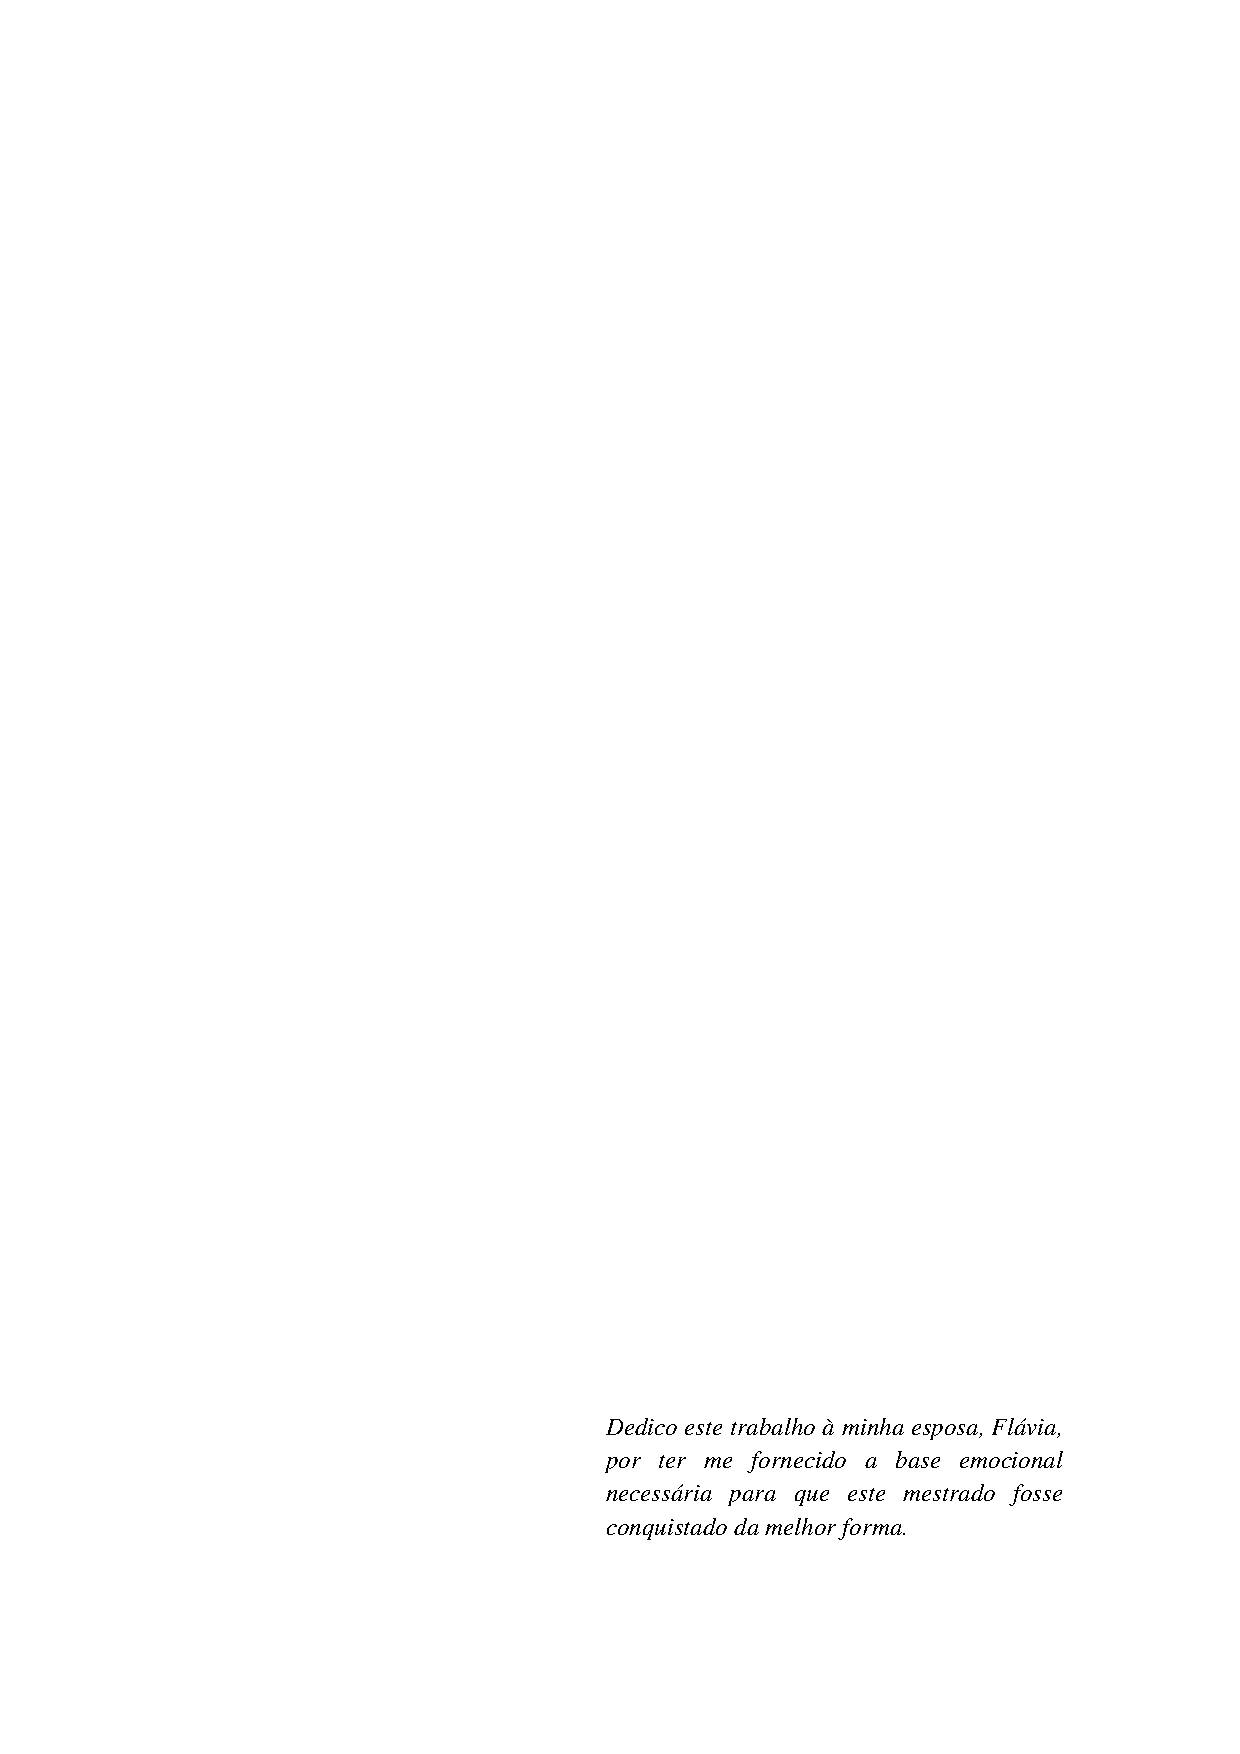
\includepdf[pages=-]{pre-textuais/dedicatoria.pdf}

%\begin{dedicatoria}
%    \vspace*{\fill}
%    \hspace{\stretch{2}}
%   \begin{flushright}
%   \noindent
%   \textit{Dedico este trabalho à minha esposa, Flávia, por ter me fornecido a base emocional necessária para que
%   este mestrado fosse conquistado da melhor forma.}
%   \end{flushright}
%   \vspace*{\fill}
%\end{dedicatoria}
% ---

% ---
% Agradecimentos
% ---
\begin{agradecimentos}
Agradeço à minha família, principalmente aos meus pais, Sônia e Antonio, por ter me ensinado que a educação é um patrimônio
para toda a vida e por ter me dado o suporte necessário para seguir neste caminho.

Ao meu amor, Flávia, por estar sempre ao meu lado, por me ajudar a perseverar nos estudos nos momentos mais difíceis, pelo companheirismo, inspiração e por ser minha maior incentivadora.

Aos meus colegas de trabalho do Instituto Federal Catarinense e a esta instituição que, junto com a UFPE e demais instituições, possibilitou a oportunidade deste mestrado à vários servidores de todo o país.

Aos companheiros de mestrado que permitiram um aprendizado de vida além da sala de aula. E, especialmente, aos amigos do flat CDU por compartilhar as angústias, alegrias e pela grande amizade construída.

Aos professores do Centro de Informática da UFPE pelos seus ensinamentos, especialmente o professor Vinicius Garcia na orientação desta pesquisa, e aos funcionários do CIn que contribuíram para que este curso fosse realizado.

\end{agradecimentos}
% ---

% ---
% Epígrafe
% ---
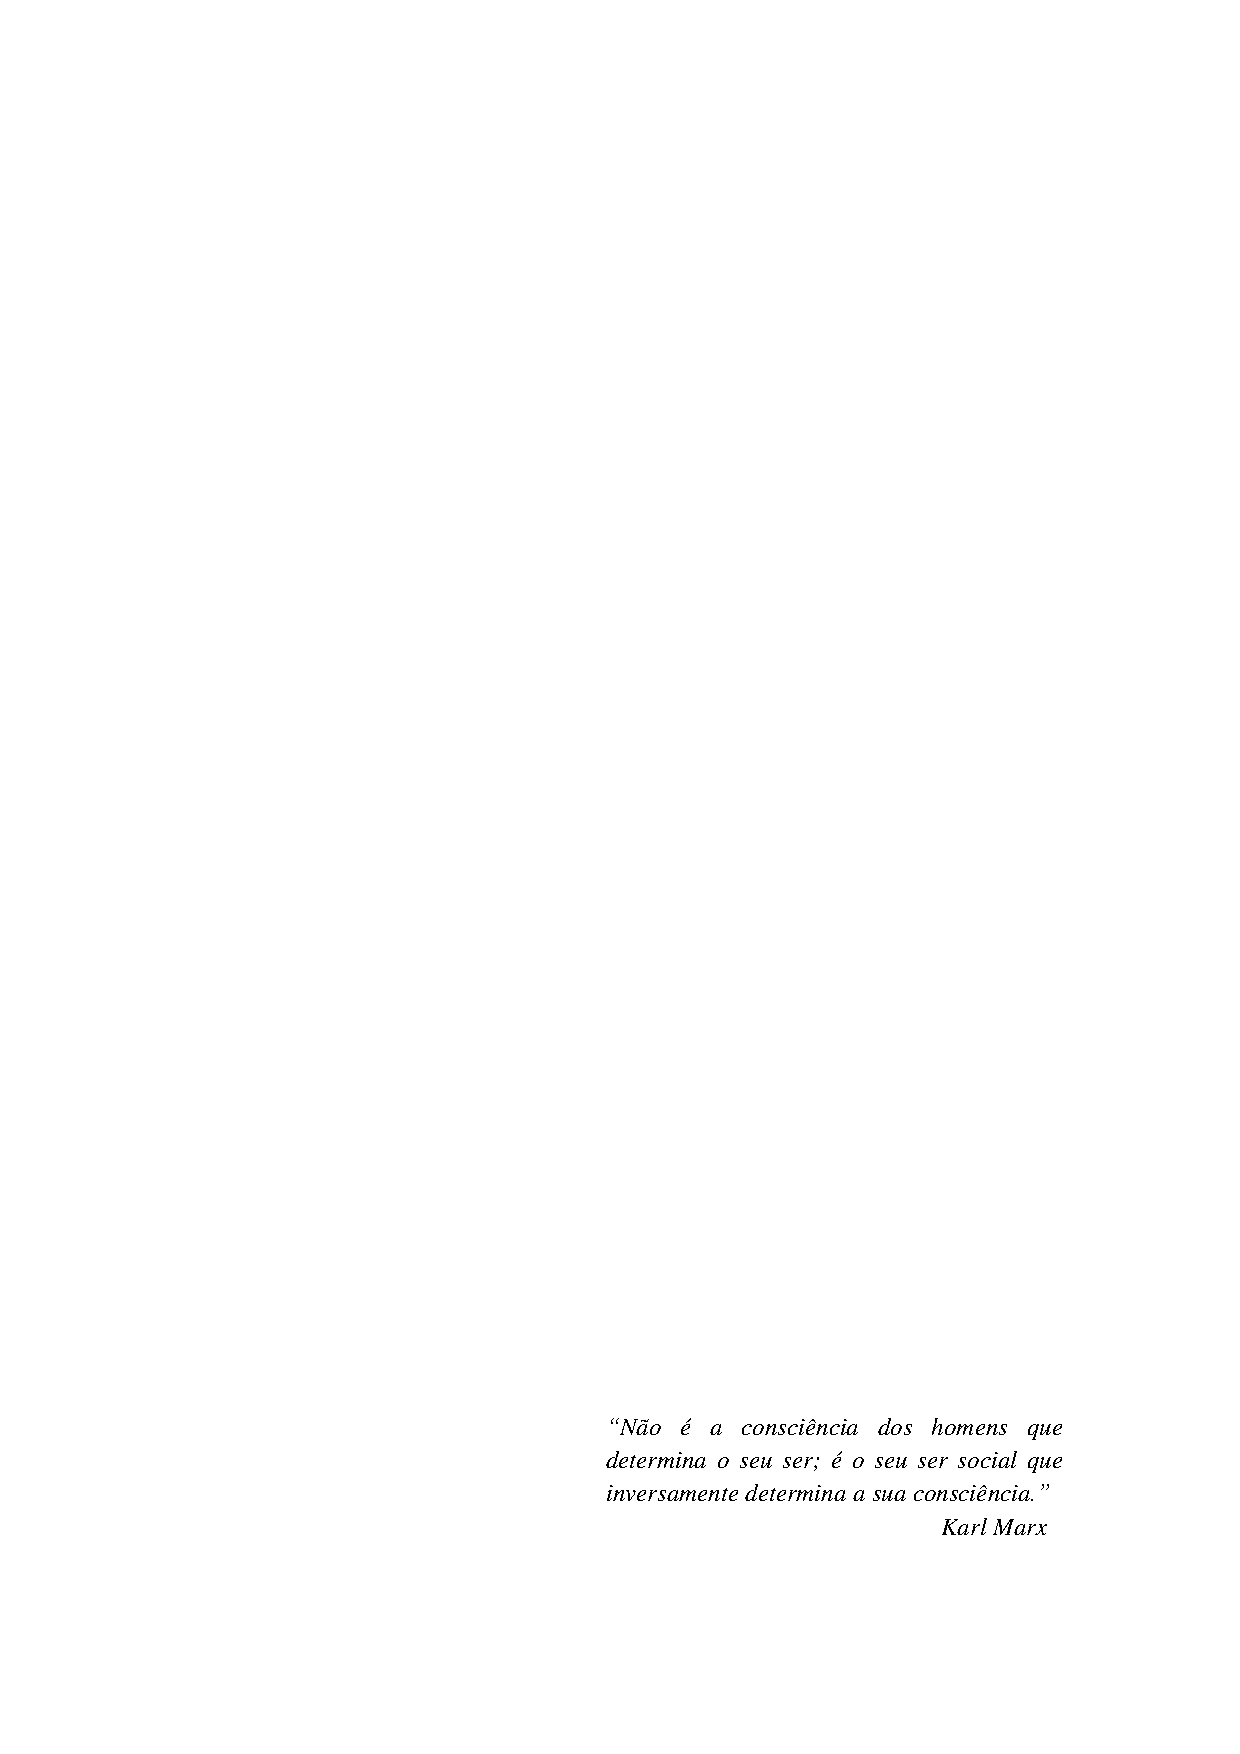
\includepdf[pages=-]{pre-textuais/epigrafe.pdf}

%\begin{epigrafe}
%    \vspace*{\fill}
%    \hspace{\fill}
%	\begin{flushright}
%		\textit{``Não é a consciência dos homens que determina o seu ser; é o seu ser social que inversamente determina a sua consciência."}
%		\\Karl Marx
%	\end{flushright}
%\end{epigrafe}
% ---

% ---
% RESUMOS
% ---

% resumo em português
\setlength{\absparsep}{18pt} % ajusta o espaçamento dos parágrafos do resumo
\begin{resumo}
%Contexto: 
Assim como em organizações privadas, os órgãos públicos devem realizar processos de planejamento para cumprir seus objetivos. O governo brasileiro determina que as instituições federais elaborem um Plano Diretor de TI (PDTI), importante instrumento de planejamento das atividades de TI. O PDTI permite que a instituição tenha controle sobre os recursos gastos com tecnologia da informação, melhore o alinhamento estratégico e minimize os riscos relacionados aos ativos de TI.
%Problema:
Contudo, relatórios do Tribunal de Contas da União (TCU) apresentam índices preocupantes com relação à adoção do PDTI. Apesar de seus conhecidos benefícios e de ser obrigatório nos órgãos da administração pública federal, o PDTI não está sendo adotado por um número considerável de instituições. Além disso, pouco mais da metade dos órgãos que possuem PDTI fazem o vínculo das ações de TI com os objetivos estratégicos da instituição, ou seja, apresentam deficiências de alinhamento estratégico.
%Objetivo:
Esta pesquisa busca compreender de forma abrangente as dificuldades que resultam nos números insatisfatórios apresentados pelo TCU. O objetivo principal desta pesquisa consistiu em elaborar teoria fundamentada em dados que apresente uma relação de causa e consequência entre os elementos que restringem a elaboração do PDTI. Os resultados apresentam duas teorias, a primeira, com as razões da ausência do PDTI em algumas instituições e, a segunda, com as causas das dificuldades encontradas durante a elaboração do PDTI. Utilizando o mesmo método, Grounded Theory, foi possível relacionar os elementos das teorias fundamentadas com um conjunto de 5 processos e 48 melhores práticas de planejamento de TI. Desta forma, este trabalho apresenta uma forma de minimizar os problemas encontrados na elaboração do PDTI.

%A partir do método Grounded Theory, pôde-se sugerir um conjunto de melhores práticas de planejamento estratégico de TI para minimizar as causas do problema levantadas durante a elaboração da teoria.
%Método:
%Através da Grounded Theory, um método de pesquisa qualitativa, foi possível extrair duas teorias fundamentadas nos dados coletados com membros de instituições públicas federais brasileiras. A primeira aborda as razões de instituições que não possuem PDTI e a segunda teoria aborda as causas das principais dificuldades que as instituições enfrentaram para elaborar seus PDTI.
%A primeira aborda as razões de instituições não adotarem o PDTI e a segunda teoria aborda as causas das principais dificuldades que as instituições enfrentaram para elaborarem seus PDTI.


 \textbf{Palavras-chave}: Planejamento de TI. Plano Diretor de TI. PDTI. Instituições Públicas Brasileiras. Melhores Práticas de Planejamento de TI. Grounded Theory.
\end{resumo}

% resumo em inglês
\begin{resumo}[Abstract]
 \begin{otherlanguage*}{english}
As with private organizations, public organs should execute planning processes to achieve their goals. The Brazilian government determines that federal institutions develop an IT Director Plan (PDTI), an important tool for planning of IT activities. The PDTI permits a better control of the resources spent with information technology in the organizations, it also improves the strategic alignment and reduces the risks about IT asset. However, government reports show worrying indicators regarding to the application of PDTI by the public organs. Despite the known benefits and the obligation of using PDTI in the public organs, many haven’t used it. Moreover, almost a half of the group that uses PDTI doesn’t connect the IT actions with the strategic goals of the organ, which means that they have a gap in their strategic alignment. This research seeks to understand the difficulties that result in unsatisfactory indicators related to the PDTI. The main goal of this research was elaborate a theory which shows a cause relation between the elements which Works like a barrier to the use of PDTI. The results present two theories, the first one, the reasons for the absence of PDTI in some institutions, and the second, the causes of difficulties encountered during the elaboration of PDTI. Using the same method, Grounded Theory, it was possible to relate the elements of grounded theories with a set of 5 processes and 48 best practices of IT planning. In this way, this work presents a way to minimize the problems found in the elaboration of the PDTI.

%Starting with the grounded theory, it was possible to suggest a set of the best practise for the IT strategic planning to minimize the causes of the gaps founded. By using Grounded Theory, a qualitative research methodology, it was possible to extract two grounded theories based on data obtained from workers of Brazilian public organs. The first one is related to the reasons that makes the organizations not use the PDTI and the second theory shows the causes of the difficulty founded during the development of the PDTI.


   \vspace{\onelineskip}
 
   \noindent 
   \textbf{Keywords}: IT Strategic Planning. Brazilian Government Agencies. Best Practices. Grounded Theory.
 \end{otherlanguage*}
\end{resumo}
% ---

% ---
% inserir lista de ilustrações
% ---
\pdfbookmark[0]{\listfigurename}{lof}
\listoffigures*
\cleardoublepage
% ---

% ---
% inserir lista de tabelas
% ---
\pdfbookmark[0]{\listtablename}{lot}
\listoftables*
\cleardoublepage
% ---

% ---
% inserir lista de abreviaturas e siglas
% ---
\begin{siglas}
\item AC: Notas de Codificação Axial
\item APF: Administração Pública Federal
\item EGD: Estratégia de Governança Digital
\item EGTI: Estratégia Geral de Tecnologia da Informação
\item GT: Grounded Theory
\item IF: Institutos Federai
\item MA: Notas de Microanálise
\item MMPE: Modelo de Maturidade para Planejamento Estratégico de SI/TI
\item MP: Melhores Práticas
\item OC: Notas de Codificação Aberta
\item PDTI: Plano Diretor de Tecnologia da Informação
\item PEI: Planejamento Estratégico Institucional
\item PETI: Planejamento Estratégico de Tecnologia da Informação
\item SI: Sistemas de Informação
\item SISP: Sistema de Administração dos Recursos de TI
\item SLTI: Secretaria de Logística e Tecnologia da Informação
\item TCU: Tribunal de Contas da União
\item TI: Tecnologia da Informação
\item TIC: Tecnologia da Informação e Comunicação
\item UF: Universidades Federai

\end{siglas}
% ---

% ---
% inserir lista de símbolos
% ---
%\begin{simbolos}
%  \item[$ \Gamma $] Letra grega Gama
%  \item[$ \Lambda $] Lambda
%  \item[$ \zeta $] Letra grega minúscula zeta
%  \item[$ \in $] Pertence
%\end{simbolos}
% ---

% ---
% inserir o sumario
% ---
\pdfbookmark[0]{\contentsname}{toc}
\tableofcontents*
\cleardoublepage
% ---



% ----------------------------------------------------------
% ELEMENTOS TEXTUAIS
% ----------------------------------------------------------
\textual
% É aconselhável criar cada capítulo em um arquivo à parte, digamos
% "capitulo1.tex", "capitulo2.tex", ... "capituloN.tex" e depois
% incluí-los com:
%
\setcounter{page}{15}
\chapter{Introdução}
%apenas contexto, não tem que expor o problema
%Falar sobre a importancia e o papel da gestão/governança de TI no setor público;
A governança de Tecnologia da Informação (TI) é composta de estruturas organizacionais, processos, controles e outros componentes com objetivo de usar a TI para agregar valor ao negócio das organizações, com riscos controlados e aceitáveis. A governança de TI pode evitar ou reduzir deficiências na gestão de uma organização, tais como problemas na gestão de pessoas, em processos de planejamento, projetos e contratações \cite{weill:04,tcu:14}.

No âmbito da Administração Pública Federal\footnote{"A APF corresponde ao conjunto de órgãos da administração direta, autárquica e fundacional. Não fazem parte empresas públicas e
sociedades de economia mista." \cite{egd:16}} (APF) a governança de TI é referenciada com termos variados, como governo digital e governo eletrônico. A governança de TI na APF tem seu início na década de 2000 marcado por um projeto denominado e-Gov, cujo objetivo era priorizar o uso das tecnologias da informação e comunicação (TIC) para democratizar o acesso à informação \cite{egd:16}.

Até a presente data, o governo brasileiro vem amadurecendo seus processos de governança de TI. Destaca-se neste período a criação da Instrução Normativa número 4 (IN 04/2008), que regula as contratações de TI na APF \cite{in04:08}. No ano seguinte, em 2009, entrou em vigor um importante instrumento de governança de TI para a administração pública brasileira, a Estratégia Geral de Tecnologia da Informação (EGTI), com o objetivo de estabelecer as bases estratégicas para a melhoria da gestão de TI nos órgãos \cite{egti:08}.

Em consulta no portal da transparência do governo federal\footnote{A consulta realizada no portal da transparência na funcionalidade "Consultas por Função Orçamentária" na aba "Despesas", selecionando a finalidade "Tecnologia da Informação".} é possível verificar que, apenas no ano de 2015, as despesas com TI somam R\$ 3,445 bilhões. Diante disso, além de utilizar a tecnologia para promover serviços públicos digitais, viabilizar o acesso à informação e ampliar a participação social na construção de políticas públicas, é do interesse do governo federal administrar o orçamento destinado à TI de forma à otimizar os recursos e reduzir os riscos \cite{egd:16}.

Nos órgãos que compõem a APF o planejamento é um princípio fundamental estabelicido no Decreto Lei 200/1967. Desde o início da vigência da EGTI os órgãos do poder executivo federal são obrigados a planejar as ações que envolvem sistemas de informação (SI) e tecnologia da informação através do planejamento de TI \cite{egti:08}. Portanto, todas as organizações públicas, devem desenvolver processos de planejamento e de monitoramento nos níveis institucionais e na área de TI, permitindo assim, melhoria dos serviços de tecnologia prestados ao cidadão e melhor emprego dos orçamentos destinados à TI \cite{tcuManual:07}. 

O principal instrumento de planejamento de TI na APF, denominado Plano Diretor de Tecnologia da Informação (PDTI) é previsto como instrumento obrigatório desde a primeira versão da IN 04/2008 e da EGTI \cite{in04:08, egti:08}. O PDTI possibilita às instituições realizar o diagnóstico, planejamento e gestão dos recursos e processos de TI visando alinhamento com os objetivos estratégicos da instituição.


\section{Motivação e Caracterização do Problema}

Apesar do embasamento legal, a gestão de TI dos órgãos públicos federais não tem atendido satisfatoriamente a necessidade de planejamento. Isto é evidenciado através de uma pesquisa realizada periodicamente pelo Tribunal de Contas da União (TCU), que busca apresentar um Perfil da Governança de TI (Perfil GovTI) dos entes da APF. Os números apresentados nas pesquisas de 2007, 2010, 2012 e 2014 \cite{tcu:14} são apresentados no gráfico da Figura \ref{figura:grafico_tcu}.

\begin{figure}[h]
\centering % para centralizarmos a figura
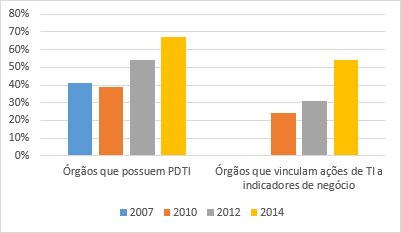
\includegraphics[width=10cm]{figuras/grafico_tcu.png}
\label{figura:grafico_tcu}
\caption{Evolução do PDTI - Perfil GovTI}
\end{figure}

Conforme ilustrado na Figura \ref{figura:grafico_tcu}, os resultados do levantamento de 2014, relatório mais recente até a presente data, apontam que 67\% dos órgãos pesquisados adotam o PDTI, ou seja, 33\% não cumprem as recomendações e determinações acerca da elaboração do PDTI. Ainda em 2014, apenas 54\% das organizações fazem o vínculo das ações de TI a indicadores e metas de negócio. O nível de adoção dessa prática é preocupante, haja vista que a TI deve existir para atender às necessidades do negócio e não dela própria. Desse modo, sem a vinculação das ações de TI aos indicadores e metas de negócio, fica difícil de avaliar a efetividade e a própria necessidade dessas ações \cite{tcu:14}. 

O TCU conclui que apesar da evolução identificada, a situação ainda não pode ser considerada aceitável. Portanto, não é cabível que muitas organizações continuem sem PDTI, considerando a obrigatoriedade estabelecida em normativas e a importância que o planejamento de TI representa para o desempenho da organização. Também é preocupante que, dentre as organizações que possuem PDTI, a qualidade e eficiência do planejamento esteja comprometida uma vez que não possuem o devido compromisso com a estratégia institucional \cite{tcu:14}.

Alguns trabalhos acadêmicos se dedicaram a pesquisar a complexidade do planejamento de TI nas instituições públicas brasileiras com o intuito de contribuir para a melhoria deste cenário \cite{paula:12, barros:13, prando:15}. Por meio de diversos métodos as pesquisas relacionadas a este tema partem de premissas, hipóteses ou modelos pré-estabelecidos acerca das razões que levam aos índices insatisfatórios de planejamento de TI. 

Alguns fatores que influenciam no problema de planejamento de TI nas instituições foram levantados na literatura, no entanto não foram encontrados trabalhos com uma abordagem que permita descobrir as razões que levam aos fatores restritivos do planejamento de TI, ou seja, há pesquisas que apontam para elementos influenciadores no PDTI, porém ainda carece de uma abordagem mais abrangente que elucide a relação entre estes elementos \cite{paula:12, barros:13, prando:15}. 

A presente pesquisa se propõe a preencher esta lacuna identificando tais fatores partindo de fatos descritos por quem está diretamente envolvido no problema e analisando os dados com um método que permite trazer à tona uma relação de causalidade entre os elementos. Em um exemplo hipotético, um dos fatores que restringe a elaboração do planejamento de TI é a ``falta de pessoal capacitado''. A relação de causalidade permite compreender quais outros fatores estão relacionados diretamente a este. Por exemplo, pode-se descobrir que o fator ``restrições orçamentárias'' esteja causando a ``falta de cursos de capacitação'' que, por sua vez, é a causa da ``falta de pessoal capacitado''. As relações entre fatores permitem maior fundamentação ao apontar a causa de um determinado problema.

Diante do exposto, a questão de pesquisa que esta dissertação busca responder é expressada como segue:

\textit{Dados do TCU revelam que muitos entes da Administração Pública Federal não cumprem a determinação de realizar o planejamento da TI. Além disso, nos planos de TI dos órgãos que o fazem, são encontradas deficiências que comprometem sua eficácia. Em suma, a falta de planejamento de TI evidencia o baixo nível de maturidade em governança de TI nestas instituições. A atividade de planejamento envolve aspectos técnicos e sociais, diante disso, pergunta-se: quais os fatores que dificultam o processo de elaboração do planejamento de TI e qual a relação entre tais fatores?}
	
\section{Metodologia}
Esta pesquisa iniciou-se com uma revisão informal da literatura com o intuito de investigar os trabalhos mais recentes relacionados à temática do planejamento de TI no setor público. Também foi utilizada análise documental para levantar estatísticas e conclusões dos órgãos de controle acerca do tema.

O trabalho empírico iniciou-se com a coleta de dados. O método de coleta através de questionário eletrônico foi definido visando atingir o maior número possível de instituições no país. Os dados coletados foram as entradas para a etapa principal da pesquisa, a análise. Após a análise dos dados, também foi utilizado questionário eletrônico para a avaliação dos resultados.

O método indutivo predomina nesta pesquisa, pois parte-se de fatos, de situações presentes na realidade de instituições públicas e que deseja conhecer as causas. A \textit{Grounded Theory} (GT) atua como método indutivo de natureza qualitativa baseada na análise sistemática dos dados \cite{patton:90, corbin:98}. O \autoref{capitulo:metodo_pesquisa} é dedicado ao detalhamento de cada etapa do processo de pesquisa.

\section{Objetivos e Contribuições}

O objetivo geral desta pesquisa é identificar empiricamente\footnote{"Empírico significa guiado pela evidência obtida em pesquisa científica sistemática e controlada" \cite{kerlinger:80}.}, através de uma teoria fundamentada em dados, os fatores, e suas relações, que dificultam ou impedem a elaboração do planejamento de TI em instituições públicas federais brasileiras. Assim, diante da compreensão destes fatores, seria possível propor práticas para a melhoria deste cenário.

Os objetivos específicos que este trabalho visa atingir são:
\begin{enumerate}
\item Elaborar teoria fundamentada em dados sobre os problemas da elaboração do planejamento de TI apresentando causa, fenômeno e consequência;
\item Enfatizar as melhores práticas de planejamento estratégico de TI aplicáveis à teoria obtida.
\end{enumerate}

Além dos objetivos expostos anteriormente, algumas contribuições podem ser destacadas como a própria utilização do método \textit{Grounded Theory} no contexto do planejamento de TI em setores públicos. Todo o processo de análise dos dados foi metodicamente documentado e poderá contribuir com futuras pesquisas que busquem criar teorias fundamentadas em dados.

Apesar de uma revisão sistemática não fazer parte do escopo deste trabalho, esta pesquisa contribui com a revisão da literatura apresentando os trabalhos mais recentes relacionados ao tema de planejamento de TI no setor público brasileiro. Foram destacados nestas pesquisas os fatores que, de acordo com cada autor, são condicionantes para o sucesso de um planejamento de TI em instituições públicas.

Por fim, esta pesquisa se propõe a contribuir para elucidar o problema da elaboração do planejamento de TI nos órgãos federais e, com isto, fornecer os insumos para que as instituições possam melhorar seus PDTI. Esta contribuição, a longo prazo, pode resultar no melhor emprego do orçamento público com a tecnologia da informação e também para melhoria na prestação dos serviços.


\section{Escopo}
Com relação as áreas do conhecimento, esta pesquisa está inserida no campo da ciência da computação, especificamente no contexto da governança de tecnologia da informação. A área da administração contribuiu com alguns fundamentos teóricos acerca do tópico planejamento estratégico. O método utilizado, oriundo das ciências sociais, também é uma área que esta pesquisa toca.

Em relação à abrangência e aplicação da pesquisa, este trabalho está limitado às instituições da Administração Pública Federal. Tomou-se como amostragem, as instituições federais de ensino técnico e superior. Esta decisão se deve ao fato do pesquisador trabalhar em uma instituição deste nicho, o que trouxe alguma empatia com relação ao tema e também facilitou o contato com membros de outras instituições para a coleta de dados.

A abordagem desta pesquisa consiste em utilizar um método científico, \textit{Grounded Theory}, para compreender o problema de pesquisa e elaborar uma teoria com fundamentação na realidade, ou seja, teorias que expliquem o problema de planejamento de TI exposto neste capítulo. De posse das teorias fundamentadas nos dados, os fatores causadores das dificuldades na elaboração do planejamento de TI são expostos e pode-se, enfim, propor um mapeamento das melhores práticas de planejamento estratégico de SI/TI que podem minimizar as causas do problema.

É importante destacar que não está dentro do escopo deste trabalho:

\begin{itemize}
\item Elaboração de uma teoria para os problemas de planejamento de TI de organizações privadas;
\item Elaboração de um plano operacional para a solução dos problemas de planejamento de TI.
\end{itemize}

Por fim, destaca-se que o objeto de pesquisa consiste nos fatores relacionados ao processo de elaboração do planejamento de TI. Portanto, não faz parte do escopo desta pesquisa as questões acerca da aplicação ou execução do planejamento de TI.
	
\section{Organização da Dissertação}
Esta dissertação está organizada em sete capítulos. A introdução apresentou o contexto da pesquisa, motivação e caracterização do problema a ser pesquisado. Além disso, este primeiro capítulo abordou o método a ser utilizado, os objetivos, contribuições e a definição do escopo da pesquisa.

O segundo capítulo, Método de Pesquisa, detalha cada etapa do processo da pesquisa incluindo a apresentação dos princípios básicos do método \textit{Grounded Theory} e como este método se enquadra no contexto desta pesquisa.

O terceiro capítulo, Referencial Teórico, tem o objetivo de abastecer o leitor com os principais conceitos relacionados ao tema desta pesquisa. Neste capítulo são abordados: o alinhamento estratégico, o planejamento de TI e o planejamento de TI no setor público, incluindo leis, normativas e modelos.

%O quarto capítulo apresenta os trabalhos relacionados ao objetivo desta pesquisa, ou seja, trabalhos que abordam os problemas que norteiam o planejamento de TI nas instituições púbicas federais.

O quarto capítulo constitui a parte principal do desenvolvimento desta pesquisa, a Análise dos Problemas de Planejamento de TI em Instituições Públicas Brasileiras. Este capítulo descreve a pesquisa desde a coleta dos dados, a análise com o método GT, os resultados com as teorias resultantes das análises, além da avaliação dos resultados.

O quinto capítulo, Melhores Práticas de Planejamento de TI Relacionadas ao Problema do PDTI, apresenta uma seleção das melhores práticas de planejamento estratégico de SI/TI que são aderentes aos elementos que compõem o resultado desta pesquisa, ou seja, a teoria fundamenta nos dados.

Por último, o sexto capítulo conclui esta dissertação apresentando as considerações finais, trabalhos relacionados, limitações, contribuições e as perspectivas de trabalhos futuros.
\chapter{Método de Pesquisa}
\label{capitulo:metodo_pesquisa}
O propósito deste capítulo consiste em apresentar o método de pesquisa utilizado na construção deste trabalho. De forma geral, o processo de pesquisa deste trabalho envolveu a coleta de dados, análise e avaliação dos resultados. A coleta de dados se deu através de questionário com questões dissertativas (qualitativas) e optativas (quantitativas) acerca do tema ``Elaboração do PDTI''. A aplicação da \textit{Grounded Theory} (GT), método utilizado para análise dos dados, consistiu na etapa principal da pesquisa se apresentando como instrumento essencial na obtenção dos resultados. Para avaliar os resultados, utilizou-se novamente de um questionário aplicado aos mesmos participantes da etapa de coleta de dados. Desta forma, foi possível avaliar não somente os resultados, mas também a eficácia da GT no contexto deste trabalho. Nas seções seguintes, são apresentados detalhes de cada uma das etapas desta pesquisa sob o ponto de vista metodológico.

\section{Etapas da Pesquisa}
Este trabalho foi segmentado em cinco etapas principais: definições iniciais, coleta de dados, análise, seleção das melhores práticas de planejamento e avaliação dos resultados. Na Figura \ref{figura:processoPesquisa} são apresentadas todas as atividades envolvidas no processo da pesquisa.

\begin{figure}[h]
\centering % para centralizarmos a figura
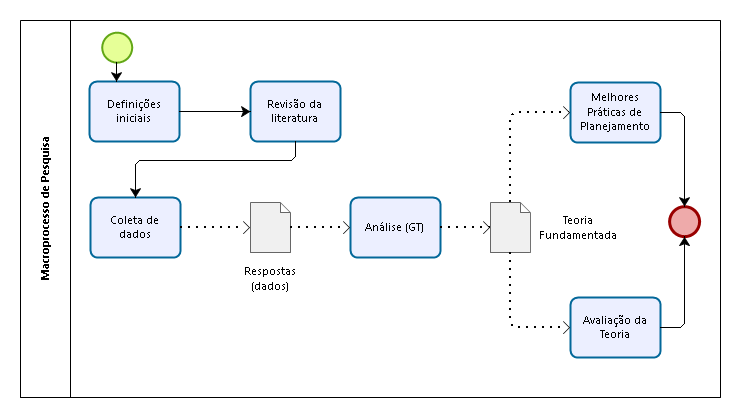
\includegraphics[width=15cm]{figuras/processoPesquisa.png}
\caption{Processo de Pesquisa}
\label{figura:processoPesquisa}
\end{figure}

Na etapa de definições iniciais, a primeira atividade consistiu na percepção e caracterização do problema de pesquisa como segue:
``Dados do TCU revelam que muitos entes da Administração Pública Federal não cumprem a determinação de realizar o planejamento da TI. Além disso, nos planos de TI dos órgãos que o fazem, são encontradas deficiências que comprometem sua eficácia. Em suma, a falta de planejamento de TI evidencia o baixo nível de maturidade em governança de TI nestas instituições.''.

Os dados do relatório do TCU que detalham o cenário que levou à formatação deste problema de pesquisa podem ser encontrados em \citeonline{tcu:14}. Apesar do relatório não revelar a identidade de cada organização, foram avaliadas entidades do poder Executivo, Judiciário, Legislativo e Ministério Público.

A partir do problema de pesquisa pôde-se definir a questão de pesquisa, como segue: ``apesar da obrigatoriedade e dos conhecidos benefícios, o planejamento de TI não é realizado satisfatoriamente nos órgãos públicos brasileiros. A atividade de planejamento envolve aspectos técnicos e sociais, diante disso, pergunta-se: quais os fatores que dificultam o processo de elaboração do planejamento de TI e qual a relação entre tais fatores?''.

Dado o problema de pesquisa, se fez necessário buscar na literatura trabalhos relacionados ao tema. Na revisão da literatura foram utilizadas as bases do Portal de Periódicos da CAPES para pesquisar trabalhos tanto na língua portuguesa quanto na língua inglesa. Os trabalhos retornados pelas \textit{strings} de busca foram filtrados através de eliminação por títulos, resumos, e por fim, eliminação após leitura completa. No capítulo final deste trabalho são apresentados os trabalhos relacionados selecionados na revisão da literatura.

Após a leitura dos trabalhos mais recentes relacionados à temática do planejamento de TI no setor público, foi possível definir o escopo do trabalho e os métodos de pesquisa. Optou-se por uma abordagem qualitativa na qual o método \textit{Grounded Theory} foi  definido como ferramenta de análise dos dados.

%@to-do: colocar uma versão do questionário nos apêndices e dar um jeito de referenciar aqui neste parágrafo.
%@to-do: vou ter que colocar as respostas das perguntas também. Mas acho que talvez seja melhor em um apêndice distinto.
Na etapa seguinte, a coleta de dados ocorreu através de um questionário disponibilizado \textit{on-line} para o público alvo: participantes da elaboração e/ou revisão de PDTI de universidades federais (UFs) e institutos federais de educação, ciência e tecnologia (IFs). Obteve-se 53 respostas de 37 instituições diferentes, sendo 20 UFs, das 63 existentes no país e 17 IFs, dos 41 existentes. Portanto, a pesquisa tem uma amostra de 35,57\% das instituições federais de ensino superior e técnico. O questionário é composto de perguntas dissertativas (qualitativas) e perguntas objetivas (quantitativas), como pode ser visto no \autoref{apendice:a_quest_coleta}.

As respostas coletadas servem como \textit{input} para a etapa de análise dos dados, cujas atividades são as fases de codificação da GT: codificação aberta, codificação axial e codificação seletiva. O resultado da etapa de análise constitui a teoria fundamentada em dados que serve de entrada para a etapa final de avaliação dos resultados.

%@to-do: verificar se quando eu falo do Likert eu devo colocar alguma nota de rodapé ou referenciar alguma obra dele
%@to-do: incluir questionário de avaliação nos apêndices
A etapa de avaliação dos resultados ocorreu por meio de questionário eletrônico com itens de \textit{Likert}, que pode ser visualizado no \autoref{apendice:b_quest_avaliacao}. Os resultados desta etapa e das etapas anteriores são pormenorizadas no Capítulo 4 deste trabalho.

A teoria resultante da análise com \textit{Grounded Theory} também serve de entrada para a etapa de seleção das melhores práticas de planejamento de TI. Nesta etapa, detalhada no Capítulo 5, executou-se novamente técnicas da \textit{Grounded Theory} com o objetivo de relacionar as melhores práticas de planejamento estratégico de TI com os elementos da teoria descoberta na análise dos dados.


\section{Princípios da Grounded Theory}
\label{secao:principios_da_gt}
O termo ``pesquisa qualitativa'' pode ser atribuído às pesquisas cujas descobertas são oriundas de métodos não estatísticos \cite{corbin:98}. De acordo com \citeonline{stern:80}, métodos qualitativos podem ser usados para explorar, de forma substancial, áreas pouco conhecidas ou para se obter um novo entendimento de uma área já conhecida. Pesquisas qualitativas podem se referir, por exemplo, a comportamentos, experiências vividas, emoções, funcionamento organizacional, movimentos sociais e fenômenos culturais \cite{corbin:98}.

A abordagem qualitativa pode ser aplicada através de diversos métodos, como a etnografia, pesquisa-ação e estudos de caso \cite{patton:90}. A definição do método a ser utilizado pode envolver diversas variáveis, como o objetivo de pesquisa, habilidades do pesquisador, participantes e os recursos a serem utilizados na pesquisa \cite{easterbrook:08}.

A proposta apresentada neste trabalho consiste na utilização do método de pesquisa qualitativa \textit{Grounded Theory}  \cite{glaser:68}, ou Teoria Fundamentada em Dados, visando elucidar o problema da elaboração de PDTI nos órgãos públicos brasileiros. Este método foi originalmente desenvolvido pelos sociólogos Barney Glaser e Anselm Strauss no fim da década de sessenta. Com o passar do tempo, os autores da GT desenvolveram pensamentos divergentes sobre aplicação do método, culminando em duas linhas de pensamento: a \textit{Grounded Theory} Glaseriana, descrita por \citeonline{glaser:92}, e a \textit{Grounded Theory} Straussiana, de \citeonline{strauss:87} consolidada com a contribuição de Juliet Corbin \cite{corbin:98}.

\citeonline{niekerk:09} pesquisaram as principais diferenças entre as duas linhas de pensamento da GT. A linha de pensamento Straussiana, vertente a ser adotada na presente pesquisa, parte do princípio que o pesquisador já possui uma questão de pesquisa a ser respondida. Ao contrário, a vertente Glaseriana diz que o pesquisador deve possuir apenas a área do problema em mente, e que a questão de pesquisa emergirá durante a própria pesquisa. Com relação à sensibilidade teórica, a linha Glaseriana conta com a habilidade do pesquisador em gerar seus próprios conceitos e propriedades a partir dos dados. Já a linha Straussiana conta com a sensibilidade do pesquisador ao atribuir significado aos conceitos presentes nos dados.

Apesar das duas vertentes, a GT pode ser definida como um método científico que utiliza um conjunto de procedimentos sistemáticos de coleta e análise dos dados para gerar, elaborar e validar teorias substantivas sobre fenômenos essencialmente sociais, ou processos sociais abrangentes \cite{bandeira:03}. Neste contexto, o termo ``teoria'' pode ser entendido como ``um conjunto de categorias bem desenvolvidas (conceitos) que estão sistematicamente inter-relacionadas através de sentenças de relacionamento (proposições) para formar o esquema teórico que explica um fenômeno social'' \cite[p. 22]{corbin:98}.

Segundo \citeonline{conte:09}, ``a essência do método \textit{Grounded Theory} é que a teoria substantiva emerge dos dados, ou seja, é uma teoria fundamentada em uma análise sistemática dos dados''. Desta forma, o resultado de uma pesquisa que utiliza GT como método traz uma teoria fiel à realidade dos dados, reduzindo a influência dos preconceitos do pesquisador \cite{bandeira:03}. Embora o objetivo da GT seja a descoberta de teorias substantivas, o pesquisador pode optar por apenas algumas das etapas ou procedimentos da GT para satisfazer seus objetivos de pesquisa \cite{corbin:98}.

De acordo com a vertente Straussiana, a GT se baseia na ideia de codificação (\textit{coding}), que é o processo de analisar os dados para identificar conceitos (ou códigos) e categorias \cite{conte:09}. Um conceito (ou código) atribui um nome a um fenômeno de interesse para o pesquisador, ou seja, abstrai um evento, objeto, ação, ou interação que tem algum significado para o pesquisador no contexto de sua pesquisa \cite{corbin:98}. As categorias são conjuntos de conceitos relacionados \cite{birks:11}. O processo de codificação pode ser dividido em três fases: codificação aberta, axial e seletiva.
 
\begin{itemize}  
\item Codificação Aberta: etapa em que o pesquisador varre o material coletado e busca extrair conceitos, categorias e suas propriedades e dimensões;
\item Codificação Axial: nesta etapa ocorre o processo de relacionar categorias entre si e entre as propriedades e dimensões. Através destes relacionamentos é possível traçar proposições acerca do fenômeno estudado;
\item Codificação Seletiva: etapa em que o pesquisador identifica a categoria central do fenômeno e realiza o refinamento da teoria que emerge dos dados.
\end{itemize}

Apesar de serem apresentadas de forma linear, as fases do processo de codificação se sobrepõem e o fluxo admite a circularidade e, por isso, devem ser melhor compreendidas como tarefas do pesquisador e não como etapas de um processo linear \cite{bandeira:03}. Na Figura \ref{figura:GTprocesso} o processo de codificação é apresentado em sua forma iterativa.

\begin{figure}[h!]
\centering % para centralizarmos a figura
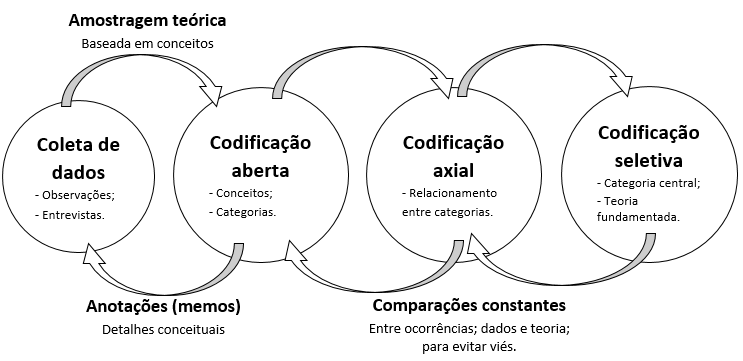
\includegraphics[width=15.5cm]{figuras/GTprocesso.png}
\caption{Processo de análise com \textit{Grounded Theory}, adaptado de \citeonline{cho:14}}
\label{figura:GTprocesso}
\end{figure}

%parágrafo da codificação aberta
A codificação aberta, ou codificação inicial, consiste no mapeamento de conceitos explorando minuciosamente os dados ao ler o material coletado de forma intensiva \cite{conte:09}. Os incidentes ou eventos são agrupados em códigos (conceitos) através da comparação incidente-incidente no intuito de gerar amostragens teóricas e ter evidências suficientes para formar categorias fundamentadas nos dados \cite{bandeira:03}. De acordo com \citeonline{cresswell:98}, durante a codificação aberta pergunta-se: o que o dado está sugerindo? Sob qual ponto de vista? Em qual categoria este dado específico se enquadra?

A codificação axial tem o objetivo de ordenar, sintetizar e organizar os códigos mapeados na codificação aberta e, principalmente, descobrir relações entre eles \cite{cresswell:98}. Neste processo pergunta-se aos dados: ``quando? Onde? Por quê? Quem? Como? Quais as consequências?'' \cite[p. 125]{corbin:98}. Nesta fase o pesquisador relaciona as categorias umas com as outras e com subcategorias, especificando suas propriedades e dimensões fundamentando os relacionamentos nos dados \cite{charmaz:14}. Na Tabela \ref{tabela:conectores} são apresentados os conectores utilizados para caracterizar relacionamentos entre códigos.

\begin{table}[h!]
\centering
\resizebox{\textwidth}{!}{%
\begin{tabular}{|l|l|}
\hline
\rowcolor[HTML]{9B9B9B} 
\textbf{Rótulo} & \textbf{Descrição do relacionamento} \\ \hline
is a & \begin{tabular}[c]{@{}l@{}}O código-origem é um tipo, ou forma, do código-destino encontrada nos \\ dados, e possui um padrão determinado de variação dimensional ao longo\\ das propriedades da categoria (código destino)\end{tabular} \\ \hline
is cause of & O código-origem (condição causal) causa a ocorrência do código-destino \\ \hline
is part of & \begin{tabular}[c]{@{}l@{}}O código-origem é uma parte, que compõe juntamente com outras partes o \\ código destino\end{tabular} \\ \hline
is associated with & \begin{tabular}[c]{@{}l@{}}Os códigos possuem uma ligação entre si que não pôde ser classificada \\ como algum dos relacionamentos anteriores\end{tabular} \\ \hline

\end{tabular}%
}
\caption{Conectores de códigos, adaptado de \citeonline{bandeira:03}}
\label{tabela:conectores}
\end{table}

A terceira e última fase de codificação, chamada de codificação seletiva, tem o objetivo de integrar e refinar as categorias para que, desta forma, seja possível identificar a categoria central do fenômeno pesquisado \cite{corbin:98}. Nesta fase grande parte dos dados foram codificados, as relações entre categorias identificadas e o pesquisador tem condições de inferir a categoria que consegue integrar as demais \cite{bandeira:03}. Notas e diagramas feitos durante as análises podem auxiliar o pesquisador na descoberta da teoria central.



\section{Grounded Theory no Contexto da Pesquisa}
%pq foi escolhida para meu problema
Abordagens quantitativas são muito úteis no sentido de prover indicadores. Porém, restringir a identificação das causas que levaram a obtenção destes indicadores à análise quantitativa pode omitir aspectos relevantes do comportamento dos indivíduos cuja influência não pode ser desprezada \cite{conte:09}. Desta forma, métodos qualitativos são indicados quando busca-se compreender, de forma mais abrangente, todo o fenômeno em estudo ao invés de simplesmente simplificar e produzir similaridades \cite{seaman:99}. Uma vantagem em utilizar métodos qualitativos de pesquisa é a necessidade de o pesquisador se aprofundar na complexidade do problema, ao invés de abstraí-la. Isto resulta em dados mais ricos e mais informativos \cite{seaman:08}.

O problema de pesquisa é o ponto de partida que origina questões de pesquisa abertas, gerais e não formalizadas a priori na forma de hipóteses específicas e fechadas \cite{bandeira:03}. Considerando que (i) a questão de pesquisa deste trabalho não forma uma hipótese específica, ou seja, trata-se de uma questão aberta; (ii) considerando que existem trabalhos com abordagens quantitativas acerca do problema desta pesquisa e que, portanto, podem omitir aspectos relevantes do comportamento humano; (iii) considerando que o objetivo principal desta pesquisa busca compreender um fenômeno de forma abrangente; tem-se um cenário apto para a abordagem qualitativa aplicando o método \textit{Grounded Theory} para responder a questão de pesquisa. 

Portanto, nesta pesquisa a \textit{Grounded Theory} atua como ferramenta fundamental na proposta de identificar e compreender os fatores que dificultam o planejamento de TI em instituições públicas federais. O principal aspecto da abordagem desta pesquisa consiste na formulação de uma teoria fundamentada em dados para o problema do planejamento de TI, ou seja, ao aplicar a GT, os resultados são fiéis à realidade refletida nos dados coletados com os envolvidos na temática estudada, ao contrário de outros métodos que dependem da interpretação do pesquisador. 

De posse dos resultados da aplicação da GT espera-se, como consequência desta pesquisa, propor um conjunto de melhores práticas de planejamento que atinjam as causas encontradas neste trabalho. Tais causas são os elementos da teoria que emerge dos dados que possuem relação de causa com o problema pesquisado, por exemplo, se uma das causas do problema é ``falta de capacitação", então espera-se encontrar um conjunto de melhores práticas cujos resultados minimizem o este elemento causal. Desta forma, é pretendido oferecer um meio de, eventualmente, melhorar os índices de planejamento de TI nas instituições pesquisadas. 

\section{Considerações}
Este capítulo apresentou uma visão geral do processo de pesquisa definido para este trabalho, desde as definições iniciais, coleta de dados, análise com GT, até as atividades de avaliação dos resultados. Dois pontos relevantes, sob a perspectiva metodológica, são: a abordagem qualitativa em um cenário que, tradicionalmente, é avaliado de forma quantitativa; a utilização de 
\textit{Grounded Theory} como método para apoiar na compreensão do fenômeno estudado. 

Há de se destacar que esta pesquisa tem um caráter multidisciplinar, pois abrange não somente a área de tecnologia da informação, mas também aspectos da administração e sociologia, uma vez que visa compreender o comportamento dos indivíduos envolvidos em atividades de gestão em um ambiente regido pela TI. Neste cenário a \textit{Grounded Theory} se torna determinante para compreender os fatores sociotécnicos envolvidos no planejamento de TI. No capítulo seguinte, é apresentado o referencial teórico com os principais conceitos inerentes à temática da pesquisa.
\chapter{Referencial Teórico}
Este capítulo tem como objetivo fornecer os principais conceitos relacionados aos temas: alinhamento estratégico e planejamento de TI. Também é abordado o planejamento de TI no contexto do setor público e seus instrumentos normativos. Por fim, são apresentados detalhes do instrumento de planejamento alvo desta pesquisa, o Plano Diretor de Tecnologia da Informação.

\section{Alinhamento Estratégico}

% sobre estratégia de TI
As organizações necessitam cada vez mais dos Sistemas de Informação (SI) e TI para apoiar a tomada de decisões \cite{rezende:08}. \citeonline{boynton:90} definem estratégia de TI como o conjunto de atividades voltadas para (i) reconhecer oportunidades organizacionais para a utilização de tecnologia da informação; (ii) determinar as necessidades de recursos para explorar as oportunidades; (iii) o desenvolvimento de planos de ação para a execução das oportunidades e para atender as necessidades de recursos. Para \citeonline{earl:89}, estratégia de TI é o plano direcional que decide o que fazer com a TI de uma organização a longo prazo. 

% conceito de alinhamento estratégico de pelo menos dois autores fodas 
A estratégia de TI não lida somente com tecnologia. A estratégia de TI envolve criar ambientes integrados que aumentam a efetividade dos recursos humanos, processos de negócio, estruturas organizacionais e tecnologias de modo a transformar a posição competitiva do negócio \cite{luftmanetal:04}. Alinhamento estratégico, ou alinhamento estratégico de TI, diz respeito à forma com que a estratégia de TI está alinhada ao negócio e como o negócio pode ou deveria estar alinhado com a TI \cite{luftman:04}. 

\begin{figure}[h!]
\centering % para centralizarmos a figura
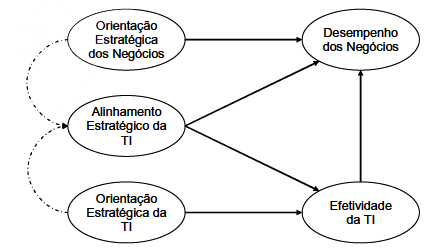
\includegraphics[width=10cm]{figuras/modeloChan.png}
\caption{Modelo de alinhamento estratégico de \citeonline{chan:97}}
\label{figura:modeloChan}
\end{figure}


No modelo de alinhamento estratégico de \citeonline{chan:97}, representado na Figura \ref{figura:modeloChan}, fica explícito que o alinhamento estratégico de TI é composto pela estratégia do negócio e pela estratégia de TI. Além disso, este autor destaca que o alinhamento estratégico é o melhor indicador da efetividade da TI e também do desempenho organizacional.

A estratégia global da organização, dita estratégia do negócio, e as estratégias de TI devem estar alinhadas, ou seja, deve haver harmonia entre as metas e planos de implementação de TI com as metas e a estrutura da organização \cite{luftmanetal:04}. \citeonline{henderson:99} criaram um modelo, representado na Figura \ref{figura:modeloHenderson}, no qual o alinhamento estratégico é apresentado como a adequação e integração funcional entre ambiente externo (mercado) e interno (estrutura organizacional, recursos financeiros, tecnológicos e humanos) para desenvolver as competências e maximizar o desempenho da organização. 

\begin{figure}[h!]
\centering % para centralizarmos a figura
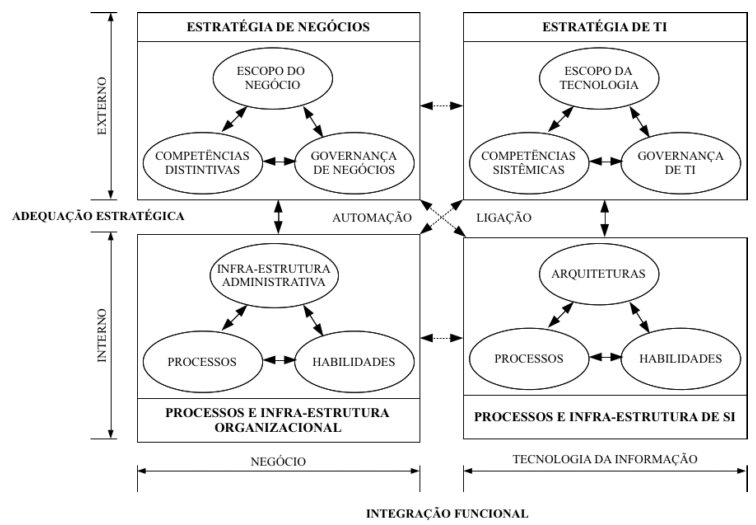
\includegraphics[width=14cm]{figuras/modeloHenderson.png}
\caption{Modelo de alinhamento estratégico de \citeonline{henderson:99}}
\label{figura:modeloHenderson}
\end{figure}

\citeonline{king:88} e \citeonline{chan:97} abordam o alinhamento estratégico sob o ponto de vista dos documentos de planejamento da organização e da área de TI: plano estratégico de negócio (PEN) e o plano estratégico de TI (PETI). Desta forma, o alinhamento estratégico trata-se do alinhamento entre o PEN e o PETI, ou seja, os objetivos presentes no PETI devem estar direcionados ao atendimento dos objetivos organizacionais presentes no PEN.

As empresas que conseguem alinhar suas estratégias de negócio com as estratégias de TI atingem aumento de desempenho em seus negócios \cite{chan:06}. A importância estratégica da TI na gestão de organizações é destacada no \textit{ranking} de preocupações de gestores, no qual o alinhamento estratégico de TI se encontra como preocupação número um nas publicações de 2013, 2014 e, recentemente, em pesquisa de 2015, ficando à frente de temas como segurança/privacidade, produtividade e inovação  \cite{kappelman:15}. Pesquisas tanto da área de TI quanto da área de administração evidenciam o impacto positivo do alinhamento das estratégias de TI com o negócio \cite{reich:96,luftman:96,sabherwal:01};

\citeonline{cragg2002alignment} realizou um estudo com 250 pequenas empresas do Reino Unido e constatou que as empresas que possuem alto índice de alinhamento entre a área de TI e os objetivos da empresa, obtiveram melhor desempenho organizacional do que as empresas com baixo alinhamento estratégico. Neste estudo, por se tratar de pequenas empresas, o alinhamento estratégico foi mensurado avaliando o quanto a TI fornecia apoio à determinadas estratégias de negócio, tais como estratégia de preço, estratégia de qualidade de produto e estratégia de diferenciação no mercado. O resultado da pesquisa verificou que quanto mais presente a TI era nestas estratégias das empresas, melhor era o desempenho das mesmas.

\section{Planejamento de TI}

Existem diversos termos utilizados por diferentes autores que remetem ao planejamento de TI, tais como plano estratégico de sistemas de informação (PESI), plano estratégico de tecnologia da informação (PETI) e plano diretor de tecnologia da informação (PDTI) \cite{rezende:08}. \citeonline{barros:13} realizou um mapeamento de diferentes conceitos e denominações de planejamento de TI, alguns destes conceitos são apresentados na Tabela \ref{tabela:conceitosPlanos}.

% Please add the following required packages to your document preamble:
% \usepackage{graphicx}
% \usepackage[table,xcdraw]{xcolor}
% If you use beamer only pass "xcolor=table" option, i.e. \documentclass[xcolor=table]{beamer}
\begin{table}[h!]
\centering
\resizebox{\textwidth}{!}{%
\begin{tabular}{|l|l|}
\hline
\rowcolor[HTML]{9B9B9B} 
\multicolumn{1}{|c|}{\cellcolor[HTML]{9B9B9B}\textbf{Denominação}}       & \multicolumn{1}{c|}{\cellcolor[HTML]{9B9B9B}\textbf{Conceito}}                                                                                                                                                                                                                                    \\ \hline
\begin{tabular}[c]{@{}l@{}}Planejamento\\ Estratégico de SI\end{tabular} & \begin{tabular}[c]{@{}l@{}}É o processo de identificar um portfólio de aplicações baseadas em \\ computadores para apoiar a organização na execução do seu plano de \\ negócios e,consequentemente, na realização dos seus objetivos \\ organizacionais \cite{earl:89}.\end{tabular}           \\ \hline
Planejamento de SI/TI                                                    & \begin{tabular}[c]{@{}l@{}}Um conjunto de metas de longo prazo que descrevem a infraestrutura de\\ TI e iniciativas principais de SI necessárias para alcançar as metas da \\ organização \cite{turban:01}.\end{tabular}                                                                       \\ \hline
Plano Estratégico de TI                                                  & \begin{tabular}[c]{@{}l@{}}Plano de longo prazo, ou seja, com horizonte de três a cinco anos, no qual \\ as direções de negócios e de TI descrevem de forma colaborativa como os \\ recursos de TI contribuirão com o objetivos estratégicos da organização \\ \cite{itCobit:07}.\end{tabular} \\ \hline
Plano Diretor de TI                                                      & \begin{tabular}[c]{@{}l@{}}Instrumento de diagnóstico, planejamento e gestão dos recursos e processos\\ de TI que visa atender às necessidades tecnológicas e de informação de um \\ órgão ou entidade para um determinado período \cite{in04:08}.\end{tabular}                                   \\ \hline
\end{tabular}%
}
\caption{Conceitos de planejamento de TI, adaptado de \citeonline{barros:13}}
\label{tabela:conceitosPlanos}
\end{table}

Atualmente, a maioria das organizações acreditam que as decisões ligadas à tecnologia devem ser tomadas com uma compreensão clara da direção e estratégia de negócios da organização \cite{pollack:10}. Na prática, um plano estratégico indica onde a organização quer chegar e como ela pretende chegar neste objetivo, tal plano deve apresentar uma visão de futuro que orienta a tomada de decisões do presente \cite{mcnurlin:09}. 

De acordo com \citeonline{pereira:07}, o processo de planejamento estratégico de uma organização pode ser dividido em três momentos: (i) diagnóstico estratégico; (ii) definição das etapas do planejamento; (iii) implementação e controle do processo de planejamento estratégico. Fazendo um paralelo com estes três momentos, o planejamento de TI também apresenta o momento de diagnóstico estratégico de TI (alinhamento estratégico), o momento de elaboração do planejamento de TI e, por fim, o momento de implementação e controle do processo de planejamento de TI \cite{paula:12}.

Para \citeonline{ward:16}, o planejamento estratégico da área de tecnologia de uma organização pode abordar a estratégia de sistemas de informação e a estratégia de tecnologia da informação. Enquanto a estratégia de sistemas de informação define e prioriza os investimentos necessários às aplicações ideais que suportam as demandas da organização, a estratégia de tecnologia da informação busca prover os serviços e recursos de TI (hardware, software e telecomunicações). 

 \begin{citacao}
O planejamento estratégico de SI/TI busca identificar, avaliar, planejar informações, conhecimentos organizacionais e soluções de tecnologia para dar suporte às decisões e às ações previstas para cada um dos objetivos estratégicos identificados nos planos estratégicos e aborda, quase sempre, elementos como: processos, tecnologia, pessoas e seus relacionamentos \cite[p. 22]{teixeira:10}.
 \end{citacao}

\citeonline{ward:16} propõem um modelo de planejamento estratégico de SI/TI baseado em entradas, processamento e saídas. As entradas do modelo são as seguintes:

\begin{itemize}
\item \textbf{Ambiente interno de negócio}: estratégia de negócio, objetivos, recursos, processos, cultura e valores organizacionais;
\item \textbf{Ambiente externo de negócio}: ambiente econômico e competitivo onde a empresa atua;
\item \textbf{Ambiente interno de TI}: a perspectiva da TI no negócio, sua maturidade, cobertura no negócio, contribuição para os objetivos do negócio, capacidade, recursos, infraestrutura tecnológica, portfólio de aplicações e serviços;
\item \textbf{Ambiente externo de TI}: tendências tecnológicas e oportunidades, como a TI de outras empresas utilizam a tecnologia, principalmente clientes, concorrentes e fornecedores.
\end{itemize}

As saídas produzidas de acordo com o modelo de planejamento estratégico de SI/TI de \citeonline{ward:16}, são:
\begin{itemize}
\item \textbf{Gerenciamento de estratégia de TI}: elementos comuns da estratégia que se aplicam em toda a organização, garantindo a coerência das políticas onde necessário;
\item \textbf{Estratégia de SI do negócio}: como cada unidade ou função irá implantar a TI na realização dos seus objetivos de negócios;
\item \textbf{Portfólio de aplicações}: ao lado de cada um dos objetivos do negócio estão portfólios de aplicações a serem desenvolvidas para a unidade de negócio e modelos de negócios, descrevendo as arquiteturas de informação de cada aplicação. Isto pode incluir como ela vai ser usada em alguma data futura para ajudar as unidades de alcançar os seus objetivos;
\item \textbf{Estratégia de TI}: políticas e estratégias para a gestão de tecnologia e de recursos especializados.
\end{itemize}


O modelo de \citeonline{ward:16} foi criado para organizações que visam utilizar a TI para obter vantagem competitiva em mercados altamente disputados. Outros modelos são abordados por \citeonline{teixeira:10}, destacando os modelos: \cite{nolan:73}, \cite{sullivan:85}, \cite{teo:97}, \cite{mentzas:97}, \cite{cassidy:98}, \cite{min:99}, \cite{gordon:06} e \cite{newkirk:07}. Diante da variedade de modelos e de estudos sobre o planejamento estratégico de sistemas de informação, \citeonline{brown:04} utilizaram o método \textit{Grounded Theory} para elaborar uma teoria abrangente baseada na literatura científica. Esta teoria é ilustrada pelo diagrama da Figura \ref{figura:modeloBrown}.

\begin{figure}[h!]
\centering % para centralizarmos a figura
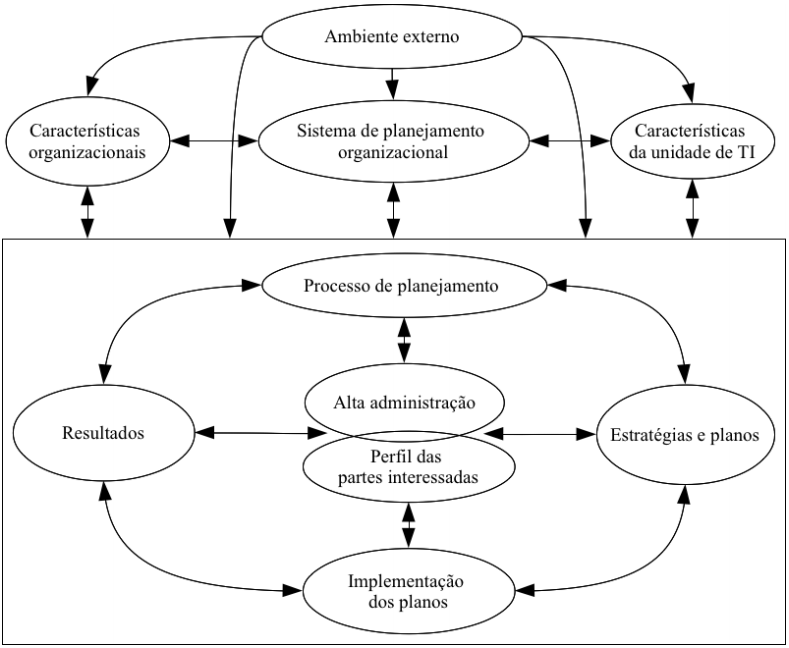
\includegraphics[width=14cm]{figuras/modeloBrown.png}
\caption{Modelo teórico de \citeonline{brown:04}, extraído de \citeonline{barros:13}}
\label{figura:modeloBrown}
\end{figure}

O modelo teórico de \citeonline{brown:04} exibe, através das categorias mapeadas na pesquisa, os conceitos que permeiam o planejamento de TI e suas relações. As categorias apresentadas neste modelo são:
\begin{itemize}
\item Ambiente externo;
\item Características organizacionais;
\item Sistema de planejamento organizacional;
\item Características da unidade de TI;
\item Processo de planejamento;
\item Resultados;
\item Alta administração;
\item Perfil das partes interessadas;
\item Estratégias e planos;
\item Implementação dos planos.
\end{itemize}


A presente pesquisa está inserida no contexto de organizações públicas. Desta forma, os modelos de planejamento voltados para organizações que disputam mercado podem não ser totalmente aplicáveis no cenário do setor público, apesar de apresentarem conceitos que podem ter correspondência no ambiente organizacional público. Diante disso, na seção seguinte são apresentados conceitos e abordagens de planejamento de TI voltados para obter eficiência e eficácia operacional, ou seja, objetivos mais aderentes à organizações públicas.

\section{Planejamento de TI no Setor Público}
% Luiza Página 27

% mundo
%ver minha revisão da literatura se tem nos artigos gringos umas referências sobre o planning na gringa

Espera-se de entidades públicas, que se dedicam à prestação de serviços públicos, o exercício das suas funções em níveis de qualidade comparáveis ao setor privado \cite{nezakati:14}. A denominação de planejamento de TI mais comum em bases acadêmicas estrangeiras é o planejamento de sistemas de informação (\textit{strategic information systems panning}). As agências estatais que se dedicam ao planejamento estratégico de sistemas de informação, de maneira formal e abrangente, são capazes de promover um ambiente mais favorável à utilização de TI dentro do governo \cite{bajjaly:98}. Casos de sucesso da aplicação de planejamento de TI no setor privado sugerem que adaptações nos modelos tradicionais de planejamento de TI podem preencher a lacuna entre os recursos estatais e as necessidades dos cidadãos \cite{dufner:02}.

% Can Private Sector Strategic Information Systems Planning Techniques Work for the Public Sector?
\citeonline{dufner:02} realizaram uma pesquisa com órgãos governamentais dos Estados Unidos e destacou que entidades do poder executivo e legislativo dos estados tinham baixo índice de envolvimento com planejamento de TI. Nesta pesquisa os autores buscam evidências de que o modelo criado para o planejamento estratégico de sistemas de informação é originalmente voltado para entidades privadas e vários fatores demandam adaptação no modelo para o setor público, por exemplo os objetivos organizacionais. A pesquisa de \citeonline{dufner:02} mostra que os objetivos organizacionais das empresas privadas abordam questões relacionadas à TI em suas metas, enquanto em empresas públicas a TI figura como uma ferramenta auxiliar e não como um componente importante para atingir os objetivos da organização. 

\citeonline{abu:09} traz um estudo sobre diferenças entre planejamento estratégico de sistemas de informação de empresas privadas e públicas, além de apresentar fatores de sucesso para um modelo de planejamento de TI voltado ao setor público. Em \citeonline{dufner:05}, os autores analisam quatro modelos de planejamento de TI utilizados em instituições públicas dos Estados Unidos. 

Com relação aos modelos de planejamento de TI para o setor público brasileiro, \citeonline{rezende:07} propôs uma metodologia para o planejamento de informação, conhecimento e informática para entidades públicas municipais. \citeonline{fagundes:11} propõe um modelo para elaboração do PDTI baseado em arquitetura corporativa e governança de TI. Em 2012, o Sistema de Administração dos Recursos de Tecnologia da Informação (SISP) do governo federal publicou a primeira versão do guia de elaboração do PDTI \cite{sisp:12}. %Na seção 3.3.4 deste trabalho são apresentados os principais modelos dedicados ao PDTI.

Assim como empresas privadas, os órgãos da administração pública necessitam planejar ações para atingir suas metas. A própria Constituição da República Federativa do Brasil de 1988, em seu artigo 174, declara que o Estado, como agente regulador da economia, exercerá a função de planejamento \cite{cf:88}. Na Administração Pública Federal o planejamento é um princípio fundamental estabelecido no Decreto Lei 200/1967. Desde 2008, através da Instrução Normativa 04/2008 \cite{in04:08} e da Estratégia Geral de Tecnologia da Informação \cite{egti:08}, os órgãos do poder executivo federal são obrigados a planejar as ações de TI através do PDTI. Portanto, todas as organizações públicas, devem desenvolver processos de planejamento e de monitoramento nos níveis institucionais e na área de TI \cite{tcuManual:07}.  

É importante que os órgãos públicos possuam planos, nos níveis estratégico, tático e/ou operacional, para as funções financeira, logística e de TI. O PETI, situado no nível estratégico, é um documento que complementa o Plano Estratégico Institucional, por meio do planejamento dos recursos de TI, possibilitando a definição de objetivos específicos para a área de TI. Ele estabelece as diretrizes e as metas que orientam a construção do planejamento de TI do órgão. Já no nível tático, o instrumento mais comumente usado para representar o planejamento de TI é o PDTI. O PDTI descreve de forma tática como uma organização, no que se refere à tecnologia da informação, pode realizar a transição de uma situação atual para uma situação futura, a partir da definição de um plano de metas e ações. No nível operacional, os planos de ação auxiliam a execução das ações e o alcance das metas, alinhados ao PDTI \cite{sisp:15}. 

É relevante compreender o fluxo dos processos de planejamento do governo federal brasileiro que se relacionam com os processos de planejamento de TI dos órgãos. O planejamento do governo é materializado em três instrumentos: Plano Plurianual (PPA), a Lei de Diretrizes Orçamentárias (LDO) e a Lei Orçamentária Anual (LOA). Os órgãos, por sua vez, tem como principal instrumento de planejamento o Planejamento Estratégico Institucional (PEI), alinhado aos planos superiores. Os setores de TI dos órgãos podem possuir o PETI e o PDTI como instrumentos de planejamento da área de tecnologia da informação, sendo que estes devem estar alinhados ao PEI \cite{sisp:15}. Segundo a IN 04/2014, ``inexistindo o plano estratégico institucional, sua ausência deverá ser registrada no PDTI e deverá ser utilizado um documento equivalente, como o Plano Plurianual'' \cite{in04:14}. A Figura \ref{figura:fluxoPlanejamentoGov} ilustra a relação dos instrumentos de planejamento de TI com os instrumentos de planejamento do governo.

\begin{figure}[h!]
\centering % para centralizarmos a figura
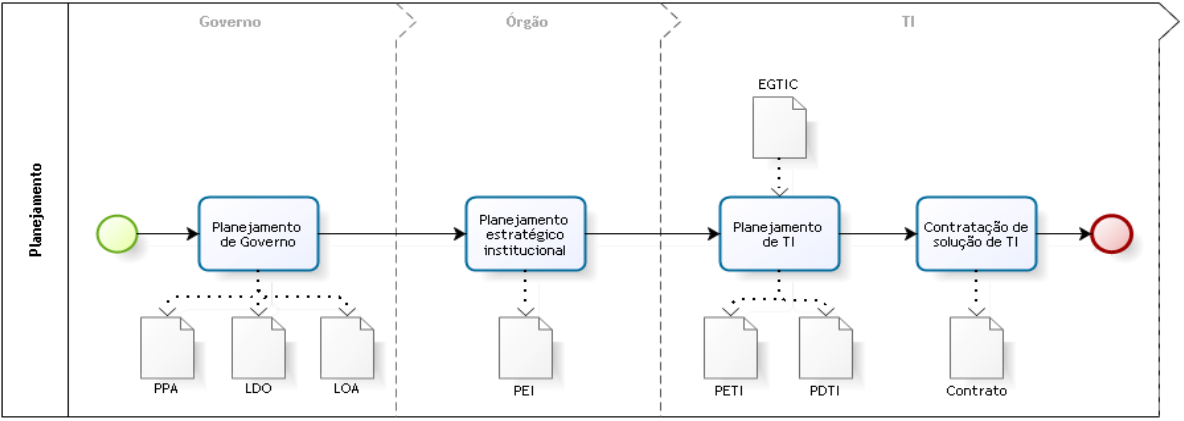
\includegraphics[width=14cm]{figuras/fluxoPlanejamentoGov.png}
\caption{Fluxo dos processos de planejamento de TI no governo brasileiro, extraído de \citeonline{sisp:15}.}
\label{figura:fluxoPlanejamentoGov}
\end{figure}

\subsection{IN 04/2008}

De acordo com balanço de compras públicas de 2014, o governo federal movimentou R\$6,03 bilhões com aquisições de bens e serviços de tecnologia da informação e comunicação \cite{balanco:14}. Isto evidencia que o setor público brasileiro é um grande cliente de serviços de TI. Segundo \citeonline{cruz:08}, ``o aumento na frequência de acórdãos e decisões do TCU relacionados no âmbito das contratações de serviços de TI, em especial a partir de 2002, indica maior preocupação do TCU com o tema e sugere a existência de problemas de gestão de contratação de serviços neste setor''. No Acórdão 786/2006 do TCU, itens 68 a 70 do voto do relator, são indicados recorrentes problemas em contratações de serviços de TI, além de críticas ao modelo de contratação da época:
\begin{citacao}
68.	Pode-se dizer que o modelo de contratação antes adotado pelo MDIC consistia na reunião de todos os serviços de informática do órgão em um único e grande contrato, adjudicado a uma única empresa, com pagamentos realizados por hora-trabalhada. 
69.	É necessário que se esclareça que essa prática, que equivale à contratação dos serviços de um CPD completo e terceirizado, não se restringia ao Ministério do Desenvolvimento, Indústria e Comércio Exterior. Em diversos processos examinados pelo Tribunal, verificou-se que foram muitos os casos em que licitações de serviços de informática vinham sendo promovidas pela Administração Pública Federal sem que se procedesse à divisão do objeto em parcelas, como preconizado pelo art. 23, §§ 1º e 2º, da Lei 8.666/93, apesar de tal alternativa se mostrar viável. A título de exemplo, podem ser citados certames realizados pelo Ministério do Planejamento (Concorrência 14/2000 - Decisão 1.067/2002 - Plenário), Agência Nacional do Cinema (Concorrência 02/2003 - Acórdão 1.937/203 - Plenário), Ministério da Educação (Concorrência 01/1999 - Acórdão 2.561/2004-2ª Câmara), Ministério da Justiça (Concorrência 03/2000 - Decisão 351/2002 - Plenário), entre outros.
70.	Esse modelo apresentava uma série de desvantagens potencialmente causadoras de prejuízos aos cofres públicos e à atividade da Administração. 
\end{citacao}

Diante de fatos desta natureza, o TCU recomendou, no mesmo acórdão (item 9.4), que Secretaria de Logística e Tecnologia da Informação (SLTI) do Ministério do Planejamento, Orçamento e Gestão elaborasse um modelo de licitação e contratação de serviços de TI para a APF:
\begin{citacao}
9.4. recomendar à Secretaria de Logística e Tecnologia da Informação do Ministério do Planejamento, Orçamento e Gestão que, a partir das diretrizes expostas na seção III do voto antecedente e nos Acórdãos deste Tribunal, sobretudo os de número 667/2005, 2.103/2005, 2.171/2005 e 2.172/2005, todos do Plenário, elabore um modelo de licitação e contratação de serviços de informática para a Administração Pública Federal e promova a implementação dele nos diversos órgãos e entidades sob sua coordenação mediante orientação normativa, que deve conter no mínimo:
9.4.1. a divisão dos serviços de informática necessários aos órgãos e entidades em tantos itens quanto sejam tecnicamente possíveis e suficientes;
9.4.2. a realização de licitação independente para cada item, contemplando requisitos de habilitação e critérios de avaliação de proposta técnica objetivos, relevantes e específicos para cada item, favorecendo assim a competitividade do certame, a redução de preços, a especialização das empresas, a qualidade dos serviços, a redução de riscos estratégicos e de segurança para o órgão ou entidade;
9.4.3. a mensuração, sempre que possível, da prestação de serviços por resultados segundo especificações previamente estabelecidas, evitando-se a mera locação de mão-de-obra e o pagamento por hora-trabalhada ou por posto de serviço, utilizando-se de metodologia expressamente definida no edital [...]
\end{citacao}

Fruto da recomendação do TCU, o Ministério do Planejamento, através da SLTI, publicou a instrução normativa número 4 (IN 04/2008) em 19 de maio de 2008 \cite{in04:08}. Este documento normatiza as contratações de serviços de TI na Administração Pública Federal direta, autárquica e fundacional. A IN 04/2008 é composta de três capítulos: Capítulo 1 - Disposições gerais; Capítulo 2 - Processo de contratação (capítulo composto de três seções -  planejamento da contratação, seleção de fornecedores e gerenciamento do contrato); Capítulo 3 - Disposições finais.

Nas disposições gerais, o documento traz o vínculo das contratações de serviços com o planejamento de TI nos órgãos da APF: ``Art. 3º As contratações de que trata esta Instrução Normativa deverão ser precedidas de planejamento, elaborado em harmonia com o Plano Diretor de Tecnologia da Informação - PDTI, alinhado à estratégia do órgão ou entidade''.

Ainda no primeiro capítulo da IN 04/2008, determina-se a criação da EGTI: ``Art. 4º Em consonância com o art. 4º do Decreto nº 1.048, de 1994, o órgão central do SISP elaborará, em conjunto com os órgãos setoriais e seccionais do SISP, a Estratégia Geral de Tecnologia da Informação para a Administração Pública, revisada anualmente, para subsídio à elaboração dos PDTI dos órgãos e entidades integrantes do SISP''.

Embora a IN 04/2008 tenha sido criada com a específica finalidade de disciplinar as contratações de serviços de TI, os artigos 3º e 4º apresentados anteriormente, evidenciam a importância desta normativa para a criação e consolidação de relevantes instrumentos de planejamento de TI no setor público brasileiro, como o PDTI e a EGTI. Em 2010 a IN 04 foi atualizada \cite{in04:10}, e a versão atual foi editada em 2014 \cite{in04:14}.


\subsection{EGTI e EGD}
%http://www.gestaoti.org/thesis/VladimirFagundes.pdf
A Estratégia Geral de Tecnologia da Informação foi criada em 2008 para vigorar em 2009. Seu objetivo foi estabelecer as bases para a transição entre a situação da gestão dos ambientes de TI do poder executivo federal da época - considerada heterogênea e vulnerável, conforme Acórdão 1603/2008 TCU Plenário - e o cumprimento da IN 04/2008 \cite{egti:08}. Desta forma, a primeira versão do documento apresenta um conjunto de metas para a melhoria da gestão de TI dos órgãos integrantes do SISP. Os órgãos deveriam apresentar um auto-diagnóstico e seus planejamentos para alcançar as metas, formalizando suas próprias trilhas de transição \cite{douEGTI:08}.

A EGTI de 2008 é composta de 4 seções:
\begin{enumerate}
\item \textbf{Apresentação:} são apresentados o objetivo do documento e o contexto que motivou a criação da EGTI.
\item \textbf{Princípios Norteadores:} faz referência aos princípios constitucionais; descreve a finalidade da aplicação dos recursos de TI no cumprimento da missão institucional do governo brasileiro, ressaltando a necessidade de planejamento em consonância com as metas institucionais; toma os \textit{frameworks} consagrados de Governança de TI como referência na elaboração de um modelo próprio.
\item \textbf{Modelo de Governança do SISP - Marco zero:} fornece as diretrizes para o início da elaboração do Modelo de Governança do SISP e delimita seu escopo organizado em grupos de práticas, sendo (i) aperfeiçoamento da gestão de TI e alinhamento estratégico; (ii) aprimoramento quali-quantitativo dos recursos humanos; (iii) melhoria do processo de contratação de TI; (iv) construção e adoção de padrões e modelos de gestão de TI; (v) segurança da informação; nesta seção é recomendado o auto-diagnóstico aos órgãos integrantes do SISP, para determinar suas respectivas posições na linha base do modelo de governança estabelecido.
\item \textbf{Sustentação ao Modelo de Governança do SISP:} são descritas as ações do SISP para apoiar os órgãos integrantes a cumprirem as metas de cada grupo de práticas.
\end{enumerate}

O PDTI é citado em diversos tópicos da EGTI desde a sua primeira versão. Na lista de metas para o ano de 2009, a existência e o uso efetivo de PDTI é pontuado no item 3.2.1.1. Outra meta descrita no documento é a elaboração do orçamento de TI com base nas ações planejadas no PDTI. No grupo de práticas relacionadas aos recursos humanos, a EGTI apresenta no item 3.2.2.1: ``Existência de quadro permanente em quantidade suficiente para gestão da área de TI e, em especial, para a elaboração e gestão do PDTI e dos processos de contratação'' \cite[p. 4]{egti:08}. A intenção de elaborar um modelo de referência do PDTI e oferecer cursos para a elaboração do plano também são abordados na EGTI de 2008.

A segunda versão da EGTI foi elaborada para ter vigência em 2010 \cite{egti:10}. Nesta versão houve uma revisão da EGTI anterior e apresentou os seguintes temas:
\begin{itemize}
\item Aperfeiçoamento da gestão de TI e alinhamento com planejamento institucional do órgão; 
\item Aprimoramento quali-quantitativo dos Recursos Humanos; 
\item Melhoria do Processo de Contratação de TI; 
\item Construção e Adoção de Padrões e Modelos de Apoio à Gestão e à Tecnologia; 
\item Gestão da Segurança da Informação; 
\item Gestão do SISP; 
\item Necessidade de alinhamento do PDTI à própria EG TI (conformidade estratégica).
\end{itemize}

A terceira versão da EGTI teve vigência no biênio 2011-2012 e buscou a continuidade da evolução das estratégias anteriores. Nesta versão o documento apresentou uma estrutura composta por 7 objetivos estratégicos, 18 metas e 56 iniciativas estratégicas, além de um plano de execução das ações a serem realizadas pelos órgãos integrantes \cite{egti:11}.

Na quarta versão da EGTI, o horizonte de vigência foi ampliado para três anos, contemplando o triênio 2013-2015. O documento pode ser sintetizado no compromisso de fortalecer a gestão e a governança estratégica, fazendo com que a estratégia definida seja sistematicamente implementada, acompanhada e analisada, para garantir que a visão de futuro e os objetivos planejados 
sejam alcançados. Nesta versão a estratégia foi alinhada ao Plano Plurianual 2012-2015 do governo federal, e ao Plano Brasil 2022 \cite{egti:13}. 

A quinta versão, rebatizada de Estratégia Geral de Tecnologia da Informação e Comunicações (EGTIC), foi lançada dentro do triênio da versão anterior, para vigorar nos anos de 2014 e 2015. A interrupção da quarta versão para o lançamento de uma nova estratégia em 2014 foi fruto do monitoramento estratégico que concluiu que era necessária uma revisão mais profunda para tornar o planejamento mais conciso e objetivo, além de alinhado às ações do governo \cite{egti:14}.

Em 2016 a EGTIC foi substituída pela Estratégia de Governança Digital (EGD). O Ministério do Planejamento, Orçamento e Gestão, em conjunto com o SISP, servidores públicos, especialistas, acadêmicos e cidadãos de modo geral, construiu a EGD que tem vigência de 4 anos (2016-2019). Este novo instrumento estratégico de TI têm respaldo na Política de Governança Digital - formalizada por meio do Decreto Presidencial nº 8.638, de 15 de janeiro de 2016.  A Estratégia foi publicada por meio da  Portaria nº 68, de 07 de março de 2016. 

\begin{citacao}
Governo digital refere-se ao uso de tecnologias digitais, como parte integrada das estratégias de modernização governamentais, para gerar benefícios para a sociedade. É baseado em um ecossistema governamental digital composto de atores de governo, empresas, organizações da sociedade civil e indivíduos que apoiam a produção e o acesso a dados, serviços e conteúdos mediante interações com o governo \cite{egd:16}.
\end{citacao}

A EGD possui 10 objetivos estratégicos divididos em 3 eixos: Acesso à informação; Prestação de serviços; Participação social. Para cada objetivo estratégico são traçados indicadores e metas, além de atividades denominadas iniciativas estratégicas, totalizando 51 iniciativas a serem realizadas pelos órgãos da APF \cite{egd:16}. Na Figura \ref{figura:egdDiagramaEstrategico}, são apresentados os objetivos estratégicos e os princípios que regem a EGD, sob a perspectiva da entrega de valor à sociedade.

\begin{figure}[h!]
\centering % para centralizarmos a figura
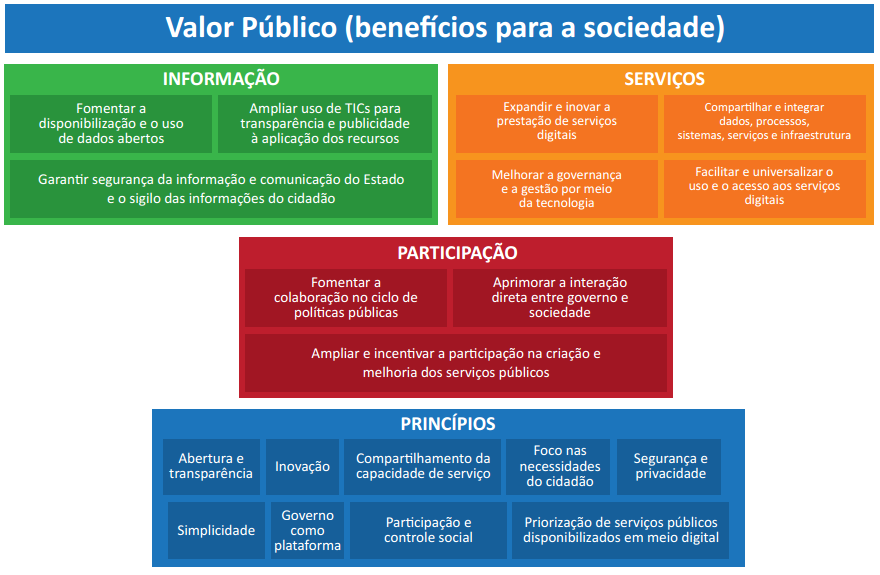
\includegraphics[width=14cm]{figuras/egdDiagramaEstrategico.png}
\caption{Diagrama estratégico da EGD, extraído de \cite{egd:16}.}
\label{figura:egdDiagramaEstrategico}
\end{figure}

Para o sucesso da EGD, os Planos Estratégicos Institucionais e os Planos Diretores de Tecnologia da Informação e Comunicação devem se alinhar aos objetivos e às iniciativas da EGD, conforme Figura \ref{figura:EGDalinhaPDTIC}. Para isto o documento recomenda aos órgãos da APF que incluam no conteúdo do PEI e do PDTIC (ou PDTI), metas e iniciativas que contribuam para o alcance dos objetivos da Estratégia de Governança Digital \cite{egd:16}.

\begin{figure}[h]
\centering % para centralizarmos a figura
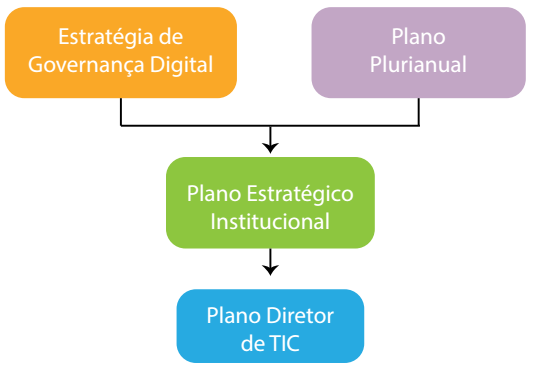
\includegraphics[width=6cm]{figuras/EGDalinhaPDTIC.png}
\caption{Integração da EGD com outras estratégias e planos, extraído de \cite{egd:16}.}
\label{figura:EGDalinhaPDTIC}
\end{figure}

O PDTIC, também chamado de PDTI, é apresentado na seção seguinte.

\subsection{PDTI}
% o que é
O planejamento de TI deve ser apresentado em um documento escrito, publicado e divulgado no âmbito da organização onde a área de TI atua \cite{sisp:12}. Para os órgãos integrantes do SISP\footnote{Sistema de Administração de Recursos de Tecnologia da Informação (SISP), organiza o planejamento, a coordenação, a organização, a operação, o controle e a supervisão dos recursos de TI dos órgãos e entidades da administração pública federal direta, autárquica e fundacional do poder executivo federal (Decreto no 7.579, de 11 de outubro de 2011).}, o planejamento de TI deve ser consolidado em um documento denominado Plano Diretor de Tecnologia da Informação. O PDTI é definido como um ``instrumento de diagnóstico, planejamento e gestão dos recursos e processos de Tecnologia da Informação que visa a atender às necessidades de informação de um órgão ou entidade para um determinado período'' \cite{in04:08,in04:10,in04:14}.

Segundo \citeonline{hazan:10}, o PDTI tem o objetivo de orientar uma organização no uso correto de seus recursos de TI, levando-a
focalizar nos processos de melhoria contínua de governança, além de atender aos princípios de racionalização, economicidade, uniformidade e padronização, criando as bases tecnológicas para a implantação com melhor eficiência e eficácia das políticas públicas. O PDTI representa um instrumento de gestão para a execução das ações e projetos de TI da organização, possibilitando justificar os recursos aplicados em TI, minimizar o desperdício e garantir o controle das atividades relacionadas à TI nos órgãos públicos da APF \cite{sisp:15}.

O PDTI ganha caráter obrigatório na IN 04/2008 quando explicita que as contratações de TI devem ser previstas no Plano: ``Art. 3º As contratações de que trata esta Instrução Normativa deverão ser precedidas de planejamento, elaborado em harmonia com o Plano Diretor de Tecnologia da Informação - PDTI, alinhado à estratégia do órgão ou entidade'' \cite{in04:08}. A existência e o uso efetivo do PDTI a partir de 2009, bem como a elaboração de um modelo de referência do Plano são abordados na primeira versão da EGTI \cite{egti:08}. 

% A inexistência de um PDTI pode causar um entendimento insuficiente do ambiente externo e interno da organização e de tecnologias emergentes que possam agregar valor aos serviços prestados aos clientes. Essa situação pode conduzir a investimentos inadequados em TI, considerando o atendimento às necessidades da organização para superar os seus desafios.  hazan:10

Considerando o caráter dinâmico do planejamento de TI devido ao fato da instabilidade dos ambientes tecnológicos, que estão em constante evolução, o PDTI deve ser anualmente revisado de forma que as estratégias estejam alinhadas à missão organizacional e à evolução da tecnologia \cite{hazan:10}.

\subsubsection{Modelos de PDTI}
%ordem cronlógica, please
Com a determinação de que os órgãos da Administração Pública Federal deveriam elaborar seus Planos Diretores de TI a partir de 2009, criou-se a necessidade de modelos e guias de orientação para a construção do PDTI. Em outubro de 2008, conforme previsto na primeira versão da EGTI, a SLTI publicou o primeiro modelo de referência de PDTI. Dividido em três fases - diagnóstico, planejamento e gestão - o modelo traz a estrutura básica do Plano. Além do modelo de referência, a SLTI propõe uma metodologia de elaboração do PDTI que será detalhada neste trabalho mais adiante.

\citeonline{fagundes:11} analisou dois modelos de PDTI aderentes à IN 04 e à EGTI naquela ocasião, em 2011, e propôs seu próprio modelo (PDGovTI). O primeiro modelo analisado por \citeonline{fagundes:11}, foi proposto pela empresa Microsoft em 2009, chamado Metodologia \textit{Microsoft Consulting Service} (MCS). O modelo tem conformidade com a IN 04, para isto segue orientações do \textit{framework} COBIT e de normas técnicas como a ISO/IEC 27002 e ISO/IEC 15999-1:2007. A metodologia MCS é distribuída sem custos para os órgãos públicos e é estruturada em cinco fases \cite{microsoft:09}:

\begin{itemize}
\item \textbf{Fase I:} Preparação e planejamento; Obter documentações; Inventariar TI; Elaborar diagnóstico de TI; Elaborar PETI.
\item \textbf{Fase II:} Pesquisar planos; Identificar setores-chave; Identificar responsáveis; Elaborar questionários de levantamento; Aplicar questionários; Consolidar levantamento de necessidades.
\item \textbf{Fase III:} Análise da situação desejada; Mapa de demandas futuras; Gerar mapa de demandas de TI.
\item \textbf{Fase IV:} Elaborar PDTI; Obter aprovação do Comitê de TI.
\item \textbf{Fase V:} Elaborar plano de execução do PDTI; Elaborar plano de monitoramento do PDTI.
\end{itemize}

O segundo modelo analisado por \citeonline{fagundes:11} também foi proposto no primeiro ano de obrigatoriedade do PDTI, em 2009. Trata-se de um modelo fornecido pela Escola Nacional de Administração Pública (ENAP) durante o curso de elaboração do PDTI de 2009. O modelo é baseado na IN 04/2008, no modelo de referência da SLTI e na EGTI \cite{cruz:08}. O modelo proposto no curso foi dividido em três etapas: preparação; diagnóstico da situação atual; planejamento da situação desejada.

Não existe uma determinação por parte do governo sobre qual modelo utilizar. Os órgãos membros do SISP são livres para seguir qualquer modelo ou criar os seus próprios, desde que atendam aos requisitos mínimos propostos na IN 04 e na EGD e, consequentemente, sejam alinhados às estratégias institucionais. Contudo, o modelo desenvolvido pela SLTI é destacado pelos órgãos membros do SISP, pois observa-se o comprometimento da SLTI em evoluir periodicamente o modelo de referência, assim como o processo de elaboração do Plano através do Guia de PDTI do SISP \cite{sisp:15}. Uma publicação que visa apoiar os órgãos a desenvolverem seus PDTI em conformidade com as normativas. Esta metodologia de elaboração do PDTI é detalhada na seção seguinte.

\subsubsection{Processo de elaboração do PDTI (Guia de PDTI do SISP)}
\label{secao:guia_pdti_sisp_cap3}
O processo de elaboração do PDTI apresentado nesta seção é descrito no Guia de PDTI do SISP, versão 2.0 beta \cite{sisp:15}. Seguindo a notação de modelagem de processos de negócio BPMN, mantida pela \textit{Object Management Group} (OMG), utiliza-se a hierarquia de elementos: macroprocessos, processos, subprocessos, atividades e tarefas.

O PDTI possui um ciclo de vida que se inicia com a criação do documento (processo de elaboração) e, após sua concepção deverá ser acompanhado ao longo de sua validade (processo de acompanhamento), realizando-se o monitoramento adequado que pode culminar em sua revisão. Um PDTI é finalizado com o término do seu período de validade e o Plano encerrado serve de insumo para o início da elaboração do Plano seguinte. Na Figura \ref{figura:pdti01Macroprocesso} é apresentado o macroprocesso do PDTI.

\begin{figure}[h!]
\centering % para centralizarmos a figura
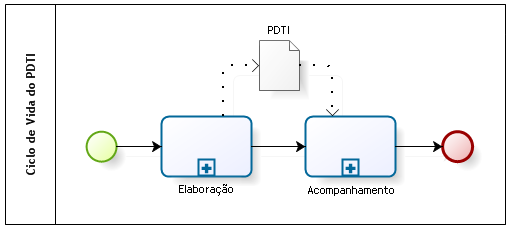
\includegraphics[width=10cm]{figuras/pdti01Macroprocesso.png}
\caption{Macroprocesso do PDTI, extraído de \cite{sisp:15}.}
\label{figura:pdti01Macroprocesso}
\end{figure}

Os principais papéis envolvidos no ciclo de vida do PDTI são:
\begin{itemize}
\item \textbf{Autoridade Máxima:} Membro da alta administração no nível hierárquico mais elevado da organização. É o principal patrocinador do PDTI e deverá prover recursos, tomar as decisões mais importantes, definir diretrizes gerais e tornar o PDTI público;
\item \textbf{Comitê de TI:} Requerido pela IN 04/2014, o comitê deve ser formado por representantes das áreas finalísticas e da TI da organização. Tem a prerrogativa de dirigir o alinhamento das ações e dos investimentos para o alcance dos objetivos estratégicos da organização, bem como priorizá-los, além de avaliar os resultados do desempenho da TI. O comitê é responsável pelo o atingimento dos objetivos e metas definidos no PDTI;
\item \textbf{Equipe de Elaboração do PDTI:} Grupo designado pelo Comitê de TI, formado por servidores tanto das áreas finalísticas quanto da TI. Equipe responsável por operacionalizar as atividades de elaboração do PDTI;
\item \textbf{Equipe de Acompanhamento do PDTI:} Equipe designada pelo Comitê de TI, responsável pelo acompanhamento do plano de ações do PDTI e pelo reporte dos resultados às partes interessadas. A equipe deve ser formada por servidores tanto das áreas finalísticas quanto da TI.
\end{itemize}

Três subprocessos compõem o processo de elaboração, sendo eles: preparação, diagnóstico e planejamento. O processo de elaboração é representado na Figura \ref{figura:pdti02Elaboracao}.
\begin{figure}[h!]
\centering % para centralizarmos a figura
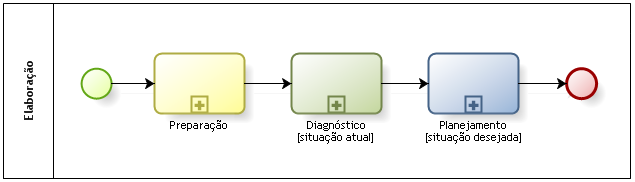
\includegraphics[width=12cm]{figuras/pdti02Elaboracao.png}
\caption{Processo de elaboração do PDTI, extraído de \cite{sisp:15}.}
\label{figura:pdti02Elaboracao}
\end{figure}

O subprocesso de preparação marca o início do processo de elaboração do PDTI. A primeira atividade consiste em definir a abrangência e o período de validade do PDTI, esta atividade deve ser realizada pelo comitê de TI. Em seguida o comitê deve definir a equipe de elaboração do PDTI e nomeá-los através de uma portaria de designação.

A primeira atividade da equipe de elaboração do PDTI no subprocesso de preparação é descrever a metodologia de elaboração do Plano. Em seguida a equipe deve produzir uma lista dos documentos de referência a serem utilizados no PDTI e listas contendo as estratégias organizacionais, princípios e diretrizes. Também é de responsabilidade da equipe de elaboração realizar nesta fase a primeira versão do inventário de necessidades. A última atividade da equipe de elaboração na fase de preparação é elaborar um plano de trabalho onde devem estar descritas as informações essenciais para organizar as atividades a serem desempenhadas durante o projeto de elaboração do PDTI. Cabe ao comitê de TI aprovar o plano de trabalho finalizando a fase de preparação.

Finalizada a preparação, inicia-se o subprocesso de diagnóstico que tem como objetivo analisar a situação atual da organização, resultando ao final do subprocesso no inventário de necessidades consolidado. Caso um PDTI necessite ser revisado, é nesta fase que a revisão deve iniciar.

Durante o diagnóstico da organização, a equipe de elaboração deve analisar os resultados do PDTI anterior, se houver; analisar o referencial estratégico de TI; analisar a organização da TI; realizar análise SWOT da TI; estimar a capacidade de execução da TI; planejar o levantamento de necessidades; identificar as necessidades de informação; identificar as necessidades de serviços, infraestrutura, contratação e pessoal de TI; consolidar o inventário de necessidades e alinhar cada necessidade de TI às estratégias da organização. Por fim, o comitê de TI aprova o inventário de necessidades finalizando a fase de diagnóstico.

Os subprocessos de preparação e diagnóstico servem de insumos para o subprocesso de planejamento, fase onde o PDTI é construído de fato. O planejamento é iniciado pelo comitê de TI com a atividade de atualização dos critérios de priorização à luz do conhecimento das necessidades levantadas anteriormente. A atividade seguinte é realizada pela equipe de elaboração e consiste na priorização das necessidades inventariadas.

Ainda no subprocesso de planejamento, a equipe de elaboração produz uma série de documentos que compõem o PDTI, sendo eles: Plano de Metas e Ações; Plano de Gestão de Pessoas; Plano Orçamentário; Lista dos fatores críticos de sucesso; Plano de Gestão de Riscos. A equipe de elaboração do PDTI encerra sua participação nesta fase consolidando uma minuta do PDTI que segue para a aprovação do comitê de TI e, por fim, para a autoridade máxima realizar a atividade de publicação do Plano. Desta forma o processo de elaboração do PDTI é finalizado. Todo o subprocesso de planejamento é ilustrado na Figura \ref{figura:pdti04Planejamento}.
\begin{figure}[h!]
\centering % para centralizarmos a figura
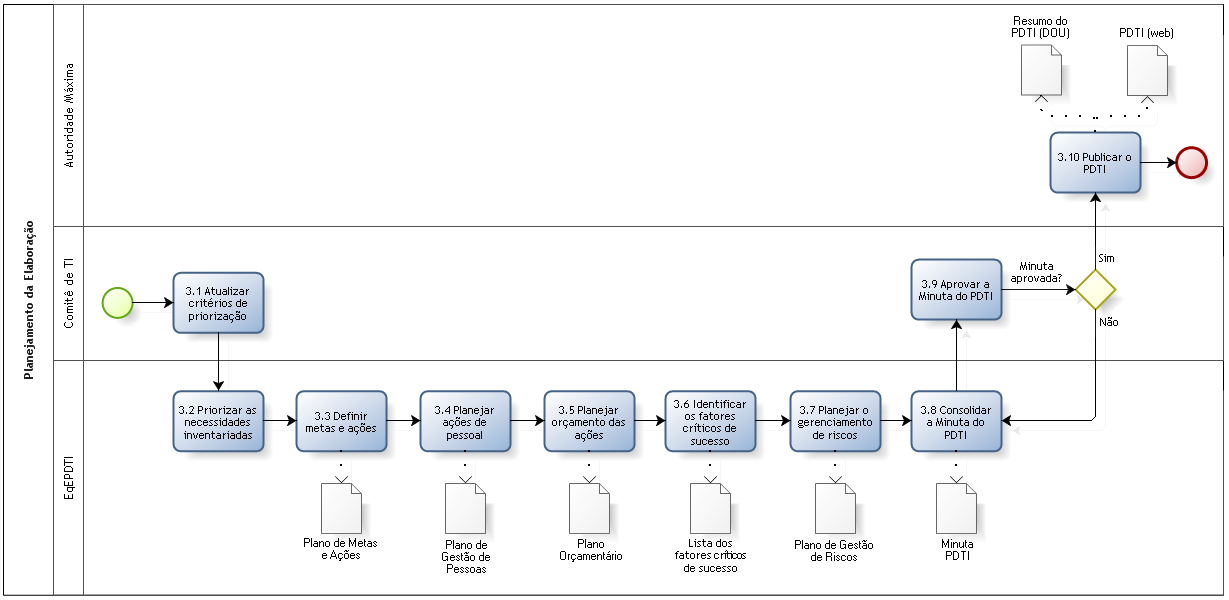
\includegraphics[width=16cm]{figuras/pdti04Planejamento.png}
\caption{Subprocesso de planejamento do PDTI, extraído de \cite{sisp:15}.}
\label{figura:pdti04Planejamento}
\end{figure}

\section{Trabalhos Relacionados}

%oportunidade de usar o trabalho de outros autores para motivar o seu próprio estudo

Inicialmente, é importante destacar que não há o objetivo de realizar um mapeamento sistemático da literatura neste trabalho. O intuito desta seção é apresentar trabalhos com temática diretamente relacionada a esta pesquisa. Os resultados das buscas por trabalhos relacionados foram classificados por relevância e selecionados informalmente, priorizando trabalhos recentes e com abordagens correlatas ao problema de pesquisa aqui apresentado.

Para buscar trabalhos relacionados ao tema foi utilizado o engenho de busca contido no Portal de Periódicos da CAPES, além da base de teses e dissertações. A Tabela \ref{tabela:stringsIngles} apresenta as \textit{strings} utilizadas nas buscas em língua inglesa e a Tabela \ref{tabela:stringsPortugues} apresenta as \textit{strings} utilizadas nas buscas em língua portuguesa. As buscas limitaram-se a trabalhos dos últimos seis anos, de 2011 a 2016.

% http://www.tablesgenerator.com/
% Please add the following required packages to your document preamble:
% \usepackage[table,xcdraw]{xcolor}
% If you use beamer only pass "xcolor=table" option, i.e. \documentclass[xcolor=table]{beamer}
\begin{table}[h!]
\centering
\begin{tabular}{|l|c|c|}
\hline
\rowcolor[HTML]{9B9B9B} 
\multicolumn{1}{|c|}{\cellcolor[HTML]{9B9B9B}{\color[HTML]{000000} \textit{\textbf{String}}}}                                    & {\color[HTML]{000000} \textbf{\begin{tabular}[c]{@{}c@{}}Trabalhos \\ retornados\end{tabular}}} & {\color[HTML]{000000} \textbf{\begin{tabular}[c]{@{}c@{}}Trabalhos\\ selecionados\end{tabular}}} \\ \hline
"IT Planning" (título)                                                                                                           & 7                                                                                               & 0                                                                                                \\ \hline
"Information Techonology Planning" (título)                                                                                      & 0                                                                                               & 0                                                                                                \\ \hline
\begin{tabular}[c]{@{}l@{}}"IT Planning" (título) AND \\ "government" (documento todo)\end{tabular}                              & 3                                                                                               & 0                                                                                                \\ \hline
\begin{tabular}[c]{@{}l@{}}"IT Planning" (título) AND \\ "Public Sector" (documento todo)\end{tabular}                           & 1                                                                                               & 0                                                                                                \\ \hline
"Strategic Information Systems Planning" (título)                                                                                & 15                                                                                              & 0                                                                                                \\ \hline
\begin{tabular}[c]{@{}l@{}}"Strategic Information Systems Planning" (título) \\ AND "government" (documento todo)\end{tabular}   & 5                                                                                               & 0                                                                                                \\ \hline
\begin{tabular}[c]{@{}l@{}}"Strategic Information Systems Planning" (título)\\ AND "public sector" (documento todo)\end{tabular} & 2                                                                                               & 0                                                                                                \\ \hline
\end{tabular}
\caption{\textit{Strings} de busca em periódicos na língua inglesa }
\label{tabela:stringsIngles}
\end{table}


% Please add the following required packages to your document preamble:
% \usepackage[table,xcdraw]{xcolor}
% If you use beamer only pass "xcolor=table" option, i.e. \documentclass[xcolor=table]{beamer}
\begin{table}[h!]
\centering
\begin{tabular}{|l|c|c|}
\hline
\rowcolor[HTML]{9B9B9B} 
\multicolumn{1}{|c|}{\cellcolor[HTML]{9B9B9B}{\color[HTML]{000000} \textit{\textbf{String}}}} & {\color[HTML]{000000} \textbf{\begin{tabular}[c]{@{}c@{}}Trabalhos \\ retornados\end{tabular}}} & {\color[HTML]{000000} \textbf{\begin{tabular}[c]{@{}c@{}}Trabalhos\\ selecionados\end{tabular}}} \\ \hline
"Planejamento de TI" (título) & 0 & 0 \\ \hline
"Planejamento de tecnologia da informação" (título) & 4 & 0 \\ \hline
"PDTI" (título) & 1 & 0 \\ \hline
"Plano diretor de TI" (título) & 1 & 0 \\ \hline
"Plano de TI" (título) & 0 & 0 \\ \hline
"Planos de TI" (título) & 1 & 1 \\ \hline
"Planejamento estratégico de TI" (título) & 13 & 0 \\ \hline
"Planejamento estratégico de\\ Tecnologia da Informação" (título) & 5 & 2 \\ \hline
\end{tabular}
\caption{\textit{Strings} de busca em trabalhos na língua portuguesa}
\label{tabela:stringsPortugues}
\end{table}

As buscas por trabalhos relacionados revelaram que a maior parte das produções acadêmicas sobre planejamento de TI se referem ao setor privado. Nos trabalhos mais recentes, das poucas publicações que abordam o planejamento de TI no setor público brasileiro a grande maioria são teses ou dissertações. O contrário ocorre com as publicações em língua inglesa, onde percebe-se que as publicações que abordam planejamento de TI no setor público são artigos de periódicos e conferências.

Na seleção dos trabalhos, o principal critério consistiu na relação entre o planejamento de TI e setor público. Posteriormente, foram filtrados apenas trabalhos focados em planejamentos de TI de organizações públicas brasileiras cujo escopo contribuísse para a presente pesquisa. Os três trabalhos relacionados são dissertações de mestrado: \citeonline{paula:12}; \citeonline{barros:13}; \citeonline{prando:15}.

\subsection{Fatores condicionantes relacionados ao planejamento de TI}
% do problema de pesquisa
A caracterização do problema na dissertação de \citeonline{paula:12} evidencia que naquela ocasião já era visível que, apesar da obrigatoriedade de realizar o planejamento de TI, os órgãos públicos brasileiros encontravam dificuldades para realizar tal atividade. Diante disso, \citeonline{paula:12} pesquisou sobre modelos de planejamento de TI aderentes ao setor público. Ao investigar as práticas de formulação e implantação do planejamento de TI em órgãos federais, \citeonline{barros:13} identificou fatores condicionantes que se relacionam com a formulação e implantação de planos de TI. No trabalho de \citeonline{prando:15}, um dos objetivos consiste em explorar as lacunas e conflitos presentes no processo de planejamento de TI de uma instituição pública federal em um cenário de expansão.

%dos fatores que dificultam o planejamento

\citeonline{paula:12} utilizou-se da literatura científica para levantar a hipótese de sua pesquisa. Nesta abordagem, a falta de um modelo de formulação de planejamento estratégico de TI voltado para instituições universitárias federais, seria o fator restritivo para que estas instituições atendessem satisfatoriamente o planejamento de TI. 

Para identificar os fatores condicionantes que influem na elaboração e execução dos planos de TI de órgãos públicos federais, \citeonline{barros:13} entrevistou dirigentes de TI codificando seus depoimentos de acordo com as categorias do modelo teórico de \citeonline{brown:04}. Desta forma, o autor organizou as percepções dos entrevistados a respeito do planejamento de TI sob a perspectiva das dez categorias do trabalho de \citeonline{brown:04}, que por sua vez, foram mapeadas a partir da literatura científica.

No trabalho de \citeonline{prando:15}, a pesquisa baseou-se em cinco proposições acerca das dificuldades relacionadas à elaboração do PDTI em uma determinada instituição. As proposições foram expostas à validação através de pesquisa documental, entrevistas e estudo de caso.

Um dos objetivos da presente pesquisa é identificar os fatores que dificultam ou impedem a elaboração do planejamento de TI em órgãos públicos federais. Desta forma, com o intuito de realizar comparações a Tabela \ref{tabela:fatoresTrabRelacionados} foi elaborada compilando os principais fatores que dificultam o planejamento de TI, sob a perspectiva de cada trabalho relacionado neste capítulo.

% Please add the following required packages to your document preamble:
% \usepackage{graphicx}
% \usepackage[table,xcdraw]{xcolor}
% If you use beamer only pass "xcolor=table" option, i.e. \documentclass[xcolor=table]{beamer}
\begin{table}[h!]
\centering
\resizebox{\textwidth}{!}{%
\begin{tabular}{|l|l|l|}
\hline
\rowcolor[HTML]{9B9B9B} 
\multicolumn{1}{|c|}{\cellcolor[HTML]{9B9B9B}{\color[HTML]{000000} Paula (2012)}}                                                      & \multicolumn{1}{c|}{\cellcolor[HTML]{9B9B9B}{\color[HTML]{000000} Barros (2013)}}                                                                                                                                                                                                                                                                                                                                                                                                                                                                                                                                                                                                                                                              & \multicolumn{1}{c|}{\cellcolor[HTML]{9B9B9B}{\color[HTML]{000000} Prando (2015)}}                                                                                                                                                                                                                                       \\ \hline
\begin{tabular}[c]{@{}l@{}}- Dificuldade em aplicar modelos de \\ planejamento de TI no cenário de instituição\\ pública.\end{tabular} & \begin{tabular}[c]{@{}l@{}}- Influência (negativa) da alta gestão;\\ - Mudanças no cenário político impedem o planejamento\\  a longo prazo;\\ - Contingenciamento orçamentário;\\ - Dificuldade em consolidar as informações de todas as \\ áreas em instituições com grande número de unidades;\\ - Rotatividade de dirigentes e descontinuidade \\ administrativa;\\ - Falta de governança corporativa;\\ - Falta de cultura de planejamento e de pensamento \\ estratégico;\\ - TI mal posicionada na hierarquia organizacional;\\ - Falta pessoal de TI;\\ - Falta qualificação do quadro de pessoal;\\ - Dificuldades para conseguir a participação das áreas\\ finalísticas;\\ - Dificuldades na priorização das demandas.\end{tabular} & \begin{tabular}[c]{@{}l@{}}- Expansão acelerada da instituição;\\ - Parte dos coordenadores de TI desconhecem\\ o PDTI;\\ - Alinhamento estratégico fraco ou inexistente;\\ - Coordenadores de TI há pouco tempo no cargo;\\ - Dificuldade em manter o comprometimento\\ dos participantes do comitê de TI.\end{tabular} \\ \hline
\end{tabular}%
}
\caption{Fatores que dificultam o planejamento de TI, segundo trabalhos relacionados.}
\label{tabela:fatoresTrabRelacionados}
\end{table}

Pode-se observar que dificuldades em aplicar modelos de planejamento de TI no setor público, como coloca \citeonline{paula:12}, não é um fator que aparece na teoria fundamentada nos dados apresentada nesta pesquisa. Isto permite inferir que os processos, guias e ferramentas disponíveis nas instituições pesquisadas não se apresentaram como dificuldade na elaboração do planejamento de TI.

Dos fatores citados no trabalho de \citeonline{barros:13} é possível observar que a influência (negativa) da alta gestão está presente nas duas teorias fundamentadas nos dados, assim como as deficiências de capacitação e quantitativas do pessoal de TI. A falta da cultura do planejamento, citada pelo autor, se faz presente na teoria 2 da presente pesquisa. Também foi citado por \citeonline{barros:13} o elemento centra da teoria 2: dificuldades com a participação das áreas finalísticas; desta forma corroborando com a teoria apresentada. Contudo, vários fatores citados pelo autor não se mostraram presentes nas teorias desta pesquisa, tais como: mudanças no cenário político, contingenciamento orçamentário, dificuldade em consolidar informações das unidades, rotatividade de dirigentes e dificuldade em priorizar as demandas.

Já no trabalho de \citeonline{prando:15} não foi possível traçar nenhuma relação direta entre os fatores levantados pelo autor e os elementos das teorias desta pesquisa. Porém, é possível inferir que há alguma relação entre o elemento central da teoria 2 (problemas na participação das áreas de negócio) com a dificuldade em manter o comprometimento dos participantes do comitê de TI, citado por \citeonline{prando:15}, uma vez que o comitê de TI deve conter membros de variadas áreas da instituição.

De forma geral, com exceção do trabalho de \citeonline{paula:12}, foi possível verificar que os trabalhos relacionados apontam para fatores condicionantes ao planejamento de TI de forma específica e pontual. As teorias apresentadas nesta pesquisa, conforme determina \citeonline{corbin:98}, são abrangentes o suficientes para englobar tais especifidades e se mostrou aderente em diversos fatores levantados nos trabalhos relacionados. Por outro lado, a teoria fundamentada nos dados desta pesquisa não revelou convergência com a maioria dos fatores listados pelos trabalhos relacionados apresentados nesta seção. Infere-se que os métodos de cada pesquisa possam influir nesta divergência parcial.

\subsection{Métodos utilizados}
Os métodos empregados em cada trabalho relacionado neste capítulo também contribuíram para a presente pesquisa. O intuito desta seção é destacar a metodologia de cada pesquisa para poder comparar os trabalhos e interpretar os resultados de forma ponderada. Desta maneira, não é objeto desta seção descrever os métodos, mas espera-se expor as características relevantes na influência dos resultados e suas análises.

\citeonline{paula:12} utilizou o método pesquisa-ação, que pode ser definida como ``toda tentativa continuada, sistemática e empiricamente fundamentada de aprimirar a prática'' \cite{tripp:05}. Neste cenário, a prática envolvida consiste na formulação do planejamento estratégico de TI de uma determinada instituição. A pesquisa-ação desenvolveu-se em três etapas: planejar, agir e refletir.

\begin{citacao}
Na etapa planejar, foi realizada a avaliação dos fatores que influenciam o planejamento estratégico de TI na UNIRIO e a análise dos modelos de planejamento estratégico de TI existentes na literatura. Na etapa Agir foi aplicado o Modelo de Planejamento Estratégico de TI desenvolvido pelo SISP, tendo como resultado o PDTIC da UNIRIO. Na etapa Refletir, foram apresentadas as reflexões sobre os efeitos decorrentes da aplicação da modelo do SISP e a identificação de possíveis melhorias para futuros ciclos de planejamento \cite{paula:12}.
\end{citacao}

No método utilizado por \citeonline{paula:12}, destaca-se a fase ``planejar'', na qual avaliou-se os fatores que influenciam o planejamento de TI da instituição. A autora confirmou seu problema de pesquisa nesta etapa ao traçar o cenário da instituição com relação ao planejamento de TI. Para isto, analisou o histórico da instituição; buscou a origem do problema de planejamento de TI estabelecendo contato com os participantes e interessados. Há de se destacar que a pesquisadora interferiu no ambiente da pesquisa por ser membro do comitê de TI da instituição pesquisada. Porém, o método utilizado permite tal interferência. Traçando um comparativo com a metodologia da presente pesquisa, a interferência do pesquisador não é bem-vinda, pois pode-se distanciar os dados da realidade e aproximá-los do viés do pesquisador.

A pesquisa de \citeonline{barros:13} é de natureza qualitativa, aplicando entrevistas semiestruturadas à alguns dirigentes de TI de organizações públicas federais. Os dados coletados são codificados de acordo com as categorias pré-concebidas no modelo teórico de \citeonline{brown:04}, ou seja, possui traços de \textit{Grounded Theory}. Desta forma, o pesquisador não apresenta uma teoria fundamentada nos dados, assim como foi apresentado no presente trabalho, mas uma classificação de códigos de acordo com um modelo teórico fundamentado na literatura.

\citeonline{prando:15} também optou pela abordagem qualitativa, porém utilizando os métodos de estudo de caso, entrevistas em profundidade e pesquisa documental. Tal metodologia permitiu ao pesquisador traçar o retrato fiel da instituição pesquisada e propor recomendações direcionadas aos problemas levantados. Porém, esta abordagem restringe a generalização do problema para outras instituições, uma vez que os fatores condicionantes levantados são de natureza específica da instituição em questão.

\subsection{Soluções propostas}
O trabalho de \citeonline{paula:12} permitiu a adaptação de um modelo de planejamento de TI existente, gerando um modelo exclusivo voltado para atender à instituição pesquisada. Desta forma, a pesquisadora buscou eliminar as lacunas e dificuldades que a instituição enfrentava no processo de elaboração do PDTI. Contudo, o contexto de outras instituições pode ser diferente e, com isto, o modelo proposto pode não ser aplicável.

A proposta de \citeonline{barros:13} é explorar a perspectiva dos dirigentes de TI e expor os fatores que influenciam a formulação e execução dos planos de TI. Os relatos dos dirigentes são ricos e o pesquisador os apresenta de forma a mostrar contrapontos e justificativas dos entrevistados. Porém, apesar de levantar os fatores condicionantes à elaboração do planejamento de TI, o trabalho não fornece uma proposta soluções aos problemas relacionados ao planejamento de TI. Ao contrário, a presente pesquisa propõe um conjunto de melhores práticas relacionadas aos fatores condicionantes.

A pesquisa de \citeonline{prando:15} oferece um conjunto de recomendações com o intuito de reduzir os problemas levantados. O autor não especifica a fonte das recomendações, desta forma infere-se que as sugestões foram baseadas no conhecimento do próprio autor. Por se tratar de uma pesquisa com foco específico em problemas de planejamento de TI de uma determinada instituição, fica dificultada a generalização das recomendações propostas e, consequentemente, a aplicação em outras instituições. As teorias apresentadas na presente pesquisa vão de encontro à abordagem de \citeonline{prando:15}, uma vez que apresenta uma teoria substancial e geral, além de apresentar uma proposta de solução com fundamentação nos dados.

\subsection{Considerações}
Os três trabalhos relacionados corroboram com a motivação da presente pesquisa fornecendo diferentes abordagens de identificação das dificuldades e deficiências no planejamento de TI de organizações públicas e propondo ações de melhoria para o cenário pesquisado.

A proposta da presente pesquisa, ao utilizar \textit{Grounded Theory}, não utilizou-se de premissas ou hipóteses assim como nos trabalhos de \citeonline{paula:12} e \citeonline{prando:15}. Ao contrário, as proposições foram levantadas na análise dos dados coletados e refutadas ou confirmadas também nos dados no desenvolver da pesquisa.

É interessante observar que \citeonline{barros:13} utilizou \textit{Grounded Theory} de forma indireta em sua pesquisa. Isto pode ser afirmado pois o autor codifica os dados utilizando categorias mapeadas anteriormente por \citeonline{brown:04}, que utilizaram GT para formular tal modelo. A criação das categorias da presente pesquisa foi feita de forma diferente, pois foram mapeadas a partir dos dados coletados exclusivamente para esta pesquisa, contribuindo para a fundamentação das teorias descobertas.

Os três trabalhos apresentados nesta pesquisa comungam de um problema prático presente nas instituições públicas brasileiras: as dificuldades em se planejar de forma eficaz as ações de TI de uma organização pública. As pesquisas aqui apresentadas apontam que a busca pela identificação dos fatores que levam a este problema é uma tarefa complexa e subjetiva. Porém, não atenderam a necessidade de compreender de forma abrangente os fatores limitadores do planejamento de TI e expor as relações causais entre estes limitadores. Tal lacuna foi sanada na presente pesquisa com duas teorias substanciais e abrangentes, ou seja, com fundamentação e genéricas o suficiente para aplicação em diversas organizações. A fundamentação empírica desta pesquisa é um diferencial para que a teoria reflita diretamente a prática, permitindo a proposição de soluções eficazes.

Por fim, esta pesquisa difere-se dos trabalhos relacionados também na proposta de solução do problema de planejamento de TI no setor público brasileiro. Apresentou-se as melhores práticas de planejamento estratégico de TI cujos resultados esperados atacam diretamente os elementos causais do problema pesquisado. Destaca-se ainda a utilização do método GT na fase de seleção das melhores práticas, mantendo o rigor científico e a fundamentação teórica da pesquisa.

%Porém, compreender a origem do problema é um passo necessário para propor as soluções.


\section{Considerações}
Este capítulo apresentou as bases teóricas sobre o alinhamento estratégico entre a TI e o negócio e sobre os principais instrumentos de planejamento de TI. Destacam-se as particularidades do planejamento de TI no setor público, além dos fatos e normativas que motivaram a evolução da gestão de TI nos órgãos públicos federais brasileiros.

Assim como no setor privado, existem diversos modelos de planejamento de TI para o setor público. É importante destacar o esforço que o governo federal têm feito, através da SLTI e dos órgãos da APF que compõem o SISP, ao desenvolver instrumentos como a Instrução Normativa número 4, a Estratégia Geral de TI e a Estratégia Geral Digital no intuito de prover as bases estratégicas para o amadurecimento da TI no âmbito do setor público.

O processo de elaboração do PDTI apresentado neste capítulo é utilizado por grande parte dos órgãos da APF e suas etapas serviram de insumo para a composição do questionário aplicado à amostragem de entes da administração pública durante esta pesquisa. 

Com o intuito de explorar a literatura científica sob à temática do planejamento de TI no setor público, o capítulo seguinte apresenta os trabalhos relacionados que possuem relevância no desenvolvimento da presente pesquisa.
%\chapter{Trabalhos Relacionados}
%oportunidade de usar o trabalho de outros autores para motivar o seu próprio estudo

Inicialmente, é importante destacar que não há o objetivo de realizar um mapeamento sistemático da literatura neste trabalho. O intuito deste capítulo é apresentar trabalhos com temática diretamente relacionada a esta pesquisa. Os resultados das buscas por trabalhos relacionados foram classificados por relevância e selecionados informalmente, priorizando trabalhos recentes e com abordagens correlatas ao problema de pesquisa aqui apresentado.

Para buscar trabalhos relacionados ao tema foi utilizado o engenho de busca contido no Portal de Periódicos da CAPES, além da base de teses e dissertações. A Tabela \ref{tabela:stringsIngles} apresenta as \textit{strings} utilizadas nas buscas em língua inglesa e a Tabela \ref{tabela:stringsPortugues} apresenta as \textit{strings} utilizadas nas buscas em língua portuguesa. As buscas limitaram-se a trabalhos dos últimos seis anos, de 2011 a 2016.

% http://www.tablesgenerator.com/
% Please add the following required packages to your document preamble:
% \usepackage[table,xcdraw]{xcolor}
% If you use beamer only pass "xcolor=table" option, i.e. \documentclass[xcolor=table]{beamer}
\begin{table}[h!]
\centering
\begin{tabular}{|l|c|c|}
\hline
\rowcolor[HTML]{9B9B9B} 
\multicolumn{1}{|c|}{\cellcolor[HTML]{9B9B9B}{\color[HTML]{000000} \textit{\textbf{String}}}}                                    & {\color[HTML]{000000} \textbf{\begin{tabular}[c]{@{}c@{}}Trabalhos \\ retornados\end{tabular}}} & {\color[HTML]{000000} \textbf{\begin{tabular}[c]{@{}c@{}}Trabalhos\\ selecionados\end{tabular}}} \\ \hline
"IT Planning" (título)                                                                                                           & 7                                                                                               & 0                                                                                                \\ \hline
"Information Techonology Planning" (título)                                                                                      & 0                                                                                               & 0                                                                                                \\ \hline
\begin{tabular}[c]{@{}l@{}}"IT Planning" (título) AND \\ "government" (documento todo)\end{tabular}                              & 3                                                                                               & 0                                                                                                \\ \hline
\begin{tabular}[c]{@{}l@{}}"IT Planning" (título) AND \\ "Public Sector" (documento todo)\end{tabular}                           & 1                                                                                               & 0                                                                                                \\ \hline
"Strategic Information Systems Planning" (título)                                                                                & 15                                                                                              & 0                                                                                                \\ \hline
\begin{tabular}[c]{@{}l@{}}"Strategic Information Systems Planning" (título) \\ AND "government" (documento todo)\end{tabular}   & 5                                                                                               & 0                                                                                                \\ \hline
\begin{tabular}[c]{@{}l@{}}"Strategic Information Systems Planning" (título)\\ AND "public sector" (documento todo)\end{tabular} & 2                                                                                               & 0                                                                                                \\ \hline
\end{tabular}
\caption{\textit{Strings} de busca em periódicos na língua inglesa }
\label{tabela:stringsIngles}
\end{table}


% Please add the following required packages to your document preamble:
% \usepackage[table,xcdraw]{xcolor}
% If you use beamer only pass "xcolor=table" option, i.e. \documentclass[xcolor=table]{beamer}
\begin{table}[h!]
\centering
\begin{tabular}{|l|c|c|}
\hline
\rowcolor[HTML]{9B9B9B} 
\multicolumn{1}{|c|}{\cellcolor[HTML]{9B9B9B}{\color[HTML]{000000} \textit{\textbf{String}}}} & {\color[HTML]{000000} \textbf{\begin{tabular}[c]{@{}c@{}}Trabalhos \\ retornados\end{tabular}}} & {\color[HTML]{000000} \textbf{\begin{tabular}[c]{@{}c@{}}Trabalhos\\ selecionados\end{tabular}}} \\ \hline
"Planejamento de TI" (título) & 0 & 0 \\ \hline
"Planejamento de tecnologia da informação" (título) & 4 & 0 \\ \hline
"PDTI" (título) & 1 & 0 \\ \hline
"Plano diretor de TI" (título) & 1 & 0 \\ \hline
"Plano de TI" (título) & 0 & 0 \\ \hline
"Planos de TI" (título) & 1 & 1 \\ \hline
"Planejamento estratégico de TI" (título) & 13 & 0 \\ \hline
"Planejamento estratégico de\\ Tecnologia da Informação" (título) & 5 & 2 \\ \hline
\end{tabular}
\caption{\textit{Strings} de busca em trabalhos na língua portuguesa}
\label{tabela:stringsPortugues}
\end{table}

As buscas por trabalhos relacionados revelaram que a maior parte das produções acadêmicas sobre planejamento de TI se referem ao setor privado. Nos trabalhos mais recentes, das poucas publicações que abordam o planejamento de TI no setor público brasileiro a grande maioria são teses ou dissertações. O contrário ocorre com as publicações em língua inglesa, onde percebe-se que as publicações que abordam planejamento de TI no setor público são artigos de periódicos e conferências.

Na seleção dos trabalhos, o principal critério de seleção consistiu na relação entre o planejamento de TI e setor público. Posteriormente, foram filtrados apenas trabalhos focados em planejamentos de TI de organizações públicas brasileiras cujo escopo contribuísse para a presente pesquisa. Os três trabalhos relacionados são dissertações de mestrado: \citeonline{paula:12}; \citeonline{barros:13}; \citeonline{prando:15}.

\section{Fatores Condicionantes Relacionados ao Planejamento de TI}
% do problema de pesquisa
A caracterização do problema na dissertação de \citeonline{paula:12} evidencia que naquela ocasião já era visível que, apesar da obrigatoriedade de realizar o planejamento de TI, os órgãos públicos brasileiros encontravam dificuldades para realizar tal atividade. Diante disso, \citeonline{paula:12} pesquisou sobre modelos de planejamento de TI aderentes ao setor público. Ao investigar as práticas de formulação e implantação do planejamento de TI em órgãos federais, \citeonline{barros:13} identificou fatores condicionantes que se relacionam com a formulação e implantação de planos de TI. No trabalho de \citeonline{prando:15}, um dos objetivos consiste em explorar as lacunas e conflitos presentes no processo de planejamento de TI de uma instituição pública federal em um cenário de expansão.

%dos fatores que dificultam o planejamento

\citeonline{paula:12} utilizou-se da literatura científica para levantar a hipótese de sua pesquisa. Nesta abordagem, a falta de um modelo de formulação de planejamento estratégico de TI, voltado para instituições universitárias federais, seria o fator restritivo para que estas instituições atendessem satisfatoriamente o planejamento de TI. 

Para identificar os fatores condicionantes que influem na elaboração e execução dos planos de TI de órgãos públicos federais, \citeonline{barros:13} entrevistou dirigentes de TI codificando seus depoimentos de acordo com as categorias do modelo teórico de \citeonline{brown:04}. Desta forma, o autor organizou as percepções dos entrevistados a respeito do planejamento de TI sob a perspectiva das dez categorias do trabalho de \citeonline{brown:04}, que por sua vez, foram mapeadas a partir da literatura científica.

No trabalho de \citeonline{prando:15}, a pesquisa baseou-se em cinco proposições acerca das dificuldades relacionadas à elaboração do PDTI em uma determinada instituição. As proposições foram expostas à validação através de pesquisa documental, entrevistas e estudo de caso.

Um dos objetivos deste trabalho é identificar os fatores que dificultam ou impedem a elaboração do planejamento de TI em órgãos públicos federais. Desta forma, com o intuito de realizar comparações após os resultados da pesquisa, a Tabela \ref{tabela:fatoresTrabRelacionados} foi elaborada compilando os principais fatores que dificultam o planejamento de TI, sob a perspectiva de cada trabalho relacionado neste capítulo.

% Please add the following required packages to your document preamble:
% \usepackage{graphicx}
% \usepackage[table,xcdraw]{xcolor}
% If you use beamer only pass "xcolor=table" option, i.e. \documentclass[xcolor=table]{beamer}
\begin{table}[h!]
\centering
\resizebox{\textwidth}{!}{%
\begin{tabular}{|l|l|l|}
\hline
\rowcolor[HTML]{9B9B9B} 
\multicolumn{1}{|c|}{\cellcolor[HTML]{9B9B9B}{\color[HTML]{000000} Paula (2012)}}                                                      & \multicolumn{1}{c|}{\cellcolor[HTML]{9B9B9B}{\color[HTML]{000000} Barros (2013)}}                                                                                                                                                                                                                                                                                                                                                                                                                                                                                                                                                                                                                                                              & \multicolumn{1}{c|}{\cellcolor[HTML]{9B9B9B}{\color[HTML]{000000} Prando (2015)}}                                                                                                                                                                                                                                       \\ \hline
\begin{tabular}[c]{@{}l@{}}- Dificuldade em aplicar modelos de \\ planejamento de TI no cenário de instituição\\ pública.\end{tabular} & \begin{tabular}[c]{@{}l@{}}- Influência (negativa) da alta gestão;\\ - Mudanças no cenário político impedem o planejamento\\  a longo prazo;\\ - Contingenciamento orçamentário;\\ - Dificuldade em consolidar as informações de todas as \\ áreas em instituições com grande número de unidades;\\ - Rotatividade de dirigentes e descontinuidade \\ administrativa;\\ - Falta de governança corporativa;\\ - Falta de cultura de planejamento e de pensamento \\ estratégico;\\ - TI mal posicionada na hierarquia organizacional;\\ - Falta pessoal de TI;\\ - Falta qualificação do quadro de pessoal;\\ - Dificuldades para conseguir a participação das áreas\\ finalísticas;\\ - Dificuldades na priorização das demandas.\end{tabular} & \begin{tabular}[c]{@{}l@{}}- Expansão acelerada da instituição;\\ - Parte dos coordenadores de TI desconhecem\\ o PDTI;\\ - Alinhamento estratégico fraco ou inexistente;\\ - Coordenadores de TI há pouco tempo no cargo;\\ - Dificuldade em manter o comprometimento\\ dos participantes do comitê de TI.\end{tabular} \\ \hline
\end{tabular}%
}
\caption{Fatores que dificultam o planejamento de TI, segundo trabalhos relacionados.}
\label{tabela:fatoresTrabRelacionados}
\end{table}

\section{Métodos Utilizados}
Os métodos empregados em cada trabalho relacionado neste capítulo também contribuem para a presente pesquisa. O intuito desta seção é destacar a metodologia de cada pesquisa para poder comparar os trabalhos e interpretar os resultados de forma ponderada. Desta maneira, não é objeto desta seção descrever os métodos, mas espera-se expor as características relevantes na influência dos resultados e suas análises.

\citeonline{paula:12} utilizou o método pesquisa-ação, que pode ser definida como ``toda tentativa continuada, sistemática e empiricamente fundamentada de aprimirar a prática'' \cite{tripp:05}. Neste cenário, a prática envolvida consiste na formulação do planejamento estratégico de TI de uma determinada instituição. A pesquisa-ação desenvolveu-se em três etapas: planejar, agir e refletir.

\begin{citacao}
Na etapa planejar, foi realizada a avaliação dos fatores que influenciam o planejamento estratégico de TI na UNIRIO e a análise dos modelos de planejamento estratégico de TI existentes na literatura. Na etapa Agir foi aplicado o Modelo de Planejamento Estratégico de TI desenvolvido pelo SISP, tendo como resultado o PDTIC da UNIRIO. Na etapa Refletir, foram apresentadas as reflexões sobre os efeitos decorrentes da aplicação da modelo do SISP e a identificação de possíveis melhorias para futuros ciclos de planejamento \cite{paula:12}.
\end{citacao}

No método utilizado por \citeonline{paula:12}, destaca-se a fase ``planejar'', na qual avaliou-se os fatores que influenciam o planejamento de TI da instituição. A autora confirmou seu problema de pesquisa nesta etapa ao traçar o cenário da instituição com relação ao planejamento de TI. Para isto, analisou o histórico da instituição; buscou a origem do problema de planejamento de TI estabelecendo contato com os participantes e interessados. Há de se destacar que a pesquisadora interferiu no ambiente da pesquisa por ser membro do comitê de TI da instituição pesquisada. Porém, o método utilizado permite tal interferência.

A pesquisa de \citeonline{barros:13} é de natureza qualitativa, aplicando entrevistas semiestruturadas à alguns dirigentes de TI de organizações públicas federais. Os dados coletados são codificados de acordo com as categorias pré-concebidas no modelo teórico de \citeonline{brown:04}, ou seja, possui traços de \textit{Grounded Theory}. Desta forma, o pesquisador não apresenta uma teoria fundamentada nos dados, mas uma classificação de códigos de acordo com um modelo teórico fundamentado na literatura.

\citeonline{prando:15} também optou pela abordagem qualitativa, porém utilizando os métodos de estudo de caso, entrevistas em profundidade e pesquisa documental. Tal metodologia permitiu ao pesquisador traçar o retrato fiel da instituição pesquisada e propor recomendações direcionadas aos problemas levantados. Porém, esta abordagem restringe a generalização do problema para outras instituições, uma vez que os fatores condicionantes levantados são de natureza específica da instituição em questão.

\section{Soluções Propostas}
O trabalho de \citeonline{paula:12} permitiu a adaptação de um modelo de planejamento de TI existente, gerando um modelo exclusivo voltado para atender à instituição pesquisada. Desta forma, a pesquisadora buscou eliminar as lacunas e dificuldades que a instituição enfrentava no processo de elaboração do PDTI. Contudo, o contexto de outras instituições pode ser diferente e, com isto, o modelo proposto pode não ser aplicável.

A abordagem do trabalho de \citeonline{barros:13} não tem como objetivo propor soluções aos problemas relacionados ao planejamento de TI. A proposta é explorar a perspectiva dos dirigentes de TI e expor os fatores que influenciam a formulação e execução dos planos de TI. Os relatos dos dirigentes são ricos e o pesquisador os apresenta de forma a mostrar contrapontos e justificativas dos entrevistados.

A pesquisa de \citeonline{prando:15} oferece um conjunto de recomendações com o intuito de reduzir os problemas levantados. O pesquisador não especifica a fonte das recomendações, desta forma infere-se que as sugestões foram baseadas no conhecimento do próprio pesquisador. Por se tratar de uma pesquisa com foco específico em problemas de planejamento de TI de uma determinada instituição, fica dificultada a generalização das recomendações propostas e, consequentemente, a aplicação em outras instituições.

\section{Considerações}
Os três trabalhos relacionados corroboram com a motivação da presente pesquisa fornecendo abordagens de identificação das dificuldades e deficiências no planejamento de TI de organizações públicas e propondo ações de melhoria para o cenário pesquisado.

A proposta da presente pesquisa, ao utilizar \textit{Grounded Theory}, não utiliza-se de premissas ou hipóteses assim como nos trabalhos de \citeonline{paula:12} e \citeonline{prando:15}. Ao contrário, as proposições são levantadas na análise dos dados coletados e refutadas ou confirmadas também nos dados no desenvolver da pesquisa.

É interessante observar que \citeonline{barros:13} utilizou \textit{Grounded Theory} de forma indireta em sua pesquisa. Isto pode ser afirmado pois o autor codifica os dados utilizando categorias mapeadas anteriormente por \citeonline{brown:04}, que utilizaram GT para formular tal modelo. A criação das categorias da presente pesquisa foi feita de forma diferente, pois foram mapeadas a partir dos dados coletados exclusivamente para esta pesquisa.

Os três trabalhos apresentados nesta pesquisa comungam de um problema prático presente nas instituições públicas brasileiras: as dificuldades em se planejar de forma eficaz as ações de TI de uma organização pública. As pesquisas aqui apresentadas apontam que a busca pela identificação dos fatores que levam a este problema é uma tarefa complexa e subjetiva. Porém, ainda se faz necessário compreender de forma abrangente os fatores limitadores do planejamento de TI e expor as relações causais entre estes limitadores. Espera-se sanar esta necessidade com uma teoria abrangente, ou seja, genérica o suficiente para aplicação em diversas organizações; e com fundamentação empírica para que a teoria reflita diretamente a prática, permitindo a proposição de soluções eficazes.

%Porém, compreender a origem do problema é um passo necessário para propor as soluções. %virou seção do cap de considerações finais (novo cap6)
\chapter{Análise dos Problemas de Planejamento de TI em Instituições Públicas Brasileiras}
\label{capitulo:analise_dos_problemas}
Ao buscar os fatores que influenciam nas deficiências dos planejamentos de TI de instituições públicas, esta pesquisa adquire caráter multidisciplinar. Apesar de ser uma atividade vinculada aos ativos de tecnologia, o planejamento é um instrumento essencial da administração e absorve a subjetividade do comportamento dos indivíduos participantes. Neste cenário, o método de pesquisa qualitativa \textit{Grounded Theory} é empregado para analisar o problema e extrair resultados fundamentados na realidade.

\citeonline{glaser:68} apontam alguns pontos fortes da \textit{Grounded Theory}: (i) a fundamentação de dados empíricos  aproxima a pesquisa da realidade; (ii) por se tratar de análise de comportamento, é um método efetivo para o estudo do comportamento humano; (iii) possibilita novas perspectivas, pois toma a realidade como referencial teórico ao invés de buscar fundamentação em teorias já existentes.

Cabe aqui relembrar a questão que este trabalho busca responder: ``apesar da obrigatoriedade e dos conhecidos benefícios, o planejamento de TI não é realizado satisfatoriamente nos órgãos públicos federais. A atividade de planejamento envolve aspectos técnicos e sociais, diante disso, pergunta-se: quais os fatores que dificultam o processo de elaboração do planejamento de TI e qual a relação entre tais fatores?''.

Este capítulo tem como objetivo principal narrar o processo de coleta, análise, descoberta dos resultados e avaliação dos mesmos. Destaca-se a aplicação do método \textit{Grounded Theory} na fase de análise dos dados que, por sua natureza, deve ser capaz de fornecer as evidências para auditorias da pesquisa, arguições e reprodução do caminho percorrido pelo pesquisador até os resultados \cite{corbin:98}.

\section{Coleta dos Dados}
%https://goo.gl/rVPuFK

A amostragem de instituições públicas federais tomada para a aplicação do questionário de coleta de dados, representado no \autoref{apendice:a_quest_coleta}, consiste em Universidades Federais (UFs) e Institutos Federais de Educação, Ciência e Tecnologia (IFs). Na época da aplicação do \textit{survey}, o país contava com um total de 63 UFs e 41 IFs. A presente pesquisa contou com a participação de membros de 37 instituições, representando 35,57\% das instituições federais de ensino superior e técnico.

O público alvo ao qual se destinou o questionário é composto de servidores das instituições da amostragem que participaram de equipes de elaboração do PDTI, comitês de TI ou que atuaram como gestores de setores de TI. O total de respondentes do \textit{survey} soma 53 participantes. Para as análises qualitativas, 4 respostas foram descartadas, pois os respondentes deixaram as questões dissertativas em branco. Os dados foram separados em dois grupos, conforme segue:
\begin{itemize}
\item \textbf{Grupo 1 (instituições sem PDTI):} 9 respostas válidas.
\item \textbf{Grupo 2 (instituições com PDTI):} 40 respostas válidas;
\end{itemize}

Em um total de 53 participantes, o gráfico abaixo apresenta a proporção dos cargos efetivos dos servidores participantes da coleta de dados.

\begin{figure}[h]
\centering % para centralizarmos a figura
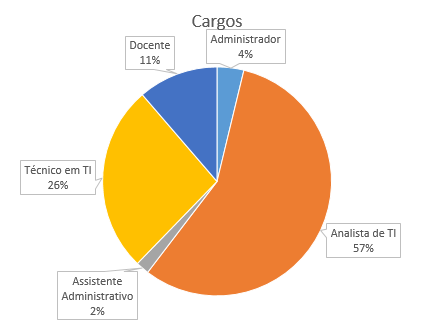
\includegraphics[width=9cm]{figuras/apendiceC_cargos.png}
%\caption{Cargos dos respondentes.}
\end{figure}

Dos 53 participantes, 34 possuem cargo de confiança.

Com relação ao tempo na instituição (em anos), os participantes se distribuem da seguinte forma:
\begin{itemize}
\item 2 anos ou menos: 9 participantes;
\item 3 a 5 anos: 22 participantes;
\item 6 a 10 anos: 14 participantes;
\item 10 a 20 anos: 5 participantes;
\item 20 anos ou mais: 3 participantes.
\end{itemize}

Com relação à formação acadêmica, os participantes estão distribuídos da seguinte forma:
\begin{figure}[h]
\centering % para centralizarmos a figura
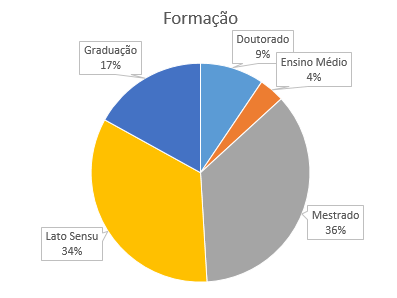
\includegraphics[width=9cm]{figuras/apendiceC_formacao.png}
%\caption{Formação dos respondentes.}
\end{figure}

A Tabela \ref{tabela:resumoColeta} apresenta um resumo da participação no questionário de coleta de dados.

% Please add the following required packages to your document preamble:
% \usepackage{graphicx}
% \usepackage[table,xcdraw]{xcolor}
% If you use beamer only pass "xcolor=table" option, i.e. \documentclass[xcolor=table]{beamer}
\begin{table}[]
\centering
\resizebox{\textwidth}{!}{%
\begin{tabular}{|l|c|c|c|}
\hline
\rowcolor[HTML]{9B9B9B} 
\multicolumn{1}{|c|}{\cellcolor[HTML]{9B9B9B}\textbf{Instituição}} & \textbf{Possui PDTI} & \textbf{Número de respondentes} & \textbf{Respostas válidas} \\ \hline
CEFET-MG                                                           & Sim                  & 1                               & 1                          \\ \hline
IFB                                                                & Sim                  & 1                               & 1                          \\ \hline
IFC                                                                & Sim                  & 7                               & 6                          \\ \hline
IFES                                                               & Sim                  & 1                               & 1                          \\ \hline
IF Farroupilha                                                     & Sim                  & 1                               & 0                          \\ \hline
IFG                                                                & Não                  & 1                               & 1                          \\ \hline
IF Goiano                                                          & Sim                  & 1                               & 1                          \\ \hline
IFMA                                                               & Sim                  & 2                               & 2                          \\ \hline
IFMT                                                               & Sim                  & 3                               & 3                          \\ \hline
IFPE                                                               & Não                  & 2                               & 2                          \\ \hline
IFPI                                                               & Não                  & 2                               & 1                          \\ \hline
IFPR                                                               & Sim                  & 1                               & 1                          \\ \hline
IFRO                                                               & Sim                  & 1                               & 1                          \\ \hline
IFRS                                                               & Sim                  & 1                               & 1                          \\ \hline
IFS                                                                & Sim                  & 1                               & 1                          \\ \hline
IFSC                                                               & Sim                  & 3                               & 3                          \\ \hline
IF Sudeste MG                                                      & Sim                  & 3                               & 3                          \\ \hline
UFAL                                                               & Sim                  & 1                               & 1                          \\ \hline
UFC                                                                & Sim                  & 1                               & 1                          \\ \hline
UFERSA                                                             & Sim                  & 1                               & 1                          \\ \hline
UFFS                                                               & Sim                  & 1                               & 1                          \\ \hline
UFGD                                                               & Sim                  & 1                               & 1                          \\ \hline
UFJF                                                               & Sim                  & 1                               & 0                          \\ \hline
UFOB                                                               & Não                  & 1                               & 1                          \\ \hline
UFPA                                                               & Não                  & 1                               & 1                          \\ \hline
UFPB                                                               & Sim                  & 1                               & 1                          \\ \hline
UFPE                                                               & Sim                  & 1                               & 1                          \\ \hline
UFRGS                                                              & Sim                  & 1                               & 1                          \\ \hline
UFRPE                                                              & Sim                  & 1                               & 1                          \\ \hline
UFRR                                                               & Não                  & 1                               & 1                          \\ \hline
UFS                                                                & Sim                  & 1                               & 1                          \\ \hline
UFSJ                                                               & Não                  & 1                               & 1                          \\ \hline
UFSM                                                               & Sim                  & 2                               & 2                          \\ \hline
UFTM                                                               & Sim                  & 1                               & 1                          \\ \hline
UFTO                                                               & Sim                  & 1                               & 1                          \\ \hline
UNIFESSPA                                                          & Não                  & 1                               & 1                          \\ \hline
UTFPR                                                              & Sim                  & 1                               & 1                          \\ \hline
\end{tabular}%
}
\caption{Instituições participantes da pesquisa.}
\label{tabela:resumoColeta}
\end{table}

O questionário foi elaborado levando em consideração a existência de instituições que possuem o PDTI, enquanto outras não possuem. A plataforma eletrônica escolhida para a aplicação do \textit{survey} permitiu o direcionamento do respondente para as questões de acordo com a situação do PDTI de sua instituição. O processo de elaboração do PDTI descrito no ``Guia do PDTI'' do SISP, orientou a ordem e o conteúdo das questões.

O grupo 1 possui apenas uma questão dissertativa: ``Quais os impedimentos ou dificuldades que a gestão de TI da sua instituição encontrou que justifique a falta de um PDTI?''. Os respondentes produziram o material de análise do grupo 1 ao responder a este questionamento.

O grupo 2 possui cinco questões dissertativas, como segue abaixo:
\begin{itemize}
\item A respeito do diagnóstico das necessidades de TI da instituição, fale sobre as dificuldades encontradas durante o processo de levantamento de necessidades na sua instituição;
\item Fale sobre as dificuldades encontradas na elaboração de critérios e priorização das necessidades da sua instituição;
\item Fale sobre as dificuldades encontradas na etapa de definição de metas e ações;
\item Fale sobre as dificuldades encontradas na etapa de planejar o gerenciamento de riscos;
\item Comente sobre qualquer outra dificuldade que tenha chegado ao seu conhecimento que a equipe que participou da elaboração ou revisão do PDTI tenha enfrentado.
\end{itemize}

O questionário é composto de questões objetivas e dissertativas sobre a elaboração do Plano Diretor de TI nas respectivas instituições dos respondentes. As questões objetivas tem o intuito de informar dados sobre os participantes, além de fornecer parâmetros quantitativos sobre o tema pesquisado, como pode ser visualizado no relatório do \autoref{apendice:c_relat_quantitativo}. As questões dissertativas, foco desta pesquisa, tem o objetivo de coletar os relatos dos participantes sobre suas experiências com o PDTI. Estas respostas, presentes no \autoref{apendice:d_respostas_disserta}, são os dados de entrada para a etapa de análise descrita na seção seguinte.

\section{Análise: Aplicação do Método Grounded Theory}

\begin{citacao}
Embora não criemos dados, criamos teoria a partir dos dados. Se fizermos isso corretamente, então não estaremos falando para nossos participantes, mas, sim, permitindo que eles falem com vozes claramente entendidas e representativas. Nossas teorias, embora imcompletas, fornecem uma linguagem comum (conjunto de conceitos) por meio da qual participantes da pesquisa, profissionais e outros podem se reunir para discutir ideias e encontrar soluções para os problemas \cite{corbin:98}.
\end{citacao}

Para analisar os dados, principalmente nas fases iniciais do método, utilizou-se da técnica de microanálise\footnote{Análise detalhada dos dados coletados, linha por linha ou palavra por palavra, necessária no começo de um estudo para gerar as primeiras categorias \cite{corbin:98}.}. Esta técnica consiste em buscar significado em pequenas porções dos dados, frases ou até mesmo palavras, de forma isolada do restante do texto. \citeonline{corbin:98} sugere que o pesquisador pergunte: ``O que esta palavra parece significar, ou o que ela poderia significar?''. Este exercício permite que o pesquisador busque por significados fora dos modos usuais, tornando-o consciente do quanto está contido em pequenas quantias de dados.

A microanálise evita que se tome partido ou que se assuma uma posição em relação aos dados. O pesquisador, desta forma, é forçado a pensar fora do senso comum e, com isso, o dado se mantém isolado sem ser forçado a assumir um conceito baseado em contexto. As falsas suposições ou significados atribuídos inicialmente sobre os dados não se sustentam, pois os dados são confrontados e comparados uns com os outros na medida em que se avança a análise \cite{corbin:98}.

As subseções seguintes tem o objetivo de narrar a análise dos dados coletados utilizando as fases da \textit{Grounded Theory} como arcabouço. Esta etapa da pesquisa, objetivando ser fiel ao método GT, buscou referências em livros textos e trabalhos acadêmicos acerca do método. As referências utilizadas para a aplicação do método de análise foram \citeonline{strauss:87}, \citeonline{corbin:98}, \citeonline{bandeira:03}, \citeonline{conte:09} e \citeonline{schots:10}.

	\subsection{Codificação aberta}
	
\citeonline{corbin:98} definem a codificação aberta como um processo analítico através do qual conceitos são identificados nos dados e suas propriedades e dimensões são descobertas. Nesta etapa trabalha-se com a ideia de 
códigos. ``Um código representa um conceito que dá significado a um trecho do documento, podendo se referir a uma citação, objeto, evento, problema, aspecto ou situação'' \cite{schots:10}.

O primeiro passo tomado na codificação aberta é a leitura completa do material coletado, que no caso desta pesquisa trata-se de um conjunto de respostas no formato texto, conforme apresentado no \autoref{apendice:d_respostas_disserta}. A leitura inicial permite uma visão geral do material de análise.

Os autores de \textit{Grounded Theory} indicam eleger um documento base após a leitura inicial, ou seja, um documento mais completo, mais rico em conceitos \cite{strauss:87,corbin:98}. O objetivo desta atividade é estabelecer os primeiros códigos que, posteriormente, ganharão densidade ao serem observados nos demais documentos. No caso desta pesquisa, há apenas um documento para cada grupo de análise. Diante disso, optou-se por começar a codificação pelas respostas mais completas, mais ricas em conceitos em cada um dos grupos. No grupo 1, a análise iniciou pela resposta cujo identificador é ID-3. Já no grupo 2, foi eleita a resposta de identificador ID-9 da primeira questão. Ambas respostas são transcritas a seguir.

\textit{\textbf{Grupo 1, resposta ID-3:} ``Falta de iniciativa e incentivo da alta gestão; Falta de plano estratégico institucional objetivo; Falta de pessoal voltado especificamente a área de planejamento e governança''.}

\textit{\textbf{Grupo 2, questão 1, resposta ID-9:} ``O inventário de necessidades é realizado por equipes nos Campi e Reitoria. No geral, encontram-se dificuldades em se estabelecer reuniões objetivas com os clientes do negócio. Muitas vezes os mesmos superestimam as necessidades dado algum receio de que não haja ``outra oportunidade''  para comprar bens e serviços em TI. Também é difícil ter que fazer compreender que as necessidades devem estar alinhadas aos objetivos estratégico e não desejos dos usuários''.}

Ao aplicar a técnica de microanálise nos dados citados acima, originaram-se os primeiros códigos. A resposta ID-3, por exemplo, originou os seguintes códigos: ``Falta PEI'', ``Alta gestão imatura'', ``Falta de iniciativa'', ``Falta de incentivo'' e ``Falta equipe especialista''.

Para cada código gerado, foi redigido um comentário descrevendo as características do conceito que representa tal código. Além disso, o comentário contém os critérios que permitam a uma citação ser candidata a se ligar a este código. Por exemplo, o comentário do código ``Alta gestão imatura''  apresenta o seguinte conteúdo:

\textit{\textbf{Código - Alta gestão imatura:}
Conceito que se refere a imaturidade estratégica da cúpula administrativa de uma instituição. Setor ligado à alta administração, tomadores de decisões estratégicas da instituição.
Este código pode ser aplicado em situações onde os dados façam referência à deficiência estratégica por parte da reitoria e/ou pró-reitorias. Os setores de TI não estão inclusos neste conjunto.}

Os comentários de todos os códigos desta pesquisa são apresentados no \autoref{apendice:e_codigos}.

Durante o processo de microanálise na busca por códigos, são feitos questionamentos aos dados e comparações teóricas com situações semelhantes para que haja uma minuciosa examinação e interpretação dos dados. Isto permite melhor compreensão do conceito e faz com que as propriedades e dimensões dos códigos emerjam dos dados \cite{corbin:98}. Tais questionamentos e comparações feitas foram registradas em notas (\textit{memos}), que nesta fase, são chamadas de notas de microanálise (MA). Também deve constar nos \textit{memos} MA, toda a descrição do processo de validação dos questionamentos e proposições buscando citações no formulário analisado ou nos demais, trata-se da fundamentação nos dados. Abaixo, um exemplo de uma nota do tipo MA:

\textit{\textbf{MA Códigos ``Falta de iniciativa''  e ``Falta de incentivo'': }}
\textit{
estes códigos parecem significar que falta de iniciativa e/ou de incentivo são causas para a falta de um PDTI. Quem deveria tomar esta iniciativa? Este tipo de resposta seria uma transferência de culpa? Deixa a sensação de que se houvesse o ``primeiro passo'', o PDTI teria acontecido. A alta gestão não incentiva a criação do PDTI, será que esta instituição não recebeu recomendações do TCU ou orientações do SISP que fomentam o ``incentivo'' à criação do PDTI?
Fundamentação: a citação do respondente ID3 indica que quem deveria tomar a iniciativa e incentivar seria a alta gestão da instituição, ou seja, a iniciativa não é da própria equipe de TI e o incentivo deve partir da alta gestão. 
O respondente do ID23, cita que há cobranças de órgãos de controle, isto é um ``incentivo'' a se criar o PDTI.}

Todas as notas de microanálise desta pesquisa são apresentadas no \autoref{apendice:f_notas_ma}.

O documento base serviu para registrar os primeiros códigos. O processo de codificação, incluindo as anotações de comentários e microanálise, foi aplicado nas demais respostas fazendo comparações com aquelas já analisadas e com os novos códigos registrados de forma recursiva. O processo de codificação, apesar de ser descrito de forma sequencial neste trabalho, ocorre de forma iterativa, conforme ilustra a Figura \ref{figura:gt_iterativo}.

\begin{figure}[h]
\centering % para centralizarmos a figura
\includegraphics[width=15cm]{figuras/gt_iterativo.png}
\caption{Processo de análise, extraído de \citeonline{bandeira:03}.}
\label{figura:gt_iterativo}
\end{figure}

Nesta etapa da codificação aberta a pesquisa apresenta: (i) a validação de códigos criados anteriormente; (ii) incremento do número de citações relacionadas a um determinado código; (iii) a criação de novos códigos. Uma vez que os códigos vão se acumulando, inicia-se o processo de agrupamento dos códigos ou categorização dos mesmos sob termos mais abstratos, isto é, categorias. A categoria representa um fenômeno observado a partir dos dados e responde a perguntas do tipo ``O que está acontecendo?'' \cite{corbin:98}.

Para encontrar as categorias, os códigos e anotações criados anteriormente foram revistos, analisando aqueles que possuem propriedades em comum que permitam elevar o nível de abstração do fenômeno ali representado, originando categorias. Em um exemplo hipotético apresentado por \citeonline{corbin:98}, os códigos “pássaro”, “pipa” e “avião” possuem uma propriedade em comum, que é a habilidade de voar e, desta forma, podem ser agrupados na categoria “voa”.

As categorias precisam ser descritas em função de suas propriedades e dimensões para facilitar o retorno aos dados, ou seja, servem como critérios para procurar outros códigos que se relacionam com aquela categoria. Propriedade é um atributo da categoria que, em conjunto com outras propriedades, dão significado à categoria. Já a dimensão se trata de uma métrica ou conjunto de valores que uma determinada propriedade da categoria pode assumir \cite{strauss:87}.

Um exemplo de categoria mapeada no grupo 1 é a categoria ``Deficiências na gestão da instituição''. Esta categoria possui a propriedade ``nível de maturidade em gestão na instituição'' que, por sua vez, possui duas dimensões: alta e baixa, onde a primeira indica instituição com indicadores positivos de maturidade na gestão e a segunda, com indicadores negativos de maturidade na gestão. Todos os códigos que tem esta propriedade são candidatos a fazerem parte da categoria.

No grupo 2, um exemplo de categoria mapeada é a categoria ``Problemas com recursos humanos'', cuja propriedade é o ``grau de adequação dos recursos humanos para as atividades de planejamento de TI''. As dimensões para a propriedade desta categoria são: adequado (recursos humanos adequados para as atividades do PDTI) e inadequado (recursos humanos inadequados para as atividades do PDTI).

O conjunto completo das categorias levantadas nesta pesquisa é apresentado no \autoref{apendice:e_codigos}. Após a criação das categorias, retorna-se ao material, explorando-as e fazendo novos questionamentos em busca de detalhar as categorias em subcategorias. Ao final da codificação aberta, é possível observar o mapa de códigos e categorias criados nesta primeira fase de codificação. Tais códigos e categorias estão sujeitos a sofrerem alterações nas fases seguintes da análise. As Figuras \ref{figura:oc_grupo1} e \ref{figura:oc_grupo2} representam o esquema teórico de códigos no momento da conclusão da codificação aberta dos grupos 1 e 2, respectivamente.

\begin{figure}[h]
\centering % para centralizarmos a figura
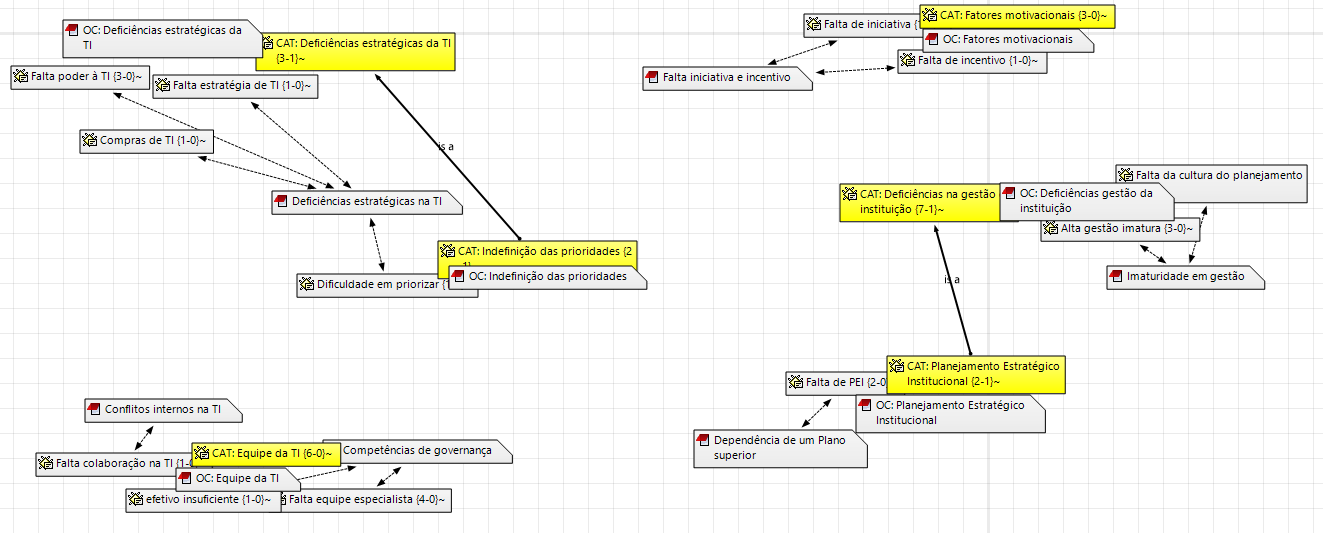
\includegraphics[width=16cm, frame]{figuras/oc_grupo1.PNG}
\caption{Esquema teórico do grupo 1 após a codificação aberta.}
\label{figura:oc_grupo1}
\end{figure}

\begin{figure}[h]
\centering % para centralizarmos a figura
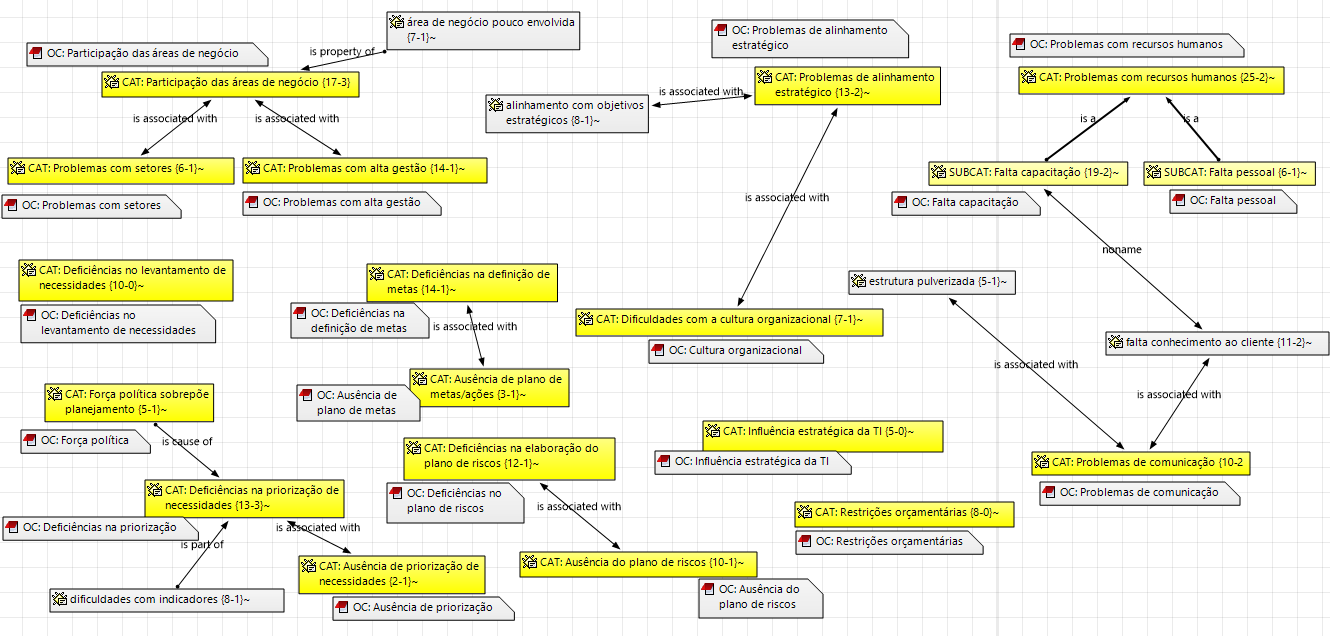
\includegraphics[width=16cm, frame]{figuras/oc_grupo2.PNG}
\caption{Esquema teórico do grupo 2 após a codificação aberta.}
\label{figura:oc_grupo2}
\end{figure}
	
Foram criadas notas de codificação aberta (OC), para cada categoria, contendo as citações que se encaixam em cada dimensão de cada propriedade. As notas do tipo OC também podem conter a narração do processo de retorno aos dados descrevendo os \textit{insights} e quaisquer questionamentos ou interpretações julgadas importantes para registrar o caminho de pensamento que levou a enquadrar determinada citação em determinada propriedade. A Figura \ref{figura:oc_memo} apresenta um trecho de uma das notas do tipo OC da presente pesquisa. 

\begin{figure}[h]
\centering % para centralizarmos a figura
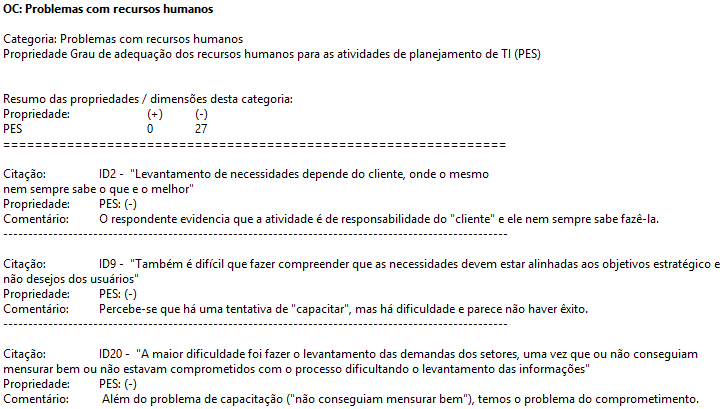
\includegraphics[width=16cm, frame]{figuras/oc_memo.PNG}
\caption{Exemplo de nota de codificação aberta.}
\label{figura:oc_memo}
\end{figure}

Pode-se observar, inclusive que a nota de codificação aberta possui a quantidade de ocorrências de cada dimensão de cada propriedade. Todas as notas do tipo OC podem ser observadas no \autoref{apendice:h_notas_oc}.

Ao final da codificação aberta as categorias estão com propriedades bem definidas e padrões de ocorrência efetivamente encontrados nos dados. Propriedades que não encontraram fundamentação empírica são descartadas e, com isto, categorias também podem ser alteradas ou excluídas. Isto garante a fundamentação empírica.

	\subsection{Codificação axial}
A codificação axial pode ser resumida no processo de relacionar categorias entre si e entre subcategorias. O termo “axial” é usado pois, uma a uma, a categoria é posta em um eixo de análise onde o objetivo é relacioná-la ao nível de propriedades e dimensões \cite{corbin:98}.

De acordo com \citeonline{corbin:98}, começando com análises das primeiras respostas, o pesquisador não deve ajudar, mas observar (e fazer anotações) como os códigos se relacionam. Ao explicar os relacionamentos, cria-se ligações entre categorias e suas subcategorias. Este procedimento permite verificar se os relacionamentos parecem ser condições, ações/interações ou consequências. Estes três elementos formam o que os autores chamam de paradigma \cite{conte:09}. Aos palpites iniciais formados por paradigmas, dá-se o nome de hipóteses ou proposições, pois eles ligam dois ou mais conceitos, explicando o que, porquê, onde, e como do fenômeno.

Na prática, esta etapa consiste em analisar uma categoria por vez, buscando relacionar com suas subcategorias identificando os códigos que representam condições, ações/interações e consequências. Para isso, é interessante ``quebrar'' a categoria em questão expondo seus códigos (propriedades, dimensões e subcategorias). As ligações entre cada código foram rotuladas, seguindo uma convenção de conectores, conforme apresentado na \autoref{secao:principios_da_gt}.

Após mapear os relacionamentos categorias-subcategorias de todas as categorias, o mesmo processo foi aplicado para mapear os relacionamentos entre categorias. Sempre que identificado um relacionamento, os \textit{insights}, os questionamentos e a lógica de pensamento que estruturou o relacionamento foram relatados em anotações, nesta etapa, chamadas de notas de codificação axial (AC). 

Há uma nota do tipo AC para cada relacionamento e nela contém proposições, ou hipóteses que passam por validação nos dados. As hipóteses foram estruturadas usando os elementos: condições, ações/interações e consequências. Após a criação de todos relacionamentos, com suas respectivas notas do tipo AC, retornou-se aos dados para buscar nos formulários de respostas evidências que dão veracidade à cada hipótese descrita nas anotações. Todas as notas AC desta pesquisa são apresentadas no \autoref{apendice:i_notas_ac}. A Figura \ref{figura:ac_memo} ilustra uma destas anotações.

\begin{figure}[h!]
\centering % para centralizarmos a figura
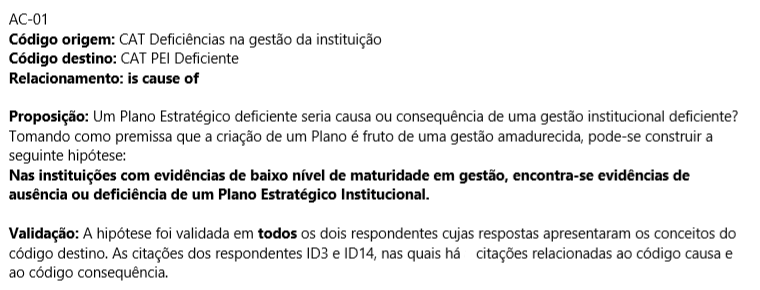
\includegraphics[width=16cm, frame]{figuras/ac_memo.PNG}
\caption{Exemplo de nota de codificação axial.}
\label{figura:ac_memo}
\end{figure}

As Figuras \ref{figura:ac_grupo1} e \ref{figura:ac_grupo2} representam o esquema teórico com as categorias e seus relacionamentos, no momento da conclusão da codificação axial dos grupos 1 e 2, respectivamente.

\begin{figure}[!ht]
\centering % para centralizarmos a figura
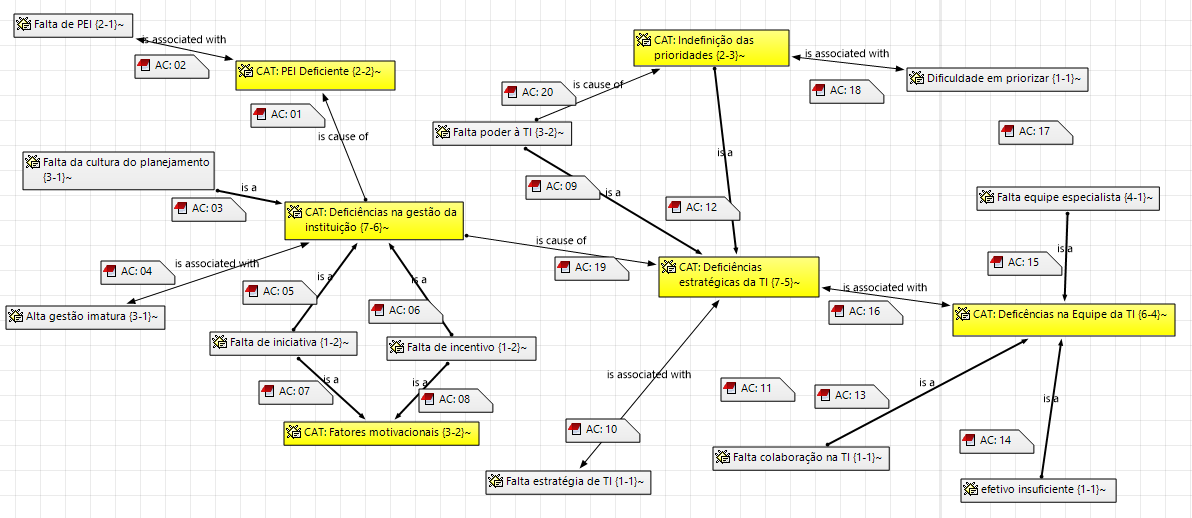
\includegraphics[width=16cm, frame]{figuras/ac_grupo1.PNG}
\caption{Esquema teórico do grupo 1 após a codificação axial.}
\label{figura:ac_grupo1}
\end{figure}

\begin{figure}[!ht]
\centering % para centralizarmos a figura
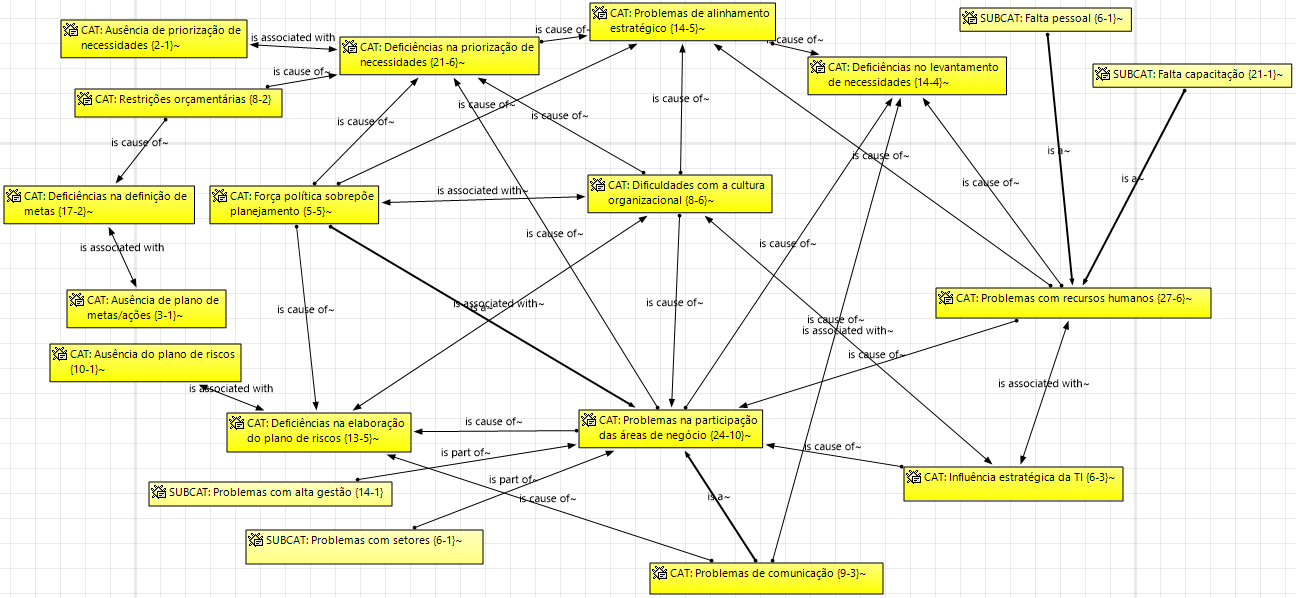
\includegraphics[width=16cm, frame]{figuras/ac_grupo2.PNG}
\caption{Esquema teórico do grupo 2 após a codificação axial.}
\label{figura:ac_grupo2}
\end{figure}

As Tabelas \ref{tabela:relacionamentos_teoria1} e \ref{tabela:relacionamentos_teoria2} apresentam os relacionamentos entre as categorias ao final da etapa de codificação axial.

\begin{table}[H]
\centering
\resizebox{\textwidth}{!}{%
\begin{tabular}{|
>{\columncolor[HTML]{C0C0C0}}l |l|l|l|l|}
\hline
\multicolumn{1}{|c|}{\cellcolor[HTML]{C0C0C0}\textbf{Categoria}}                 & \multicolumn{1}{c|}{\cellcolor[HTML]{C0C0C0}\textbf{is a}}                 & \multicolumn{1}{c|}{\cellcolor[HTML]{C0C0C0}\textbf{is cause of}}                               & \multicolumn{1}{c|}{\cellcolor[HTML]{C0C0C0}\textbf{is associated with}}   & \multicolumn{1}{c|}{\cellcolor[HTML]{C0C0C0}\textbf{is part of}} \\ \hline
PEI Deficiente                                                                   &                                                                            &                                                                                                 &                                                                            &                                                                  \\ \hline
\begin{tabular}[c]{@{}l@{}}Deficiências na \\ gestão da instituição\end{tabular} &                                                                            & \begin{tabular}[c]{@{}l@{}}PEI Deficiente;\\ \\ Deficiências \\ estratégicas da TI\end{tabular} &                                                                            &                                                                  \\ \hline
Fatores motivacionais                                                            &                                                                            &                                                                                                 &                                                                            &                                                                  \\ \hline
\begin{tabular}[c]{@{}l@{}}Indefinição das \\ prioridades\end{tabular}           & \begin{tabular}[c]{@{}l@{}}Deficiências \\ estratégicas da TI\end{tabular} &                                                                                                 &                                                                            &                                                                  \\ \hline
\begin{tabular}[c]{@{}l@{}}Deficiências \\ estratégicas da TI\end{tabular}       &                                                                            &                                                                                                 & \begin{tabular}[c]{@{}l@{}}Deficiências \\ na equipe da TI\end{tabular}    &                                                                  \\ \hline
\begin{tabular}[c]{@{}l@{}}Deficiências\\ na equipe da TI\end{tabular}           &                                                                            &                                                                                                 & \begin{tabular}[c]{@{}l@{}}Deficiências \\ estratégicas da TI\end{tabular} &                                                                  \\ \hline
\end{tabular}%
}
\caption{Relacionamentos entre categorias ao final da codificação axial da teoria 1.}
\label{tabela:relacionamentos_teoria1}
\end{table}

% Please add the following required packages to your document preamble:
% \usepackage{graphicx}
% \usepackage[table,xcdraw]{xcolor}
% If you use beamer only pass "xcolor=table" option, i.e. \documentclass[xcolor=table]{beamer}
\begin{table}[H]
\centering
\resizebox{\textwidth}{!}{%
\begin{tabular}{|
>{\columncolor[HTML]{C0C0C0}}l |l|l|l|l|}
\hline
\multicolumn{1}{|c|}{\cellcolor[HTML]{C0C0C0}\textbf{Categoria}}                          & \multicolumn{1}{c|}{\cellcolor[HTML]{C0C0C0}\textbf{is a}}                               & \multicolumn{1}{c|}{\cellcolor[HTML]{C0C0C0}\textbf{is cause of}}                                                                                                                                & \multicolumn{1}{c|}{\cellcolor[HTML]{C0C0C0}\textbf{is associated with}}                                                               & \multicolumn{1}{c|}{\cellcolor[HTML]{C0C0C0}\textbf{is part of}} \\ \hline
\begin{tabular}[c]{@{}l@{}}Ausência de priorização\\  de necessidades\end{tabular}        &                                                                                          &                                                                                                                                                                                                  & \begin{tabular}[c]{@{}l@{}}Deficiências na priorização\\ de necessidades\end{tabular}                                                  &                                                                  \\ \hline
Restrições orçamentárias                                                                  &                                                                                          & \begin{tabular}[c]{@{}l@{}}Deficiências na priorização\\ de necessidades;\\ \\ Deficiências na definição\\ de metas\end{tabular}                                                                 &                                                                                                                                        &                                                                  \\ \hline
\begin{tabular}[c]{@{}l@{}}Deficiências na definição\\ de metas\end{tabular}              &                                                                                          &                                                                                                                                                                                                  & \begin{tabular}[c]{@{}l@{}}Ausência de plano de\\ metas/ações\end{tabular}                                                             &                                                                  \\ \hline
\begin{tabular}[c]{@{}l@{}}Ausência de plano de\\ metas/ações\end{tabular}                &                                                                                          &                                                                                                                                                                                                  & \begin{tabular}[c]{@{}l@{}}Deficiências na definição\\ de metas\end{tabular}                                                           &                                                                  \\ \hline
\begin{tabular}[c]{@{}l@{}}Ausência do plano de\\ riscos\end{tabular}                     &                                                                                          &                                                                                                                                                                                                  & \begin{tabular}[c]{@{}l@{}}Deficiências\\ na elaboração do plano\\ de riscos\end{tabular}                                              &                                                                  \\ \hline
\begin{tabular}[c]{@{}l@{}}Deficiências\\ na elaboração do plano\\ de riscos\end{tabular} &                                                                                          &                                                                                                                                                                                                  & \begin{tabular}[c]{@{}l@{}}Ausência do plano de\\ riscos;\\ \\ Dificuldades com a cultura\\ organizacional\end{tabular}                &                                                                  \\ \hline
\begin{tabular}[c]{@{}l@{}}Força política sobrepõe\\ planejamento\end{tabular}            & \begin{tabular}[c]{@{}l@{}}Problemas na participação\\ das áreas de negócio\end{tabular} & \begin{tabular}[c]{@{}l@{}}Deficiências na priorização\\ de necessidades;\\ \\ Problemas de alinhamento\\ estratégico;\\ \\ Deficiências na elaboração\\ do plano de riscos\end{tabular}         & \begin{tabular}[c]{@{}l@{}}Dificuldades com a cultura\\ organizacional\end{tabular}                                                    &                                                                  \\ \hline
\begin{tabular}[c]{@{}l@{}}Deficiências na priorização\\ de necessidades\end{tabular}     &                                                                                          & \begin{tabular}[c]{@{}l@{}}Problemas de alinhamento\\ estratégico;\end{tabular}                                                                                                                  & \begin{tabular}[c]{@{}l@{}}Ausência de priorização\\  de necessidades\end{tabular}                                                     &                                                                  \\ \hline
\begin{tabular}[c]{@{}l@{}}Problemas de alinhamento\\ estratégico\end{tabular}            &                                                                                          &                                                                                                                                                                                                  &                                                                                                                                        &                                                                  \\ \hline
\begin{tabular}[c]{@{}l@{}}Dificuldades com a cultura\\ organizacional\end{tabular}       &                                                                                          & \begin{tabular}[c]{@{}l@{}}Deficiências na priorização\\ de necessidades;\\ \\ Problemas de alinhamento\\ estratégico;\\ \\ Problemas na participação\\ das áreas de negócio\end{tabular}        & \begin{tabular}[c]{@{}l@{}}Deficiências\\ na elaboração do plano\\ de riscos;\\ \\ Força política sobrepõe\\ planejamento\end{tabular} &                                                                  \\ \hline
\begin{tabular}[c]{@{}l@{}}Problemas na participação\\ das áreas de negócio\end{tabular}  &                                                                                          & \begin{tabular}[c]{@{}l@{}}Deficiências no levantamento\\ de necessidades;\\ \\ Deficiências na priorização\\ de necessidades;\\ \\ Deficiências na elaboração\\ do plano de riscos\end{tabular} &                                                                                                                                        &                                                                  \\ \hline
Problemas de comunicação                                                                  & \begin{tabular}[c]{@{}l@{}}Problemas na participação\\ das áreas de negócio\end{tabular} & \begin{tabular}[c]{@{}l@{}}Deficiências na elaboração\\ do plano de riscos;\\ \\ Deficiências no levantamento\\ de necessidades\end{tabular}                                                     &                                                                                                                                        &                                                                  \\ \hline
\begin{tabular}[c]{@{}l@{}}Deficiências no levantamento\\ de necessidades\end{tabular}    &                                                                                          &                                                                                                                                                                                                  &                                                                                                                                        &                                                                  \\ \hline
\begin{tabular}[c]{@{}l@{}}Problemas com recursos\\ humanos\end{tabular}                  &                                                                                          & \begin{tabular}[c]{@{}l@{}}Problemas no levantamento\\ de necessidades;\\ \\ Problemas de alinhamento\\ estratégico;\\ \\ Problemas na participação\\ das áreas de negócio\end{tabular}          & \begin{tabular}[c]{@{}l@{}}Influência \\ estratégica da TI\end{tabular}                                                                &                                                                  \\ \hline
Influência estratégica da TI                                                              &                                                                                          & \begin{tabular}[c]{@{}l@{}}Problemas na participação\\ as áreas de negócio\end{tabular}                                                                                                          & \begin{tabular}[c]{@{}l@{}}Problemas com recursos\\ humanos;\\ \\ Dificuldades com a cultura\\ organizacional\end{tabular}             &                                                                  \\ \hline
\end{tabular}%
}
\caption{Relacionamentos entre categorias ao final da codificação axial da teoria 2.}
\label{tabela:relacionamentos_teoria2}
\end{table}

O \textit{software} ``Atlas.ti'', utilizado nesta pesquisa, possui uma ferramenta de consulta (\textit{query}) que se mostrou bastante útil na codificação axial. Com esta ferramenta foi possível mapear os códigos que possuem categorias em comum e, desta forma, que evidenciam o relacionamento entre as categorias. Isto possibilitou manter a fundamentação empírica na codificação axial. 

Ao contar com categorias identificadas e relacionadas entre si, o conhecimento sobre o fenômeno já permite fazer \textit{insights} sobre de que tratam os dados. Essa tarefa é o foco na codificação seletiva, descrita adiante \cite{bandeira:03}.

	\subsection{Codificação seletiva}

\citeonline{corbin:98} definem a codificação seletiva como o processo de integração e refinamento de categorias. É comum, após codificar grande parte dos dados, e identificar as relações entre as categorias, que o pesquisador tenha condições de inferir sobre qual é a categoria central que consegue integrar todas as outras categorias \cite{bandeira:03}.

O primeiro passo para integrar as categorias é decidir (identificar) uma categoria central, que representa o principal tema da pesquisa. De acordo com \citeonline{corbin:98}, a categoria central pode evoluir fora das categorias existentes, ou seja, embora cada categoria da pesquisa seja parte da explicação da teoria, o pesquisador pode concluir que as categorias mapeadas não são suficientes para completar a explicação do fenômeno. Porém, este não foi o caso desta pesquisa, na qual a categoria central é oriunda das fases de codificação anteriores.

Para encontrar a categoria central foram utilizados como referência os seis critérios de \citeonline{strauss:87}. Estes critérios podem ser aplicados a uma categoria para auxiliar na decisão que a qualifica como candidata à categoria central:

\begin{enumerate}
\item Todas as outras categorias principais devem relacionar com ela (a categoria sendo analisada);
\item Ela deve aparecer com frequência nos dados, ou seja, na maioria ou em todos os casos devem existir indicadores apontando para aquele conceito;
\item A explicação que evolui a partir dela relacionando outras categorias deve ser lógica e consistente, sem forçar dados;
\item O nome ou frase usado para descrever a categoria central deve ser suficientemente abstrato ao ponto de permitir ser usado para fazer pesquisa em outras áreas, levando a um desenvolvimento de uma teoria mais geral;
\item Como o conceito é refinado analiticamente através da integração com outros conceitos, a teoria cresce em profundidade e em poder explicativo;
\item O conceito é capaz de explicar variações, assim como o ponto principal, oriundos dos dados. Isto é, quando condições variam, a explicação se mantém, embora a forma com que o fenômeno seja expressado possa observar algo diferente.
\end{enumerate}

Seguindo as orientações de \citeonline{corbin:98}, além das técnicas para se obter a categoria central, é necessário manter uma certa distância dos dados nesta etapa da pesquisa, ou seja, o pesquisador deve desapegar dos detalhes, para que possa se concentrar em extrair uma ideia central, abstrata; também evitou-se reler as anotações pois, segundo os autores, pode confundir o pesquisador com o excesso de informações.

Existem várias técnicas que podem ser usadas para facilitar a identificação da categoria central e a integração de conceitos, dentre elas estão a escrita de enredo (\textit{Storyline}) e o uso de diagramas \cite{corbin:98}. Estas duas técnicas foram aplicadas nesta pesquisa.

O uso de diagramas foi feito desde o início da codificação. Observou-se que ao evoluir as análises o número de códigos crescia e a visualização gráfica auxilia na organização dos trabalhos. Tomou-se o cuidado de preservar o diagrama, chamado de esquema teórico, de cada uma das etapas de codificação para que pudesse ser registrada a evolução da teoria de forma ilustrada. Destaca-se que, ao final da codificação axial, o diagrama já apresentava relacionamentos suficientes para que as categorias candidatas à categoria central pudessem ser identificadas visualmente.

A técnica de \textit{storyline} consiste no exercício de escrever algumas sentenças descrevendo ``o que parece estar acontecendo aqui'', ou seja, escrever frases que resumam a percepção do pesquisador sobre o fenômeno analisado. Eventualmente, este exercício pode fazer com que a história emerja \cite{corbin:98}. Este exercício permitiu captar a essência da pesquisa e facilitou a elaboração da ideia central em uma frase e relacioná-la com outros conceitos. Por fim, foi possível escrever a história usando as categorias mapeadas na pesquisa mantendo uma ordem que faça sentido ao leitor e que canalize para a ideia central. Neste ponto a teoria fundamentada nos dados já apresenta forma textual, além do esquema em diagrama.

A Tabela \ref{tabela:cat_centrais} apresenta as categorias centrais de cada grupo da pesquisa, além de suas propriedades e dimensões. A tabela também apresenta o grau de fundamentação (\textit{groundedness}) e o de densidade (\textit{density}). O primeiro se refere ao número de citações ligadas à categoria; e o segundo, ao número de códigos \cite{bandeira:03}. A coluna \textit{scores} apresenta a quantidade de citações de cada dimensão da categoria. 

% Please add the following required packages to your document preamble:
% \usepackage{graphicx}
% \usepackage[table,xcdraw]{xcolor}
% If you use beamer only pass "xcolor=table" option, i.e. \documentclass[xcolor=table]{beamer}
\begin{table}[h]
\centering
\resizebox{\textwidth}{!}{%
\begin{tabular}{c|c|l|c|}
\cline{2-4}
\multicolumn{1}{l|}{}                                                                                    & \cellcolor[HTML]{C0C0C0}\textbf{Categoria central}                                                                                 & \multicolumn{1}{c|}{\cellcolor[HTML]{C0C0C0}\textbf{Propriedades e Dimensões}}                                                                                                                                                                                                                                                                                                                                                                                                                                                                                                                                                                                                                                                                                                                                                                                                       & \cellcolor[HTML]{C0C0C0}\textit{\textbf{Scores}}                                                                                \\ \hline
\multicolumn{1}{|c|}{\cellcolor[HTML]{C0C0C0}\textbf{\begin{tabular}[c]{@{}c@{}}Grupo\\ 1\end{tabular}}} & \begin{tabular}[c]{@{}c@{}}\textbf{Deficiências estratégicas}\\  \textbf{da TI}\\ \\ (groundedness , density): \\ (9,5)\end{tabular}                 & \begin{tabular}[c]{@{}l@{}}Propriedade INF: \\ Grau de influência estratégica da TI na instituição.\\ Descrição: \\ Mede o grau de influência que a TI exerce sobre a instituição.\\ Dimensões: \\ ALTO (+): indicadores de que a TI tem influência estratégica na instituição;\\ NEUTRO (0): indicadores de que a TI tem influência neutra na instituição;\\ BAIXO (-): indicadores de que a TI não tem influência estratégica na instituição.\\ \\ Propriedade DOM:\\ Grau de domínio de técnicas/atividades pertinentes ao nível estratégico.\\ Descrição: \\ Diz respeito sobre habilidades e técnicas em atividades da rotina de gestores.\\ Dimensões:\\ ALTO (+): indica que há domínio das técnicas estratégicas;\\ NEUTRO (0): indicador neutro acerca do domínio das técnicas estratégicas;\\ BAIXO (-): indica que não há domínio das técnicas estratégicas.\end{tabular} & \begin{tabular}[c]{@{}c@{}}INF (+): 0\\ INF (0): 1\\ INF (-): 3\\ \\ \\ \\ \\ DOM (+): 0\\ DOM (0): 0\\ DOM (-): 5\end{tabular} \\ \hline
\multicolumn{1}{|c|}{\cellcolor[HTML]{C0C0C0}\textbf{\begin{tabular}[c]{@{}c@{}}Grupo\\ 2\end{tabular}}} & \begin{tabular}[c]{@{}c@{}}\textbf{Problemas na participação} \\ \textbf{das áreas de negócio}\\ \\ groundedness , density): \\ (24,10)\end{tabular} & \begin{tabular}[c]{@{}l@{}}Propriedade ENV: \\ Nível da participação/envolvimento/comprometimento das áreas de negócio.\\ Descrição: \\ indica o grau de participação efetiva do participante nas atividades do PDTI.\\ Dimensões:\\ ALTO (+): Nível de envolvimento/comprometimento satisfatório;\\ BAIXO (-): Nível de envolvimento/comprometimento não satisfatório.\end{tabular}                                                                                                                                                                                                                                                                                                                                                                                                                                                                                                 & \begin{tabular}[c]{@{}c@{}}ENV (+): 1\\ ENV (-): 23\end{tabular}                                                                \\ \hline
\end{tabular}%
}
\caption{Categorias centrais de cada grupo.}
\label{tabela:cat_centrais}
\end{table}

Apesar de não ser determinante para definir a categoria central, é importante avaliar o grau de fundamentação das categorias para verificar o quão presente nos dados elas estão. No grupo 1, a categoria com maior grau de fundamentação é a própria categoria central, ``Deficiências estratégicas da TI", com grau 7. Enquanto o menor grau de fundamentação, grau 2, foi apresentado por duas categorias: ``PEI deficiente" e ``Indefinição das prioridades". No grupo 2, a categoria central também é a categoria com maior grau de fundamentação, grau 24, enquanto a categoria ``Ausência de priorização de necessidades" é a categoria de menor grau de fundamentação do grupo 2, apresentando grau 2.

Após a identificação da categoria central, a codificação seletiva determina que é necessário realizar o refinamento da teoria. O refinamento da teoria consiste em rever o esquema teórico desenhado ao longo da pesquisa em busca de inconsistências lógicas, categorias pouco desenvolvidas ou excessivamente desenvolvidas, e finalmente, a validação do esquema teórico \cite{corbin:98}. 

O refinamento foi iniciado pela categoria central analisando o caminho lógico que levou à categoria buscando o significado do conceito em propriedades e dimensões, visando garantir que a categoria analisada tem fundamentação lógica e empírica. Também buscou-se atribuir densidade às categorias, isto é, identificar propriedades e dimensões que se identificam com o outros conceitos, dando maior poder de explicação para a teoria. 

Após o refinamento da teoria, o último procedimento feito na codificação seletiva consistiu na validação do esquema teórico. A validação objetiva confirmar que a teoria final está embasada nos dados e isto pode ser feito voltando nos dados coletados e comparando com o esquema desenhado. Todas as respostas (dados) devem ser explicadas na teoria, em um grau elevado de análise (abstração).


Ao término da codificação seletiva, apresenta-se o esquema teórico final destacando-se a categoria central. As Figuras \ref{figura:sc_grupo1} e \ref{figura:sc_grupo2} exibem o esquema teórico de cada grupo desta pesquisa.

\begin{figure}[h!]
\centering % para centralizarmos a figura
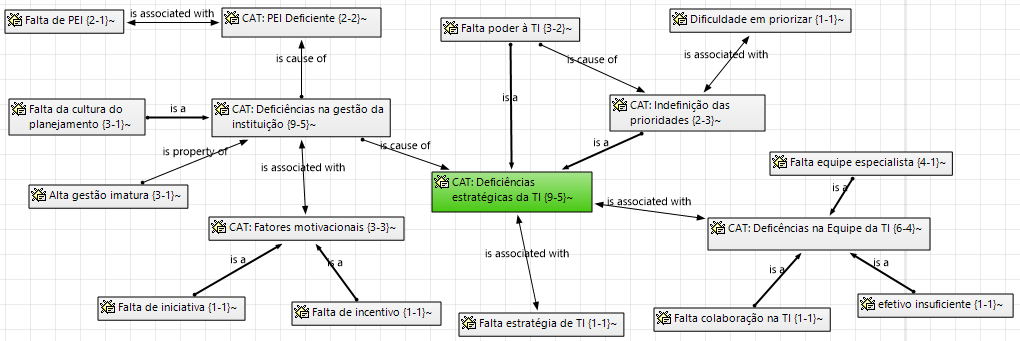
\includegraphics[width=15cm, frame]{figuras/sc_grupo1.PNG}
\caption{Esquema teórico do grupo 1 após a codificação seletiva.}
\label{figura:sc_grupo1}
\end{figure}

\begin{figure}[h!]
\centering % para centralizarmos a figura
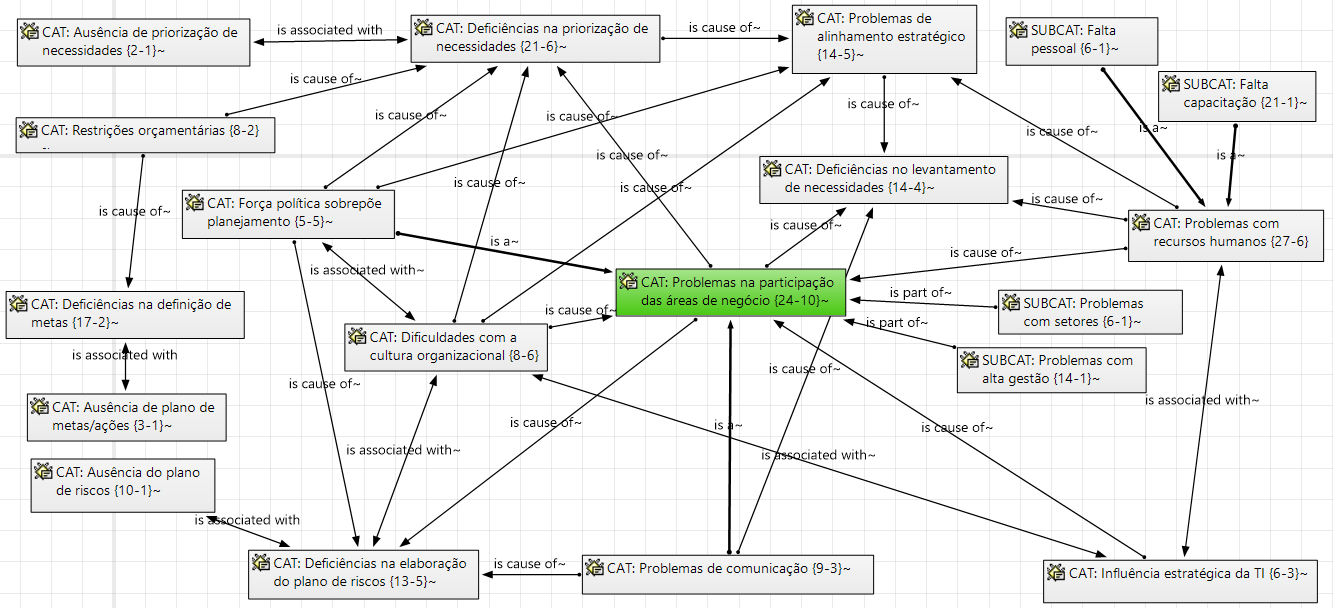
\includegraphics[width=15cm, frame]{figuras/sc_grupo2.PNG}
\caption{Esquema teórico do grupo 2 após a codificação seletiva.}
\label{figura:sc_grupo2}
\end{figure}



\section{Resultado: Teorias Fundamentadas nos Dados}
\label{secao:resultado_teorias}
Após a aplicação do método \textit{Grounded Theory}, foi possível visualizar as categorias centrais de cada grupo de dados e, através de seus relacionamentos e propriedades, traçar uma teoria para cada grupo pesquisado. Além dos esquemas teóricos, que representam graficamente a teoria central após as análises dos dados, uma teoria pode ser expressada através de um paradigma, contendo três elementos fundamentais: condição causal, fenômeno (categoria central) e consequência (questão da pesquisa) \cite{corbin:98}.

Uma teoria substantiva de qualidade deve estar isenta de arbitrariedade do pesquisador, sendo capaz de permitir seu livre escrutínio público por meio de auditorias que avaliem o pesquisador e o processo de pesquisa utilizado \cite{bandeira:03}.

Para o grupo 1, das instituições sem PDTI, a categoria central foi caracterizada como ``Deficiências estratégicas da TI''. Sua condição causal, ou seja, a razão que implica a categoria central foi caracterizada como ``nível baixo de maturidade em gestão''. A consequência disto é a ``ausência de planejamento de TI''. Diante disso, utilizando-se das propriedades das categorias envolvidas no paradigma causal, a teoria fundamentada nos dados sobre a ausência de um PDTI em uma instituição pode ser expressada da seguinte forma:

\textbf{Teoria para a ausência do PDTI nas instituições:} ``\textit{Uma instituição com baixo nível de maturidade em gestão não dá a devida importância à planos estratégicos e não reconhece a TI como parte estratégica da instituição. A área de TI, por sua vez, apresenta deficiências estratégicas como (a) baixo nível de influência da TI na instituição como um todo e (b) equipe inadequada em quantidade e em domínio de técnicas de planejamento; tais fatores impedem ou dificultam a elaboração do Plano Diretor de TI.}''

A Figura \ref{figura:paradigma1} apresenta um esquema teórico composto apenas dos códigos presentes na teoria para a ausência do PDTI nas instituições.

\begin{figure}[h!]
\centering % para centralizarmos a figura
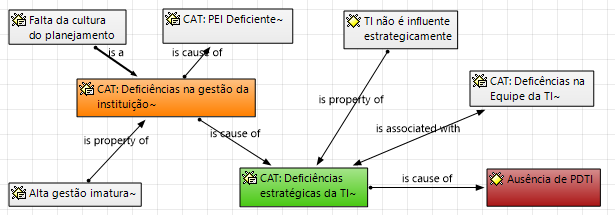
\includegraphics[width=13cm, frame]{figuras/paradigma1.PNG}
\caption{Esquema teórico da teoria 1.}
\label{figura:paradigma1}
\end{figure}


Para o grupo 2, das instituições com PDTI, a categoria central foi caracterizada como ``problemas na participação das áreas de negócio''. Sua condição causal, ou seja, a razão que implica a categoria central foi caracterizada como uma tríade de categorias: ``problemas de cultura organizacional'' + ``TI não reconhecida estrategicamente'' + ``problemas com recursos humanos''. A consequência disto são as ``dificuldades na elaboração do planejamento e PDTI com deficiências''. Diante disso, utilizando-se das propriedades das categorias envolvidas no paradigma causal, a teoria fundamentada nos dados sobre as dificuldades na elaboração de um PDTI em uma instituição pode ser expressada da seguinte forma:

\textbf{Teoria para as dificuldades na elaboração e deficiências do PDTI:} \textit{``Uma instituição que (i) possui membros que colocam interesses particulares e políticos acima dos interesses da instituição; (ii) não possui a percepção de que a TI é parte estratégica e (iii) não possuem recursos humanos devidamente capacitados para promover a cultura do planejamento, não apresenta o comprometimento e a participação satisfatória das áreas de negócio na composição do planejamento de TI. Tal participação das áreas de negócio é o fator que mais impacta nas dificuldades e deficiências apresentadas na elaboração do PDTI.''}

A Figura \ref{figura:paradigma2} apresenta um esquema teórico composto apenas dos códigos presentes na teoria para as dificuldades na elaboração e deficiências do PDTI.

\begin{figure}[h!]
\centering % para centralizarmos a figura
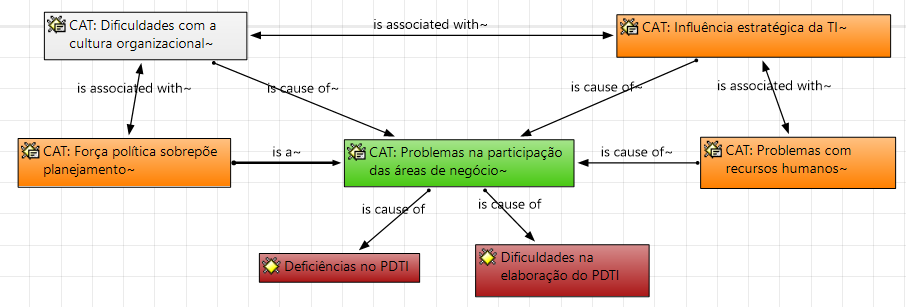
\includegraphics[width=13cm, frame]{figuras/paradigma2.PNG}
\caption{Esquema teórico da teoria 2.}
\label{figura:paradigma2}
\end{figure}

É possível verificar os passos da pesquisa que levaram às teorias apresentadas. O apêndice \ref{apendice:d_respostas_disserta} apresenta os dados na íntegra, conforme a respostas coletadas. O apêndice \ref{apendice:e_codigos} apresenta os códigos extraídos dos dados e os apêndices \ref{apendice:f_notas_ma} e \ref{apendice:h_notas_oc} apresentam as anotações feitas durante a fase de codificação aberta. Posteriormente, a fase de codificação axial, na qual descobre-se os relacionamentos entre os códigos, está descrita nas anotações presentes no apêndice \ref{apendice:i_notas_ac}.

\section{Avaliação dos Resultados}
\label{secao:avaliacao_resultados}
%Anexo B (contém as questões apenas)
O problema abordado neste trabalho exige que o pesquisador seja isento de hipóteses ou conclusões pré-concebidas, uma vez que a proposta desta pesquisa é permitir que os resultados sejam fielmente baseados nos dados coletados com os envolvidos no problema, garantindo que a conclusão seja o mais próxima possível da realidade. Na GT, a coleta dos dados, análise, formulação e a validação da teoria são reciprocamente relacionadas, em um processo indutivo de interpretação e em um processo de dedução e validação de proposições \cite{bandeira:03}.

Contudo, foi elaborado um questionário aplicado aos participantes da fase de coleta de dados. Tal questionário tem o objetivo de medir a aderência, através de escala de \textit{Likert}, da teoria resultante da pesquisa às dificuldades de planejamento de TI vivenciadas pelos respondentes.

Foram obtidas 32 avaliações de 23 instituições diferentes, de um total 37 instituições alvo. As avaliações foram divididas em dois grupos com perguntas específicas para cada grupo. O primeiro grupo é composto de membros de instituições que não possuem um PDTI, ao contrário do segundo grupo, composto por membros de instituições que já possuem um PDTI. O questionário aplicado nesta etapa da pesquisa é apresentado no \autoref{apendice:b_quest_avaliacao}.

Ao primeiro grupo foi apresentado a teoria sobre as razões que impedem a instituição de elaborar um PDTI. Em uma escala de zero a cinco, onde zero corresponde à ``discordo totalmente'' e cinco corresponde à ``concordo totalmente'', 100\% dos respondentes apontam que a teoria levantada é aderente à realidade. Deste total, 66,7\% concordam totalmente com a teoria. A Figura \ref{figura:grafico_ava_grupoSemPDTI} mostra a distribuição das respostas do primeiro grupo.


\begin{figure}[h]
\centering % para centralizarmos a figura
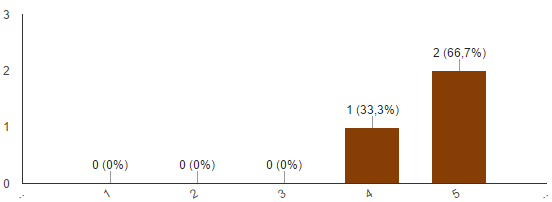
\includegraphics[width=10cm, frame]{figuras/grafico_ava_grupoSemPDTI.PNG}
\caption{Aderência à teoria sobre as razões da ausência de um PDTI}
\label{figura:grafico_ava_grupoSemPDTI}
\end{figure}

Ao segundo grupo foi apresentado a teoria sobre as dificuldades e deficiências encontradas em uma instituição ao elaborar seu PDTI. Em uma escala de zero a cinco, onde zero corresponde à ``discordo totalmente'' e cinco corresponde à ``concordo totalmente'', 79,3\% dos respondentes apontam que a teoria levantada é aderente à realidade. Enquanto 20,7\% optaram pela alternativa central da escala. A Figura \ref{figura:grafico_ava_grupoComPDTI} mostra a distribuição das respostas do segundo grupo.

\begin{figure}[h]
\centering % para centralizarmos a figura
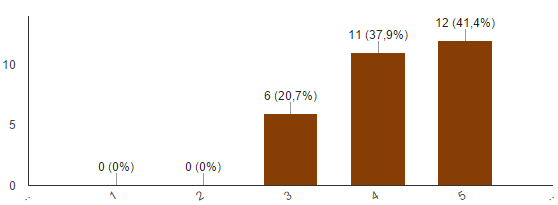
\includegraphics[width=10cm, frame]{figuras/grafico_ava_grupoComPDTI.PNG}
\caption{Aderência à teoria sobre as dificuldades na elaboração do PDTI}
\label{figura:grafico_ava_grupoComPDTI}
\end{figure}

Apesar de não ter atingido 100\% dos respondentes da coleta inicial de dados, os resultados apresentados no questionário de avaliação das teorias se mostraram, de forma geral, aderentes às teorias fundamentadas nos dados. Este resultado corrobora com os princípios da \textit{Grounded Theory}, que preza pelo empirismo no intuito de apresentar uma teoria próxima à realidade. Em outras palavras, os respondentes se viram representados na teoria.

\section{Considerações}
O processo de análise dos dados utilizando \textit{Grounded Theory} requer procedimentos metódicos e um profundo exercício de imparcialidade. Contudo, foi possível seguir os princípios da GT para atingir o objetivo da pesquisa.

Com o apoio da GT foi possível obter uma teoria fundamentada em dados que evidencia as principais causas das dificuldades de planejamento de TI nas instituições. Além disso, também através de uma teoria fundamentada nos dados, identificou-se as principais motivações que levam ao não cumprimento da determinação de se estabelecer o PDTI.

As teorias aqui apresentadas respondem à questão de pesquisa: ``apesar da obrigatoriedade e dos conhecidos benefícios, o planejamento de TI não é realizado satisfatoriamente nos órgãos públicos federais. A atividade de planejamento envolve aspectos técnicos e sociais, diante disso, pergunta-se: quais os fatores que dificultam o processo de elaboração do planejamento de TI e quais as relações entre tais fatores?''.

A descrição completa das teorias são as respostas da pergunta de pesquisa, contudo, de forma resumida pode-se responder a questão de pesquisa dividindo-a em duas partes:

1 - Quais os fatores que dificultam o processo de elaboração do planejamento de TI?\\
Resposta: Baseado na teoria fundamentada em dados, para as instituições que não conseguiram elaborar o PDTI, os fatores que dificultam este processo são (i) as deficiências na gestão da instituição, com baixo nível de maturidade em gestão estratégica; e principalmente (ii) as deficiências estratégicas da TI, ou seja, a área de TI não é reconhecida estrategicamente e possuem equipe inadequada em quantidade e competências para desenvolver atividades estratégicas.

Já nas instituições que possuem o PDTI, os fatores que dificultam o processo de elaboração passam por (i) influência política interna sobrepondo o planejamento; (ii) baixa influência estratégica da TI; (iii) problemas com recursos humanos em quantidade e capacidade para desenvolver as atividades de planejamento; e principalmente (iv) falta de comprometimento e participação satisfatória das áreas de negócio na elaboração do PDTI.

2 - Quais as relações entre os fatores?\\
Resposta: os fatores apresentam relação de causa e consequência, conforme esquematizado a seguir:
\\
\\
\textbf{Teoria 1:}\\
\textit{Condição causal:} Nível baixo de maturidade em gestão;\\
\textit{Fenômeno:} Deficiências estratégicas na TI;\\
\textit{Consequência:} Ausência de planejamento de TI.
\\
\\
\textbf{Teoria 2:}\\
\textit{Condição causal:} A tríade ``problemas de cultura organizacional'' + ``TI não reconhecida estrategicamente'' + ``problemas com recursos humanos'';\\
\textit{Fenômeno:} Problemas na participação das áreas de negócio;\\
\textit{Consequência:} Dificuldades na elaboração do planejamento e PDTI com deficiências.


Conclui-se que o método se mostrou eficaz em trazer à tona teorias que refletem os dados. Os resultados apresentados, teorias e avaliações, convergem para o cumprimento do objetivo desta pesquisa: elucidar o problema da elaboração do planejamento de TI nos órgãos federais identificando empiricamente os fatores e os relacionamentos que levam a este cenário. Diante disso, na seção seguinte são apresentadas sugestões de ações para minimizar os fatores que contribuem para as deficiências do planejamento de TI no setor público.
\chapter{Melhores práticas de planejamento de TI relacionadas ao problema do PDTI}
\label{capitulo:proposta_mp}

O foco desta pesquisa consiste em esclarecer as razões que culminam no problema de planejamento de TI das instituições públicas federais. A metodologia adotada nesta pesquisa permitiu expor os fatores que atrapalham as instituições a elaborarem o PDTI, na visão dos participantes desta atividade. Apesar destes elementos comporem o objetivo principal da presente pesquisa, propõe-se além disso, sugerir um conjunto de melhores práticas para atenuar os fatores que restringem a elaboração e a qualidade do PDTI.

As práticas propostas neste capítulo são inteiramente baseadas na tese de \citeonline{teixeira:10}. O autor propõe um modelo de maturidade para planejamento estratégico de SI/TI direcionado às organizações governamentais brasileiras (MMPE-SI/TI Gov) baseado em melhores práticas. O método \textit{Grounded Theory} também foi empregado nesta etapa da pesquisa com o intuito de prover rigor científico à seleção das melhores práticas que atingem diretamente os fatores causais presentes nas teorias resultantes.
%Diante do banco de melhores práticas proposto por \citeonline{teixeira:10}, foi feito o mapeamento daquelas que atingem diretamente os fatores presentes nas teorias resultantes desta pesquisa.


\section{Processos e Melhores Práticas de Planejamento de TI}
\label{secao:melhores_praticas}
``Melhores práticas (MP) são visões de organizações e profissionais globais que através da vivência no mercado conseguem perceber práticas, que se utilizadas em outras organizações podem melhorar seu desempenho da mesma forma'' \apud{kerzner:11,laudon:05}{teixeira:10}.

O modelo de maturidade MMPE-SI/TI (Gov) foi definido em conformidade com os principais modelos e normas nacionais e internacionais utilizados para definição e avaliação de processos, tais como ISO 12207/15504, COBIT, CMMI, MPS.BR, MMGP, OPM3, PMMM, leis e normativas do governo brasileiro. Sua estrutura é composta por um modelo de referência (MR), um método de avaliação (MA) e um banco de melhores práticas (BMP). 

O modelo MMPE-SI/TI (Gov) possui 5 níveis de maturidade, 6 níveis de capacidade, 16 processos e 124 melhores práticas para planejamento estratégico de SI/TI direcionadas às organizações governamentais brasileiras. A Tabela \ref{tabela:niveis_maturidade} apresenta os níveis de maturidade do modelo e seus processos.

\begin{table}[]
\centering
\begin{tabular}{|c|l|l|}
\hline
\rowcolor[HTML]{C0C0C0} 
\textbf{Nível} & \multicolumn{1}{c|}{\cellcolor[HTML]{C0C0C0}\textbf{Processos}}                                                                                                                                                                                & \multicolumn{1}{c|}{\cellcolor[HTML]{C0C0C0}\textbf{Áreas}}                                           \\ \hline
1 Inicial / ad hoc             & \begin{tabular}[c]{@{}l@{}}Promover Consciência Estratégica (PCE)\\ Assegurar Conformidade Governamental (ACG)\end{tabular}                                                                                                                    & \begin{tabular}[c]{@{}l@{}}Gestão\\ Organização\end{tabular}                                          \\ \hline
2 Gerenciado             & \begin{tabular}[c]{@{}l@{}}Gerenciar Recursos Humanos (GRH) \\ Educar e Treinar Pessoas (ETP) \\ Gerenciar Projetos (GEP) \\ Gerenciar Medição e Análise (GMA)\end{tabular}                                                                    & \begin{tabular}[c]{@{}l@{}}Pessoas\\ Pessoas\\ Gestão\\ Gestão\end{tabular}                           \\ \hline
3 Definido             & \begin{tabular}[c]{@{}l@{}}Definir o Processo Organizacional (DPO)\\ Gerenciar Aquisições e Terceirizações (GAT) \\ Gerenciar Infraestrutura de SI/TI (GIN) \\ Gerenciar Qualidade (GQA) \\ Fomentar Gestão do Conhecimento (FGC)\end{tabular} & \begin{tabular}[c]{@{}l@{}}Organização\\ Organização\\ Tecnologia\\ Gestão\\ Organização\end{tabular} \\ \hline
4 Medido             & \begin{tabular}[c]{@{}l@{}}Avaliar o Processo Organizacional (APO) \\ Gerenciar Riscos (GRI) \\ Gerenciar Integração com o Cidadão (GIC)\end{tabular}                                                                                          & \begin{tabular}[c]{@{}l@{}}Organização\\ Gestão\\ Pessoas\end{tabular}                                \\ \hline
5 Otimizado             & \begin{tabular}[c]{@{}l@{}}Melhorar o Processo Organizacional (MPO)\\  Otimizar a Gestão Organizacional (OGO)\end{tabular}                                                                                                                     & \begin{tabular}[c]{@{}l@{}}Organização\\ Gestão\end{tabular}                                          \\ \hline
\end{tabular}
\caption{Níveis de Maturidade do MMPE-SI/TI (Gov) e seus Processos, extraído de \cite{teixeira:10}}
\label{tabela:niveis_maturidade}
\end{table}

Cada processo contém um conjunto de melhores práticas (MP) e resultados esperados (RE). A seleção das MP aderentes aos cenários levantados nesta pesquisa - em relação ao problema do planejamento de TI - tem o intuito de sugerir um caminho para atenuar os efeitos das condições causais e dos fenômenos centrais das teorias que emergiram dos dados. O procedimento realizado para selecionar as MP relacionadas com as duas teorias fundamentadas nos dados desta pesquisa é descrito na seção seguinte.

%Ao traçar relações entre MP, condições causais e os fenômenos centrais, busca-se oferecer meios para reduzir as consequências (problemas na elaboração do planejamento de TI). Este objetivo foi possível investigando possíveis relações entre os processos do MMPE-SI/TI e os elementos das teorias que emergiram dos dados nesta pesquisa. Este procedimento é descrito na seção seguinte. 
%Diante do exposto, o objetivo secundário desta pesquisa se propõe a realizar uma seleção das melhores práticas de planejamento estratégico de SI/TI direcionadas aos fatores que restringem o planejamento de TI nas instituições pesquisadas.
\section{Seleção das Melhores Práticas}

Para manter a coerência de fundamentação dos resultados desta pesquisa, optou-se por utilizar o mesmo método usado para gerar as teorias também na etapa de seleção das melhores práticas. A \textit{Grounded Theory} é aplicada neste contexto com o intuito de manter a fidelidade empírica que a teoria fundamentada nos dados carrega ao relacioná-la com processos e melhores práticas de planejamento de TI. Desta forma, a arbitrariedade do pesquisador ao selecionar as MP é reduzida e o grau de fundamentação nos dados é maximizado.

Buscou-se por relacionamentos entre elementos das teorias apresentadas nesta pesquisa e processos do MMPE-SI/TI (Gov) que, por sua vez, carregam seus respectivos conjuntos de MP. Assim, o esforço nesta etapa da pesquisa concentra-se em descobrir as relações semânticas entre as teorias fundamentadas nos dados e os processos de planejamento de TI do modelo de maturidade estudado. As melhores práticas já foram relacionadas aos processos no trabalho de \citeonline{teixeira:10} e serão apontadas como consequência do relacionamento com os processos. A Figura \ref{figura:esquemaconjuntos} representa graficamente esta ideia, onde as setas pontilhadas são os relacionamentos que se deseja descobrir.

\begin{figure}[h!]
\centering % para centralizarmos a figura
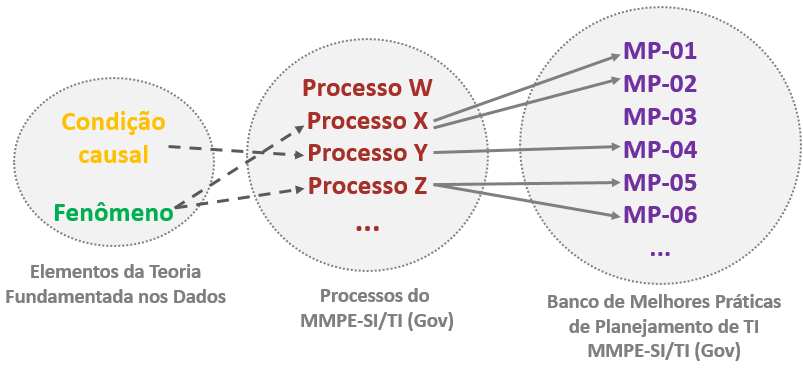
\includegraphics[width=13cm]{figuras/conjuntos_relacionamentos.PNG}
\caption{Esquema de relacionamento entre elementos da teoria e processos de planejamento.}
\label{figura:esquemaconjuntos}
\end{figure}

Para focar a busca por processos diretamente relacionados aos elementos centrais das teorias, as mesmas foram reescritas na forma de paradigma, conforme descreve \citeonline{corbin:98}. Abaixo, cada uma das teorias com seus respectivos elementos organizados de acordo com o paradigma causal:
\\
\\
\textbf{Teoria 1:}\\
\textit{Condição causal:} Nível baixo de maturidade em gestão;\\
\textit{Fenômeno:} Deficiências estratégicas na TI;\\
\textit{Consequência:} Ausência de planejamento de TI.
\\
\\
\textbf{Teoria 2:}\\
\textit{Condição causal:} A tríade ``problemas de cultura organizacional'' + ``TI não reconhecida estrategicamente'' + ``problemas com recursos humanos'';\\
\textit{Fenômeno:} Problemas na participação das áreas de negócio;\\
\textit{Consequência:} Dificuldades na elaboração do planejamento e PDTI com deficiências.

De posse dos elementos de cada teoria e dos processos do modelo MMPE-SI/TI (Gov), aplicou-se a \textit{Grounded Theory} para traçar as relações entre estes dois grupos de dados. Como não há nesta fase o objetivo de gerar uma nova teoria ou eleger uma categoria central, aplicou-se apenas as etapas de codificação aberta e axial.

\subsection{Codificação Aberta}

Diferentemente da primeira etapa desta pesquisa, onde foi necessário identificar os códigos nos dados coletados através dos questionários, nesta segunda aplicação do método GT aproveitou-se os códigos (categorias) da primeira etapa. Porém, para relacionar as categorias da teoria existente aos processos do MMPE-SI/TI, se faz necessário codificá-los.

Cada processo do MMPE-SI/TI foi codificado como uma categoria, rotulada com o mesmo nome do processo. O a descrição da categoria é o próprio propósito do processo descrito por \citeonline{teixeira:10}. Os resultados esperados de cada processo definem os mesmos, ou seja, o conjunto de RE de cada processo podem ser considerados como propriedades das categorias. Abaixo é apresentado um exemplo da codificação aberta de um dos processos. A Tabela \ref{tabela:mmpe_to_gt} mostra os dados extraídos do MMPE-SI/TI e os itens correspondentes na codificação aberta.

%PAREI AQUI: fazer tabela
% Please add the following required packages to your document preamble:
% \usepackage[table,xcdraw]{xcolor}
% If you use beamer only pass "xcolor=table" option, i.e. \documentclass[xcolor=table]{beamer}
\begin{table}[]
\centering
\resizebox{\textwidth}{!}{%
\begin{tabular}{|l|l|}
\hline
\rowcolor[HTML]{C0C0C0} 
\multicolumn{1}{|c|}{\cellcolor[HTML]{C0C0C0}\textbf{MMPE-SI/TI (Gov)}}                                                                                                                                                                                                                                                                                       & \multicolumn{1}{c|}{\cellcolor[HTML]{C0C0C0}\textbf{Grounded Theory}}                                                                                                                                                                                                                                                                            \\ \hline
\textbf{Processo:} Educar e Treinar Pessoas (ETP)                                                                                                                                                                                                                                                                                                                      & \textbf{Categoria:} CAT Educar e Treinar Pessoas                                                                                                                                                                                                                                                                                                          \\ \hline
\begin{tabular}[c]{@{}l@{}}\textbf{Propósito:} Entender claramente as necessidades\\ das pessoas (diretores, gerentes e usuários) em \\ termos de educação e treinamento em SI/TI e \\ executar uma estratégia eficaz de treinamento \\ e medição dos resultados.\end{tabular}                                                                                         & \begin{tabular}[c]{@{}l@{}}\textbf{Conceito:} Entender claramente as necessidades\\ das pessoas (diretores, gerentes e usuários) em \\ termos de educação e treinamento em SI/TI e \\ executar uma estratégia eficaz de treinamento\\ e medição dos resultados.\end{tabular}                                                                              \\ \hline
\begin{tabular}[c]{@{}l@{}}\textbf{Resultados Esperados (RE):}\\ ETP-RE-01: Treinamentos para tratar das \\ necessidades da organização são desenvolvidos\\ ou adquiridos;\\ \\ ETP-RE-02: Treinamentos para garantir que \\ todos os indivíduos têm habilidades necessárias \\ para executar as suas tarefas são realizados, \\ monitorados e avaliados.\end{tabular} & \begin{tabular}[c]{@{}l@{}}\textbf{Propriedades:}\\ ETP-RE-01: Treinamentos para tratar das \\ necessidades da organização são desenvolvidos\\ ou adquiridos;\\ \\ ETP-RE-02: Treinamentos para garantir que \\ todos os indivíduos têm habilidades necessárias \\ para executar as suas tarefas são realizados, \\ monitorados e avaliados.\end{tabular} \\ \hline
\end{tabular}%
}
\caption{Exemplo de categoria codificada a partir de um processo.}
\label{tabela:mmpe_to_gt}
\end{table}

O procedimento de codificar os processos em categorias foi realizado com os 16 processos do modelo de maturidade, portanto acrescentando 16 novas categorias ao conjunto de códigos de cada uma das duas teorias fundamentadas nos dados. O passo seguinte é pesquisar por relacionamentos entre as novas categorias e as categorias de cada teoria central, este procedimento é realizado na codificação axial.

\subsection{Codificação Axial}
A codificação axial tem por objetivo descobrir possíveis relações entre categorias. O procedimento para realizar esta codificação, assim como realizado para descobrir as teorias, consiste em colocar cada categoria como eixo e buscar relações semânticas com outras categorias \cite{glaser:68, corbin:98}.

Os conectores usados na codificação axial para descobrir as teorias foram: \textit{is a}, \textit{is cause of}, \textit{is part of} e \textit{is associated with}. Contudo, nesta etapa da pesquisa, estes conectores não são compatíveis com a semântica que a análise dos dados demonstrou. As categorias extraídas do modelo de maturidade apresentam um sentido de efeitos de uma solução, ao contrário das categorias das teorias que apresentam sentido de causas de problemas. 

Neste cenário, \citeonline{corbin:98} apresenta o tipo de relacionamento denominado ``condição interveniente''. A condição interveniente representa relacionamentos onde o código origem representa um conceito que pode reduzir ou alterar o impacto do código destino no fenômeno. Desta forma, é possível representar relações entre códigos que possuem sentido oposto um ao outro. Com isto, foi introduzido o conector \textit{contradicts} para representar as condições intervenientes.

A descoberta dos relacionamentos entre as teorias sobre os problemas de planejamento de TI e os processos do modelo de maturidade foi facilitada observando os resultados esperados de cada processo. Observa-se que os RE são opostos às propriedades das categorias da teoria. As análises apontam para a seguinte linha de pensamento: a instituição que apresenta estes fatores causais (do problema) não apresenta os resultados esperados deste processo. 

Para a teoria 1, das instituições que não possuem PDTI, a codificação axial permitiu trazer à tona 4 processos que impactam diretamente nas causas do problema: Promover Consciência Estratégica (PCE); Gerenciar Recursos Humanos (GRH); Educar e Treinar Pessoas (ETP); Gerenciar Projetos (GEP). A Figura \ref{figura:teoria_processos_grupo1} apresenta o esquema teórico dos elementos da teoria 1 e as categorias de processos que apresentaram pelo menos um relacionamento com a teoria.

\begin{figure}[h!]
\centering % para centralizarmos a figura
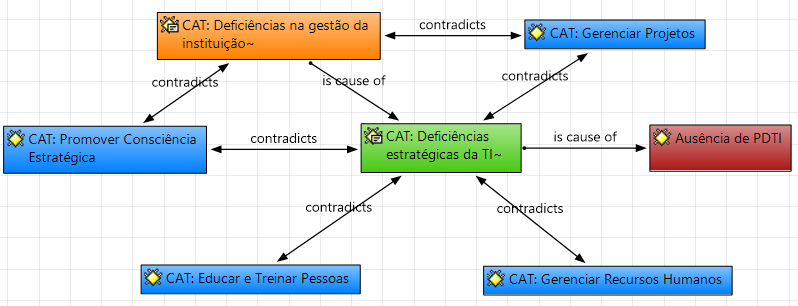
\includegraphics[width=15cm]{figuras/teoria_processos_grupo1.PNG}
\caption{Esquema teórico: Teoria 1 - Processos MMPE-SI/TI}
\label{figura:teoria_processos_grupo1}
\end{figure}

Para a teoria 2, das instituições que possuem PDTI, a codificação axial permitiu trazer à tona 5 processos que impactam diretamente nas causas do problema: Promover Consciência Estratégica (PCE); Gerenciar Recursos Humanos (GRH); Educar e Treinar Pessoas (ETP); Gerenciar Projetos (GEP); Otimizar a Gestão Organizacional (OGO). A Figura \ref{figura:teoria_processos_grupo2} apresenta o esquema teórico dos elementos da teoria 2 e as categorias de processos que apresentaram pelo menos um relacionamento com a teoria.

\begin{figure}[h!]
\centering % para centralizarmos a figura
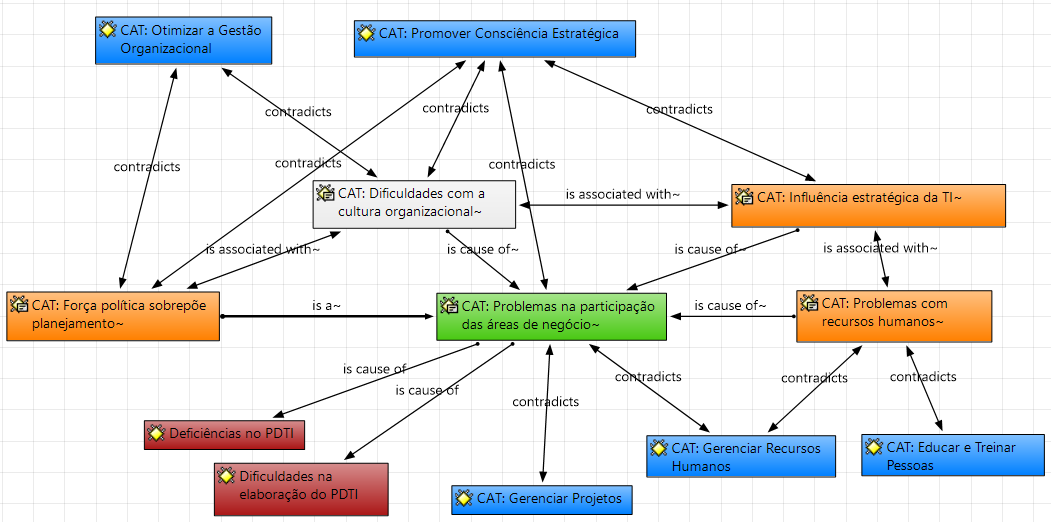
\includegraphics[width=15cm]{figuras/teoria_processos_grupo2.PNG}
\caption{Esquema teórico: Teoria 2 - Processos MMPE-SI/TI}
\label{figura:teoria_processos_grupo2}
\end{figure}

As análises foram registradas em notas de codificação axial e permitem compreender a relação semântica entre os códigos. De forma geral, foi observado que as relações eram descobertas analisando como o propósito e os resultados esperados do processo contrastavam com as categorias da teoria. Todas as notas de codificação axial desta etapa da pesquisa estão listadas no apêndice \autoref{apendice:j_notas_ac}.

É importante observar que o fenômeno central de ambas as teorias foi o elemento causal que concentrou mais relacionamentos com as categorias que representam os processos de planejamento de TI. Este efeito corrobora a conclusão de que as ``deficiências estratégicas da TI'' representam a principal causa da falta de PDTI (Teoria 1); e que os ``problemas na participação das áreas de negócio no planejamento de TI'' representam a principal causa das dificuldades de elaboração e deficiências no planejamento de TI das instituições que possuem PDTI.

\subsection{Melhores Práticas para Minimizar o Problema do PDTI}
\label{secao:mp_finais}

Ao aplicar as técnicas da \textit{Grounded Theory} foi possível vincular a teoria fundamentada nos dados que explica as causas dos problemas do PDTI nas instituições pesquisadas com os processos de planejamento de TI do MMPE-SI/TI (Gov). A Tabela \ref{tabela:processo_teoria} apresenta os processos de planejamento envolvidos diretamente com cada elemento causal das teorias.

\begin{table}[h!]
\centering
\resizebox{\textwidth}{!}{%
\begin{tabular}{c|l|l|}
\cline{2-3}
\textbf{}                                                                                                 & \multicolumn{1}{c|}{\cellcolor[HTML]{C0C0C0}\textbf{Elemento causal}}                                       & \multicolumn{1}{c|}{\cellcolor[HTML]{C0C0C0}\textbf{Processos envolvidos}}                                                                                                    \\ \hline
\multicolumn{1}{|c|}{\cellcolor[HTML]{C0C0C0}\textbf{\begin{tabular}[c]{@{}c@{}}Teoria\\ 1\end{tabular}}} & Deficiências na gestão da instituição                                                                       & \begin{tabular}[c]{@{}l@{}}PCE - Promover Consciência Estratégica\\ GEP - Gerenciar Projetos\end{tabular}                                                                     \\ \cline{2-3} 
\multicolumn{1}{|c|}{\cellcolor[HTML]{C0C0C0}\textbf{}}                                                   & Deficiências estratégicas na TI                                                                             & \begin{tabular}[c]{@{}l@{}}PCE - Promover Consciência Estratégica\\ GEP - Gerenciar Projetos\\ GRH - Gerenciar Recursos Humanos\\ ETP - Educar e Treinar Pessoas\end{tabular} \\ \hline
\multicolumn{1}{|c|}{\cellcolor[HTML]{C0C0C0}\textbf{\begin{tabular}[c]{@{}c@{}}Teoria\\ 2\end{tabular}}} & Problemas na cultura organizacional                                                                         & \begin{tabular}[c]{@{}l@{}}PCE - Promover Consciência Estratégica\\ OGO - Otimizar a Gestão Organizacional\end{tabular}                                                       \\ \cline{2-3} 
\multicolumn{1}{|c|}{\cellcolor[HTML]{C0C0C0}\textbf{}}                                                   & TI não reconhecida estrategicamente                                                                         & PCE - Promover Consciência Estratégica                                                                                                                                        \\ \cline{2-3} 
\multicolumn{1}{|c|}{\cellcolor[HTML]{C0C0C0}\textbf{}}                                                   & Problemas com recursos humanos                                                                              & \begin{tabular}[c]{@{}l@{}}GRH - Gerenciar Recursos Humanos\\ ETP - Educar e Treinar Pessoas\end{tabular}                                                                     \\ \cline{2-3} 
\multicolumn{1}{|c|}{\cellcolor[HTML]{C0C0C0}\textbf{}}                                                   & \begin{tabular}[c]{@{}l@{}}Problemas na participação das áreas\\ negócio no planejamento de TI\end{tabular} & \begin{tabular}[c]{@{}l@{}}PCE - Promover Consciência Estratégica\\ GRH - Gerenciar Recursos Humanos\\ GEP - Gerenciar Projetos\end{tabular}                                  \\ \hline
\end{tabular}%
}
\caption{Processos relacionados às teorias fundamentadas nos dados.}
\label{tabela:processo_teoria}
\end{table}

O propósito de cada um destes processos é descrito por \citeonline{teixeira:10} a seguir:

%Diante disso, foram mapeados um total de cinco processos que, se executados, podem contribuir para a melhoria da situação do planejamento de TI nas instituições públicas pesquisadas. O propósito de cada um destes processos é descrito por \citeonline{teixeira:10} a seguir:

\textbf{Promover Consciência Estratégica (PCE):} Habilitar a organização, através da alta administração, a entender as questões estratégicas de SI/TI, tais como os papéis de SI/TI, as capacidades e os conhecimentos tecnológicos, além de certificar-se de que há um entendimento comum entre o negócio e SI/TI, principalmente quanto ao potencial de contribuição que SI/TI proporciona para a estratégia do negócio.

%\textbf{Assegurar Conformidade Governamental (ACG):} Assegurar que a organização esteja em conformidade com os requisitos contratuais e legais (leis, decretos, instruções normativas, entre outras regulamentações) estabelecidas pelo governo brasileiro.

\textbf{Gerenciar Recursos Humanos (GRH):} Gerenciar os recursos humanos da organização e manter suas competências de acordo com as necessidades do negócio, além de motivar o pessoal de SI/TI através de planos de carreira, atribuição de funções coerentes com suas habilidades, definição de um processo de revisão do desempenho profissional, criação de descrições dos cargos, trabalho em grupo e minimização da dependência de indivíduos-chave.

\textbf{Educar e Treinar Pessoas (ETP):} Entender claramente as necessidades das pessoas (diretores, gerentes e usuários) em termos de educação e treinamento em SI/TI e executar uma estratégia eficaz de treinamento e medição dos resultados.

\textbf{Gerenciar Projetos (GEP):} Identificar, estabelecer, coordenar e monitorar as atividades, tarefas e recursos necessários para um projeto (planejamento de TI), com o objetivo de produzir um produto e/ou serviço, no contexto das necessidades do projeto e de suas restrições.

\textbf{Otimizar a Gestão Organizacional (OGO):} Otimizar e aperfeiçoar a gestão estratégica de SI/TI e as melhores práticas para planejamento estratégico de SI/TI da organização, buscando aumentar continuamente o alinhamento e a consistência com os objetivos estratégicos de negócio.


De acordo com o modelo de maturidade proposto por \citeonline{teixeira:10}, cada processo possui um conjunto de melhores práticas (MP). A seguir são apresentadas as 48 MP, propostas no MMPE-SI/TI (Gov), dos processos mapeados anteriormente.

\textbf{Melhores práticas do processo PCE: }
\\PCE-MP-01: Desenvolver uma Visão Estratégica; 
\\PCE-MP-02: Definir a Estrutura do Processo;
\\PCE-MP-03: Definir uma Estratégia;
\\PCE-MP-04: Consolidar o Compromisso com a Alta Administração;
\\PCE-MP-05: Comunicar a Visão e os Objetivos;
\\PCE-MP-06: Garantir o Compartilhamento de uma Visão Comum;
\\PCE-MP-07: Habilitar a Participação Ativa dos Stakeholders;
\\PCE-MP-08: Estabelecer um Comitê Estratégico de SI/TI (comitê de TI);
\\PCE-MP-09: Estabelecer um Plano Estratégico de SI/TI (ou PDTI).

\textbf{Melhores práticas do processo GRH: }
\\GRH-MP-01: Identificar Habilidades e Competências;
\\GRH-MP-02: Definir Critérios de Avaliação;
\\GRH-MP-03: Estabelecer um Programa de Recrutamento;
\\GRH-MP-04: Desenvolver Habilidades e Competências;
\\GRH-MP-05: Definir a Organização das Equipes;
\\GRH-MP-06: Conscientizar os Indivíduos sobre o Trabalho em Equipe;
\\GRH-MP-07: Manter as Interações das Equipes;
\\GRH-MP-08: Avaliar o Desempenho das Equipes;
\\GRH-MP-09: Fornecer Feedback sobre o Desempenho;
\\GRH-MP-10: Manter Registros de Pessoal;
\\GRH-MP-11: Minimizar a Dependência de Indivíduos-Chave;
\\GRH-MP-12: Organizar a Mudança e Desligamento do Cargo.

\textbf{Melhores práticas do processo ETP: }
\\ETP-MP-01: Desenvolver uma Estratégia de Treinamento;
\\ETP-MP-02: Identificar as Necessidades de Treinamento;
\\ETP-MP-03: Desenvolver ou Adquirir Treinamento;
\\ETP-MP-04: Preparar para Executar o Treinamento;
\\ETP-MP-05: Realizar o Treinamento do Pessoal;
\\ETP-MP-06: Manter os Registros de Treinamento;
\\ETP-MP-07: Avaliar a Eficácia do Treinamento.

\textbf{Melhores práticas do processo GEP: }
\\GEP-MP-01: Definir o Escopo do Projeto;
\\GEP-MP-02: Definir o Ciclo de Vida do Projeto;
\\GEP-MP-03: Avaliar a Viabilidade do Projeto;
\\GEP-MP-04: Determinar e Manter Estimativas para o Projeto;
\\GEP-MP-05: Definir as Atividades do Projeto;
\\GEP-MP-06: Definir as Necessidades de Experiências, Conhecimentos e Habilidades;
\\GEP-MP-07: Definir o Cronograma do Projeto;
\\GEP-MP-08: Identificar e Monitorar as Interfaces do Projeto;
\\GEP-MP-09: Atribuir Responsabilidades e Gerar Comprometimento;
\\GEP-MP-10: Estabelecer o Plano de Projeto;
\\GEP-MP-11: Implementar o Plano de Projeto;
\\GEP-MP-12: Monitorar o Projeto;
\\GEP-MP-13: Revisar o Progresso do Projeto;
\\GEP-MP-14: Corrigir os Desvios;
\\GEP-MP-15: Registrar Lições Aprendidas.

\textbf{Melhores práticas do processo OGO: }
\\OGO-MP-01: Priorizar Investimentos em Gestão Estratégica de SI/TI;
\\OGO-MP-02: Identificar Melhorias para Gestão Estratégica de SI/TI;
\\OGO-MP-03: Avaliar a Eficácia das Melhores Práticas;
\\OGO-MP-04: Aperfeiçoar as Melhores Práticas;
\\OGO-MP-05: Otimizar a Utilização das Melhores Práticas.


%
%Propõe-se, então, às instituições que enfrentam os problemas levantados nesta pesquisa que implementem os processos correspondentes ao cenário em que se encaixa. Em um primeiro cenário (grupo 1), instituições que ainda não possuem um PDTI e deseja minimizar os fatores que as impedem de elaborar o plano. O segundo cenário (grupo 2) engloba instituições que possuem um PDTI, mas que desejam minimizar as dificuldades na elaboração do plano. A Figura \ref{figura:processos_grupos} apresenta as camadas de processos que cada grupo precisa implementar. A ordem sugerida para implantação dos processos é da base para o topo da pirâmide.
%
%\begin{figure}[h!]
%\centering % para centralizarmos a figura
%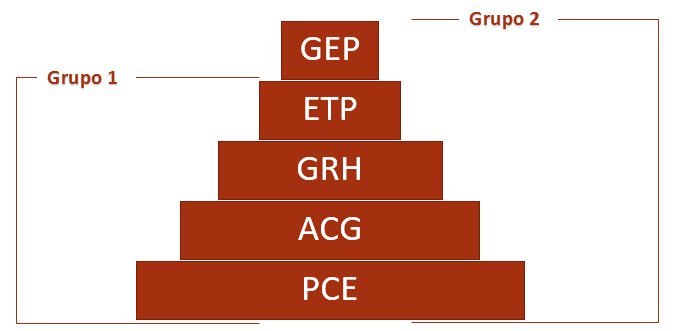
\includegraphics[width=8cm]{figuras/processos_grupos.PNG}
%\caption{Processos a serem implantados em cada cenário.}
%\label{figura:processos_grupos}
%\end{figure}

Tomando cada processo como eixo, as Tabelas \ref{tabela:acoes_1}, \ref{tabela:acoes_3}, \ref{tabela:acoes_4},  \ref{tabela:acoes_5} e \ref{tabela:acoes_2} apresentam as melhores de cada processo e seus respectivos resultados esperados.


\begin{table}[H]
\centering
\begin{tabular}{|l|l|}
\hline
\rowcolor[HTML]{C0C0C0} 
\multicolumn{1}{|c|}{\cellcolor[HTML]{C0C0C0}\textbf{MP}}                      & \multicolumn{1}{c|}{\cellcolor[HTML]{C0C0C0}\textbf{Resultados esperados}}                                                                                                                                   \\ \hline
\begin{tabular}[c]{@{}l@{}}PCE-MP-01\\ PCE-MP-09\end{tabular}                         & Os objetivos de negócio e de TI são identificados.                                                                                                                                                           \\ \hline
\begin{tabular}[c]{@{}l@{}}PCE-MP-02\\ PCE-MP-09\end{tabular}                         & \begin{tabular}[c]{@{}l@{}}A estrutura do processo que inclui um conjunto de \\ processos necessários para alcançar os objetivos de \\ negócio e de TI é identificado e definido.\end{tabular}               \\ \hline
\begin{tabular}[c]{@{}l@{}}PCE-MP-03\\ PCE-MP-04\\ PCE-MP-09\end{tabular}             & \begin{tabular}[c]{@{}l@{}}A estratégia para definição, implementação e melhoria\\ de processos é definida e o suporte para habilitar a \\ estratégia é fornecido.\end{tabular}                              \\ \hline
\begin{tabular}[c]{@{}l@{}}PCE-MP-05\\ PCE-MP-06\\ PCE-MP-07\\ PCE-MP-09\end{tabular} & \begin{tabular}[c]{@{}l@{}}A missão, visão, valores, cultura, objetivos e metas tanto \\ da organização quanto de TI são conhecidos e \\ compartilhados com todos os indivíduos da organização.\end{tabular} \\ \hline
\begin{tabular}[c]{@{}l@{}}PCE-MP-07\\ PCE-MP-09\end{tabular}                         & \begin{tabular}[c]{@{}l@{}}Cada indivíduo na organização compreende seu papel na \\ consecução dos objetivos de negócio e de TI e é \\ capaz de desempenhá-lo.\end{tabular}                                  \\ \hline
\begin{tabular}[c]{@{}l@{}}PCE-MP-08\\ PCE-MP-09\end{tabular}                         & Um comitê TI é estabelecido.                                                                                                                                                                                 \\ \hline
\end{tabular}
\caption{Melhores Práticas e Resultados Esperados do processo PCE, baseado em \cite{teixeira:10}.}
\label{tabela:acoes_1}
\end{table}

\begin{table}[H]
\centering
\begin{tabular}{|l|l|}
\hline
\rowcolor[HTML]{C0C0C0} 
\multicolumn{1}{|c|}{\cellcolor[HTML]{C0C0C0}\textbf{MP}}                                         & \multicolumn{1}{c|}{\cellcolor[HTML]{C0C0C0}\textbf{Resultados esperados}}                                                                                                    \\ \hline
\begin{tabular}[c]{@{}l@{}}GRH-MP-01\\ GRH-MP-02\\ GRH-MP-03\\ GRH-MP-04\\ GRH-MP-08\end{tabular} & \begin{tabular}[c]{@{}l@{}}As habilidades e competências necessárias para o \\ pessoal de TI são identificadas.\end{tabular}                                                  \\ \hline
\begin{tabular}[c]{@{}l@{}}GRH-MP-05\\ GRH-MP-06\\ GRH-MP-07\end{tabular}                         & \begin{tabular}[c]{@{}l@{}}A efetiva interação entre indivíduos e equipes é \\ suportada e os recursos humanos necessários\\  para a organização são fornecidos.\end{tabular} \\ \hline
GRH-MP-4                                                                                          & \begin{tabular}[c]{@{}l@{}}As habilidades necessárias para partilhar informações\\  e coordenar as atividades da equipe são desenvolvidas\\ com eficiência.\end{tabular}      \\ \hline
\begin{tabular}[c]{@{}l@{}}GRH-MP-02\\ GRH-MP-08\\ GRH-MP-09\\ GRH-MP-10\end{tabular}             & \begin{tabular}[c]{@{}l@{}}Critérios objetivos para avaliar, monitorar e melhorar\\ o desempenho do pessoal de SI/TI são estabelecidos.\end{tabular}                          \\ \hline
\begin{tabular}[c]{@{}l@{}}GRH-MP-11\\ GRH-MP-12\end{tabular}                                     & \begin{tabular}[c]{@{}l@{}}As dependências excessivas de indivíduos-chave são\\ minimizadas.\end{tabular}                                                                     \\ \hline
\end{tabular}
\caption{Melhores Práticas e Resultados Esperados do processo GRH, baseado em \cite{teixeira:10}.}
\label{tabela:acoes_3}
\end{table}


\begin{table}[H]
\centering
\begin{tabular}{|l|l|}
\hline
\rowcolor[HTML]{C0C0C0} 
\multicolumn{1}{|c|}{\cellcolor[HTML]{C0C0C0}\textbf{MP}}                             & \multicolumn{1}{c|}{\cellcolor[HTML]{C0C0C0}\textbf{Resultados esperados}}                                                                                                                         \\ \hline
\begin{tabular}[c]{@{}l@{}}ETP-MP-01\\ ETP-MP-02\\ ETP-MP-03\\ ETP-MP-04\end{tabular} & \begin{tabular}[c]{@{}l@{}}Treinamentos para tratar das necessidades da \\ organização são desenvolvidos ou adquiridos.\end{tabular}                                                               \\ \hline
\begin{tabular}[c]{@{}l@{}}ETP-MP-05\\ ETP-MP-06\\ ETP-MP-07\end{tabular}             & \begin{tabular}[c]{@{}l@{}}Treinamentos para garantir que todos os indivíduos \\ têm habilidades necessárias para executar as suas \\ tarefas são realizados, monitorados e avaliados\end{tabular} \\ \hline
\end{tabular}
\caption{Melhores Práticas e Resultados Esperados do processo ETP, baseado em \cite{teixeira:10}.}
\label{tabela:acoes_4}
\end{table}


\begin{table}[H]
\centering
\begin{tabular}{|l|l|}
\hline
\rowcolor[HTML]{C0C0C0} 
\multicolumn{1}{|c|}{\cellcolor[HTML]{C0C0C0}\textbf{MP}}                             & \multicolumn{1}{c|}{\cellcolor[HTML]{C0C0C0}\textbf{Resultados esperados}}                                                                                                      \\ \hline
\begin{tabular}[c]{@{}l@{}}GEP-MP-01\\ GEP-MP-02\end{tabular}                         & O escopo do projeto é definido.                                                                                                                                                 \\ \hline
\begin{tabular}[c]{@{}l@{}}GEP-MP-03\\ GEP-MP-04\end{tabular}                         & \begin{tabular}[c]{@{}l@{}}A viabilidade da realização do projeto diante \\ dos recursos disponíveis e das restrições\\ identificadas é avaliada.\end{tabular}                  \\ \hline
\begin{tabular}[c]{@{}l@{}}GEP-MP-05\\ GEP-MP-06\end{tabular}                         & \begin{tabular}[c]{@{}l@{}}As tarefas e os recursos necessários para \\ concluir o projeto são dimensionados e estimados.\end{tabular}                                          \\ \hline
GEP-MP-08                                                                             & \begin{tabular}[c]{@{}l@{}}Interfaces entre os elementos do projeto com\\ outros projetos são identificados e controlados.\end{tabular}                                         \\ \hline
\begin{tabular}[c]{@{}l@{}}GEP-MP-07\\ GEP-MP-09\\ GEP-MP-10\\ GEP-MP-11\end{tabular} & \begin{tabular}[c]{@{}l@{}}Os planos para a execução do projeto são \\ desenvolvidos e implementados.\end{tabular}                                                              \\ \hline
\begin{tabular}[c]{@{}l@{}}GEP-MP-11\\ GEP-MP-12\\ GEP-MP-13\end{tabular}             & O progresso do projeto é monitorado e relatado.                                                                                                                                 \\ \hline
\begin{tabular}[c]{@{}l@{}}GEP-MP-14\\ GEP-MP-15\end{tabular}                         & \begin{tabular}[c]{@{}l@{}}Medidas para corrigir os desvios do plano e para\\  prevenir a recorrência dos problemas identificados\\  no projeto são estabelecidas.\end{tabular} \\ \hline
\end{tabular}
\caption{Melhores Práticas e Resultados Esperados do processo GEP, baseado em \cite{teixeira:10}.}
\label{tabela:acoes_5}
\end{table}

\begin{table}[H]
\centering
\begin{tabular}{|l|l|}
\hline
\rowcolor[HTML]{C0C0C0} 
\multicolumn{1}{|c|}{\cellcolor[HTML]{C0C0C0}\textbf{MP}}                 & \multicolumn{1}{c|}{\cellcolor[HTML]{C0C0C0}\textbf{Resultados esperados}}                                                                                                          \\ \hline
OGO-MP-01                                                                 & \begin{tabular}[c]{@{}l@{}}Investimentos em gestão estratégica de SI/TI são\\ priorizados e realizados;\end{tabular}                                                                \\ \hline
OGO-MP-02                                                                 & \begin{tabular}[c]{@{}l@{}}A realização dos objetivos de SI/TI com base nos \\ objetivos do negócio é avaliada, alinhada e \\ otimizada continuamente;\end{tabular}                 \\ \hline
\begin{tabular}[c]{@{}l@{}}OGO-MP-03\\ OGO-MP-04\\ OGO-MP-05\end{tabular} & \begin{tabular}[c]{@{}l@{}}Melhores práticas para apoiar a implementação \\ eficaz do planejamento estratégico de SI/TI são \\ avaliadas e aperfeiçoadas continuamente\end{tabular} \\ \hline
\end{tabular}
\caption{Melhores Práticas e Resultados Esperados do processo OGO, baseado em \cite{teixeira:10}.}
\label{tabela:acoes_2}
\end{table}

Cabe às instituições operacionalizar os processos, dividindo as ações em atividades e entregáveis. A operacionalização de cada ação envolve aspectos inerentes aos recursos que cada instituição dispõe. A proposta desta pesquisa limita-se à relacionar as melhores práticas de planejamento de TI às causas do problema de pesquisa abordado neste trabalho. 

\newpage

\section{O Guia de PDTI do SISP como Ponto de Partida}
Esta seção é direcionada principalmente às instituições do grupo 1 desta pesquisa, ou seja, aquelas que não iniciaram a elaboração de seu PDTI. Contudo, as orientações aqui expostas também são de grande valia para as instituições que possuem o PDTI e que desejam rever o processo de elaboração do plano.

Conforme apresentado na seção \ref{secao:guia_pdti_sisp_cap3}, o SISP propõe um guia com etapas sequenciais para a elaboração do PDTI. Juntamente com as melhores práticas de planejamento destacadas neste capítulo, o guia de elaboração é uma poderosa ferramenta para concretizar um PDTI de qualidade e com dificuldades minimizadas pela execução das MP.

As subseções a seguir abordam as atividades de cada processo da elaboração do PDTI, de acordo com o Guia de PDTI do SISP \cite{sisp:15}. As melhores práticas de planejamento abordadas neste capítulo são introduzidas destacando como elas podem auxiliar na execução do guia.

\subsection{Preparação}

A preparação envolve 8 atividades:
\begin{enumerate}
\item Definir abrangência e período do PDTI;
\item Definir a Equipe de Elaboração do PDTI – EqEPDTI;
\item Descrever a metodologia de elaboração;
\item Consolidar documentos de referência;
\item Identificar estratégias da organização;
\item Identificar princípios e diretrizes;
\item Elaborar o Plano de Trabalho do PDTI – PT-PDTI;
\item Aprovar o PT-PDTI
\end{enumerate}

Por se tratar do primeiro processo da elaboração do PDTI, é importante que previamente as melhores práticas dos processos Promover a Consciência Estratégica (PCE) e Educar e Treinar Pessoas (ETP) já tenham sido executadas na instituição. Desta forma, o PCE auxilia formando um comitê de TI; tornando conhecidos os objetivos de negócio e de TI; e sensibilizando cada indivíduo do seu papel no cumprimento dos objetivos. Já o processo ETP auxilia na preparação da equipe que participará da elaboração do PDTI, fornecendo as capacitações e treinamentos necessários.

As melhores práticas do processo Gerenciar Projetos (GEP) também podem contribuir nesta primeira fase da elaboração do PDTI. Deve-se encarar a elaboração do plano como um projeto, ou seja, um conjunto de atividades executadas por pessoas com o objetivo de produzir um produto - o próprio PDTI - em um período determinado. Com isso, a elaboração do PDTI poderá ser controlada e ter seu progresso monitorado desde o início.

A principal saída da fase de preparação é o Plano de Trabalho aprovado pelo comitê de TI.

\subsection{Diagnóstico}

O diagnóstico é a segunda fase do processo de elaboração do PDTI e se caracteriza por buscar compreender a situação atual da TI na instituição. Envolve 14 atividades:
\begin{enumerate}
\item Analisar resultados do PDTI anterior (se houver);
\item Analisar o referencial estratégico de TI;
\item Analisar a organização da TI;
\item Realizar Análise SWOT da TI;
\item Estimar a capacidade da execução da TI;
\item Planejar o levantamento das necessidades;
\item Identificar necessidades de Informação;
\item Identificar necessidades de Serviços;
\item Identificar necessidades de Infraestrutura;
\item Identificar necessidades de Contratação;
\item Identificar necessidades de Pessoal;
\item Consolidar o Inventário de Necessidades;
\item Alinhar as necessidades de TI às estratégias da organização;
\item Aprovar o Inventário de Necessidades.
\end{enumerate}

Esta etapa da elaboração envolve interação constante com as áreas de negócio da instituição. Desta forma, as melhores práticas do processo PCE são importantes para que a identificação das necessidades nos setores seja feita de forma colaborativa e com o comprometimento de todos os participantes, não apenas da TI. As melhores práticas do processo ETP também podem contribuir na atividade de análise SWOT e na identificação das necessidades para compor o inventário.

As melhores práticas do processo Gerenciar Recursos Humanos (GRH) se fazem presentes nesta etapa de duas formas: (i) se já implementado, o processo GRH produz resultados onde a quantidade e a qualidade da equipe da instituição otimiza as atividades de diagnóstico e produzem um inventário de necessidades consistente; (ii) a fase de diagnóstico envolve identificar as necessidades de pessoal, portanto, é uma oportunidade de executar as melhores práticas do processo GRH para realizar o levantamento de pessoas, habilitades e competências visando atender às necessidades da instituição.

A principal saída da fase de diagnóstico é o inventário de necessidades consolidado pela equipe de elaboração do PDTI e aprovado pelo comitê de TI.


\subsection{Planejamento}

O planejamento é a terceira e última fase do processo de elaboração do PDTI e se caracteriza por planejar o atendimento das necessidades diagnosticadas na etapa anterior. Envolve 10 atividades:
\begin{enumerate}
\item Atualizar critérios de priorização;
\item Priorizar as necessidades inventariadas;
\item Definir metas e ações;
\item Planejar ações de pessoal;
\item Planejar orçamento das ações do PDTI;
\item Identificar os fatores críticos de sucesso;
\item Planejar o gerenciamento de riscos;
\item Consolidar a Minuta do PDTI;
\item Aprovar a Minuta do PDTI;
\item Publicar o PDTI.
\end{enumerate}

Na fase final da elaboração do plano, destaca-se o caráter técnico e as habilidades de planejamento. As melhores práticas dos processos PCE, GEP e ETP são aliadas nas atividades de planejamento, pois permitem o preparo técnico dos envolvidos e possibilita desenvolver habilidades estratégicas úteis na elaboração de planos.

Esta fase encerra-se com o PDTI consolidado e publicado. Ao final da elaboração do PDTI, as atenções devem ser voltadas para o acompanhamento do que foi planejado. Para isto, as melhores práticas do processo Otimizar a Gestão Organizacional (OGO) se mostram úteis, pois incentivam o aperfeiçoamento da gestão estratégica de TI, além de prover melhoria contínua no alinhamento estratégico da instituição.

\section{Considerações}
%Diante disso, foram mapeados um total de cinco processos que, se executados, podem contribuir para a melhoria da situação do planejamento de TI nas instituições públicas pesquisadas. 

Este capítulo apresentou as teorias obtidas através da \textit{Grounded Theory} sob a perspectiva dos elementos do paradigma causal. Com auxílio do método GT também foi possível descobrir que há 5 processos e 48 melhores práticas de planejamento de TI diretamente relacionados às causas do problema pesquisado neste trabalho. Foi exposto que os elementos que causam os problemas de planejamento de TI são perfeitamente combatíveis utilizando práticas conhecidas de governança de TI e administração. 

Destaca-se que não há o objetivo de medir o nível de maturidade das instituições. Utilizou-se o modelo de maturidade, principalmente o banco de melhores práticas do modelo, para permitir a busca pelos processos e as melhores práticas aderentes ao problema desta pesquisa.

Apresentou-se um caminho para as instituições que desejam iniciar o processo de elaboração do PDTI unindo as atividades sugeridas pelo Guia de PDTI do SISP e os processos e melhores práticas de planejamento de TI abordadas neste capítulo.

Conclui-se que os problemas que limitam o planejamento de TI nas instituições públicas podem ser minimizados e, consequentemente, espera-se uma melhoria no nível de maturidade em planejamento estratégico. Pesquisas futuras podem explorar empiricamente os resultados da aplicação das melhores práticas aqui sugeridas.
\chapter{Considerações Finais}

%PROBLEMA: "Dados do TCU revelam que muitos entes da Administração Pública Federal não cumprem a determinação de realizar o planejamento da TI. Além disso, nos planos de TI dos órgãos que o fazem, são encontradas deficiências que comprometem sua eficácia. Em suma, a falta de planejamento de TI evidencia o baixo nível de maturidade em governança de TI nestas instituições.". 

%QUESTÃO: "apesar da obrigatoriedade e dos conhecidos benefícios, o planejamento de TI não é realizado satisfatoriamente nos órgãos públicos federais. A atividade de planejamento envolve aspectos técnicos e sociais, diante disso, quais os fatores que dificultam o processo de elaboração do planejamento de TI?".

%O objetivo geral desta pesquisa é identificar empiricamente, através de uma teoria fundamentada em dados, os fatores que dificultam ou impedem a elaboração do planejamento de TI em instituições públicas federais brasileiras. Assim, (hipótese) diante da compreensão destes fatores, seria possível propor ações práticas para a melhoria deste cenário.


%\section{Considerações finais}

Em um cenário de baixo nível de maturidade em governança de TI nas instituições públicas federais do Brasil, conforme apontam relatórios dos órgãos de controle, esta pesquisa abordou o problema do planejamento de TI nestas instituições. Compreender as razões que levam às dificuldades de planejamento de TI neste cenário compõe o objetivo geral desta pesquisa, que é sintetizado da seguinte forma: identificar empiricamente, através de uma teoria fundamentada em dados, os fatores que dificultam ou impedem a elaboração do planejamento de TI em instituições públicas federais brasileiras. Assim, diante da compreensão destes fatores, seria possível propor ações práticas para a melhoria deste cenário.

Os objetivos específicos atingidos nesta pesquisa são:
\begin{enumerate}
\item Elaborar teoria fundamentada em dados sobre o problema de planejamento de TI apresentando causa, fenômeno e consequência, conforme apresentado no Capítulo 4, Seção \ref{secao:resultado_teorias};
\item Enfatizar as melhores práticas de planejamento estratégico de TI aplicáveis à teoria obtida, conforme exposto no Capítulo 5, Seção \ref{secao:mp_finais}. 
\end{enumerate}

Para que fosse possível elaborar uma teoria com fundamentação na realidade foi realizada a coleta de dados com participantes da elaboração de planejamento de TI de diversas instituições federais. A \textit{Grounded Theory}, como método científico, cumpriu seu papel permitindo que o objetivo geral da pesquisa fosse atingido: identificou-se empiricamente, através de teoria fundamentada em dados, os fatores que dificultam e impedem a elaboração do planejamento de TI nas organizações públicas. Além disso, foi possível apontar um conjunto de melhores práticas para a melhoria dos problemas encontrados na elaboração do planejamento de TI.

Os objetivos específicos, subprodutos do objetivo principal, também foram cumpridos. Foi possível obter duas teorias fundamentadas nos dados coletados, uma para cada situação-problema. O segundo objetivo específico foi possível através do banco de melhores práticas em planejamento estratégico de SI/TI do modelo de maturidade MMPE-SI/TI (Gov). A partir dos fatores componentes das teorias resultantes da pesquisa foi possível descobrir as melhores práticas de planejamento estratégico relacionadas à cada elemento das teorias. 
%Os resultados dos objetivos específicos foram apresentados na \autoref{secao:resultado_teorias} e \autoref{secao:melhores_praticas}. 

Apesar de ter seguido à rigor o método \textit{Grounded Theory}, que pela sua natureza dispensa validações, este trabalho também apresentou uma avaliação das teorias fundamentadas nos dados. Foi proposto um questionário onde os mesmos participantes da coleta de dados pudessem avaliar o grau de aderência da teoria à realidade observada por eles. Os resultados da avaliação, apresentados na \autoref{secao:avaliacao_resultados}, são considerados satisfatórios para validar o grau de fundamentação nos dados das teorias apresentadas.

Além de atingir os objetivos, esta pesquisa originou algumas lições aprendidas ao autor. Com relação ao método, conclui-se que há um risco considerável em aplicar \textit{Grounded Theory} em dados coletados por questionário. Este risco ocorre pois, para utilizar GT, é preciso uma massa de dados considerável e isto nem sempre é possível em questionários. As perguntas devem ser construídas de forma a induzir o participante à respondê-las de forma detalhada, com número razoável de palavras. Pressupõe-se que em entrevistas presenciais este risco pode ser reduzido.

Outra lição aprendida nesta pesquisa consiste na disciplina exigida na aplicação da \textit{Grounded Theory}. Registrar anotações sobre os pensamentos, proposições e ações que o pesquisador realiza durante o processo é essencial para manter a rastreabilidade dos conceitos que originaram a teoria. Armazenar as notas de cada fase da GT permitiu evoluir a teoria sem perder coerência e fundamentação.

Esta pesquisa mostrou que, apesar da grande área da Ciência da Computação ser em sua essência uma área das ciências exatas, existem problemas complexos de ordem subjetiva que podem ser resolvidos com métodos qualitativos e conceitos de áreas consideradas ciências humanas, como a administração e a sociologia.



\section{Limitações e Ameaças}
%: “Se você não for o maior crítico de seu próprio trabalho, outra pessoa será”.

Apesar desta pesquisa ter cumprido seus objetivos, há algumas limitações neste trabalho que devem ser consideradas:
\begin{itemize}
\item A coleta de dados desta pesquisa se restringiu à organizações públicas federais de um mesmo nicho, instituições de ensino, pesquisa e extensão;
\item Os respondentes da coleta de dados atuaram ou atuam na área de TI das instituições alvo. Este fato pode contribuir para um viés nos resultados, apesar de não torná-los inválidos pois, ainda assim, trata-se de uma perspectiva real e deve ser refletida nos dados;
\item O autor teve neste trabalho o seu primeiro contato com o método \textit{Grounded Theory}. Apesar de adquirir o conhecimento do método suficiente para utilizá-lo, observa-se que a inexperiência com o método é um limitante;
\item O questionário de avaliação dos resultados não foi respondido pela totalidade dos participantes da coleta de dados;
\end{itemize}

\section{Contribuições}

As principais contribuições desta dissertação são apresentadas a seguir:
\begin{itemize}
\item Desenvolveu-se uma teoria substancial, fundamentada em dados, que permite compreender os fatores que levam às instituições à não realizarem o planejamento de TI;
\item Desenvolveu-se uma teoria substancial, fundamentada em dados, que permite compreender os fatores que dificultam a elaboração do planejamento de TI e que comprometem a qualidade do plano;
\item Realizou-se a seleção das melhores práticas de planejamento estratégico de TI que podem minimizar os fatores que contribuem para o problema do planejamento de TI nas instituições públicas pesquisadas. Esta contribuição permite inferir que os fatores que restringem a elaboração do PDTI são problemas já vivenciados por outras organizações e possuem solução através das melhores práticas de planejamento;
\item Apresentou-se trabalhos recentes relacionados aos fatores condicionantes do planejamento de TI no setor público brasileiro;
\item Aplicou-se, pela primeira vez, o método \textit{Grounded Theory} com o intuito de compreender o problema de planejamento de TI nas instituições públicas federais brasileiras. Todo o processo de aplicação do método foi documentado e apresentado nesta dissertação, contribuindo para possíveis pesquisas que desejam utilizar este método em cenários semelhantes.
\end{itemize}

Esta pesquisa também apresentou uma avaliação das teorias descobertas, conforme seção \ref{secao:avaliacao_resultados}. Ressalta-se que apesar de não atingir completamente a amostragem da coleta de dados, a avaliação dos resultados se mostrou satisfatória comprovando a fundamentação das teorias. Não houve nenhuma discordância na avaliação das teorias e a teoria 1 apresentou 100\% de aderência, enquanto a teoria 2 apresentou 79,3\% de aderência. Portanto, os respondentes se viram representados nas teorias elaboradas nesta pesquisa.

Por fim, o legado deste trabalho consiste não somente nos resultados da pesquisa em si e nas contribuições científicas. Mas também no fornecimento dos insumos necessários para a construção de um plano de ações efetivas que possam atacar as origens do problema da falta de planejamento de TI nas instituições públicas. Contribuindo, desta forma, para a melhoria dos serviços prestados ao cidadão e para o melhor emprego dos orçamentos destinados às áreas de TI dos entes públicos.

\section{Perspectivas futuras}

Embora este trabalho tenha cumprido seus objetivos, compreende-se que há oportunidades de pesquisa que podem ser exploradas em trabalhos futuros:

\begin{itemize}
\item Aplicar uma pesquisa semelhante a esta, porém com gestores e membros das áreas de negócio com o objetivo de obter uma teoria fundamentada em dados sob a perspectiva de participantes que não atuam na área de TI das instituições. Desta forma, sob o ponto de vista das áreas de negócio, poderiam ser descobertos novos fatores que contribuem para o problema do processo de elaboração do planejamento de TI;
\item Avaliar as teorias obtidas nesta pesquisa no contexto de outras instituições públicas, com o intuito de medir a aderência das teorias em órgãos de outras áreas. Uma vez medida a aderência das teorias em outras instituições seria possível descobrir diferenças organizacionais entre elas que influenciam positiva ou negativamente no processo de planejamento de TI;
\item Desenvolver um método de aplicação das melhores práticas de planejamento de TI: elaboração um plano de ações operacionais a serem executadas nas instituições alvo desta pesquisa. Uma ferramenta que apoie operacionalmente as instituições a atingirem os processos de planejamento selecionados nesta pesquisa e que forneça insumos para medir a evolução da execução de cada processo facilitaria a melhoria da maturidade em governança de TI nestas instituições;
\item Realizar estudos de caso para avaliar as possíveis melhorias resultantes da aplicação das melhores práticas de planejamento de TI. Avaliar empiricamente a evolução das instituições que se propõem a aplicar as melhores práticas pode trazer grande contribuição para a consolidação das MP como ferramentas de melhoria do planejamento de TI no setor público;
\item Desenvolver uma pesquisa de natureza semelhante, com teoria fundamentada em dados, acerca dos problemas de elaboração de planejamento de TI em instituições privadas. Uma comparação entre os fatores influenciadores no planejamento de TI em instituições públicas e privadas poderia ampliar o conhecimento acerca destes dois setores, além de realçar semelhanças e diferenças;
\item Aplicar o método \textit{Grounded Theory} com o objetivo de descobrir fatores influenciadores ou que dificultam a execução e o monitoramento e controle dos planos de TI. Desta forma, juntamente com a presente pesquisa, seria possível uma compreensão das dificuldades nas principais fases do planejamento de TI.
\end{itemize}
% \include{capituloN}


% ----------------------------------------------------------
% ELEMENTOS PÓS-TEXTUAIS
% ----------------------------------------------------------
\postextual
% ----------------------------------------------------------

% ----------------------------------------------------------
% Referências bibliográficas
% ----------------------------------------------------------
%\bibliography{abntex2-dissertacao}
\bibliography{biblio}

% ----------------------------------------------------------
% Glossário
% ----------------------------------------------------------
%
% Consulte o manual da classe abntex2 para orientações sobre o glossário.
%
%\glossary

% ----------------------------------------------------------
% Apêndices
% ----------------------------------------------------------

% ---
% Inicia os apêndices
% ---
\begin{apendicesenv}

% Imprime uma página indicando o início dos apêndices
\partapendices

\chapter{Questionário de Coleta de Dados} 
\label{apendice:a_quest_coleta}

\textit{As perguntas iniciais se referem aos dados do respondente:}
\\
\\I - Em qual instituição você trabalha?
\\II - Qual o seu cargo efetivo?
\\III - Possui Função Gratificada ou Cargo de Direção?
\\IV - Tempo na instituição atual.
\\V - Formação acadêmica: 
(a) Ensino Médio; (b) Superior; (c) Pós-graduação Lato Sensu; (d) Mestrado; (e) Doutorado; (f) Outra.

\textit{A pergunta a seguir delimita os grupos de respondentes desviando o fluxo de perguntas para questionamentos específicos de cada grupo:}
\\
\\1 - Sua instituição possui um PDTI? (Sim ou Não)

\textit{Para melhor organização deste apêndice, as perguntas a seguir foram numeradas de acordo com o grupo de respondentes. As perguntas iniciadas pelo número 1 correspondem ao grupo de instituições que não possuíam; as questões iniciadas com o número 2 correspondem ao grupo de instituições que possuem PDTI.}
\\
\\1.1 - Quais os impedimentos ou dificuldades que a gestão de TI da sua instituição encontrou que justifique a falta de um PDTI?
\\1.2 - Na sua opinião, qual seria a importância de um PDTI para o setor de TI da sua instituição?
\\1.3 - Na sua opinião, qual seria a importância de um PDTI para a instituição como um todo?
\\
\\2.1 - Você participou da elaboração ou de alguma revisão do PDTI da sua instituição? (Sim ou Não)
\\2.2 - O PDTI da sua instituição seguiu o Guia do SISP? (Sim ou Não)
\\2.3 - Identificar as necessidades de informação é uma das atividades no levantamento de necessidades para compor o PDTI. Assinale o grau de dificuldade que você ou sua equipe encontrou para identificar as necessidades de informação da instituição. (Escala de 0 a 10, onde 0 indica "nenhuma dificuldade" e 10 "muita dificuldade").
\\2.4 - Identificar as necessidades de contratação de serviços de TI é uma das atividades no levantamento de necessidades para compor o PDTI. Assinale o grau de dificuldade que você ou sua equipe encontrou para identificar as necessidades de contratação de serviços de TI para a instituição. (Escala de 0 a 10, onde 0 indica "nenhuma dificuldade" e 10 "muita dificuldade").
\\2.5 - Identificar as necessidades de infraestrutura de TI é uma das atividades no levantamento de necessidades para compor o PDTI. Assinale o grau de dificuldade que você ou sua equipe encontrou para identificar as necessidades de infraestrutura de TI para a instituição. (Escala de 0 a 10, onde 0 indica "nenhuma dificuldade" e 10 "muita dificuldade").
\\2.6 - Identificar as necessidades de pessoal de TI é uma das atividades no levantamento de necessidades para compor o PDTI. Assinale o grau de dificuldade que você ou sua equipe encontrou para identificar as necessidades de pessoal de TI da instituição. (Escala de 0 a 10, onde 0 indica "nenhuma dificuldade" e 10 "muita dificuldade").
\\2.7 - A respeito do diagnóstico das necessidades de TI da instituição, fale sobre as dificuldades encontradas durante o processo de levantamento de necessidades na sua instituição.
\\2.8 - Avalie a afirmação: No PDTI da sua instituição existe uma ordem de prioridade das necessidades inventariadas. (Escala de 1 a 5, onde 1 indica "discordo totalmente" e 5 "concordo totalmente").
\\2.9 - Qual o grau de dificuldade que você ou sua equipe encontrou para definir critérios e priorizar as necessidades de TI. (Escala de 0 a 10, onde 0 indica "nenhuma dificuldade" e 10 "muita dificuldade").
\\2.10 - Fale sobre as dificuldades encontradas na elaboração de critérios e priorização das necessidades da sua instituição.
\\2.11 - O item "Ampliar e atualizar o parque computacional nos Laboratórios de Informática e espaços de ensino" foi retirado de um PDTI. Na sua opinião, este item é um(a): 
(a) Necessidade de TI; (b) Ação; (c) Meta; (d) Nenhuma das alternativas.
\\2.12 - O item "Adequar a infraestrutura de 100\% dos laboratórios de informática e espaços de ensino até 2018" foi retirado de um PDTI. Na sua opinião, este item é um(a):
(a) Necessidade de TI; (b) Ação; (c) Meta; (d) Nenhuma das alternativas.
\\2.13 - O item "Formalizar e implantar processo de aquisição de equipamentos de TI" foi retirado de um PDTI. Na sua opinião, este item é um(a):
(a) Necessidade de TI; (b) Ação; (c) Meta; (d) Nenhuma das alternativas.
\\2.14 - Avalie a afirmação: No PDTI da sua instituição, as ações (atividades ou projetos) possuem metas a serem cumpridas. (Escala de 1 a 5, onde 1 indica "discordo totalmente" e 5 "concordo totalmente").
\\2.15 - Fale sobre as dificuldades encontradas na etapa de definição de metas e ações. (Escala de 1 a 5, onde 1 indica "discordo totalmente" e 5 "concordo totalmente").
\\2.16 - Avalie a afirmação: A instituição define no PDTI as diretrizes para gestão dos riscos de TI. (Escala de 1 a 5, onde 1 indica "discordo totalmente" e 5 "concordo totalmente").
\\2.17 - Fale sobre as dificuldades encontradas na etapa de planejar o gerenciamento de riscos.
\\2.18 - Avalie a afirmação: A instituição define no PDTI diretrizes para garantir o desenvolvimento de competências, contratação e a retenção de recursos humanos de TI. (Escala de 1 a 5, onde 1 indica "discordo totalmente" e 5 "concordo totalmente").
\\2.19 - Avalie a afirmação: No PDTI da sua instituição, os objetivos da TI estão alinhados com os objetivos estratégicos da instituição. (Escala de 1 a 5, onde 1 indica "discordo totalmente" e 5 "concordo totalmente").
\\2.20 - Na sua opinião, qual a importância do PDTI para o setor de TI da sua instituição?
\\2.21 - Na sua opinião, qual a importância do PDTI para a instituição como um todo?
\\2.22 - O PDTI é apenas uma das ferramentas existentes para se planejar ações de TI. Sua instituição possui algum outro plano ou ferramenta de planejamento de TI? Qual?
\\2.23 - Comente sobre dificuldades que a equipe que participou da elaboração ou revisão do PDTI enfrentou ao realizar o levantamento de necessidades de TI. (Pergunta destinada aos respondentes que responderam "não" na questão 2.1).
\\2.24 - Comente sobre dificuldades que a equipe que participou da elaboração ou revisão do PDTI enfrentou para definir critérios e priorizar as necessidades de TI. (Pergunta destinada aos respondentes que responderam "não" na questão 2.1).
\\2.25 - Comente sobre qualquer outra dificuldade que tenha chegado ao seu conhecimento que a equipe que participou da elaboração ou revisão do PDTI tenha enfrentado. (Pergunta destinada aos respondentes que responderam "não" na questão 2.1).

 %Questionário de Coleta de Dados
% ---
\chapter{Questionário de Avaliação} %Apendice B
\label{apendice:b_quest_avaliacao}
\textit{A primeira questão é destinada a separar os grupos de respondentes de instituições sem PDTI e com PDTI:}
\\
\\1 - Sua instituição possui um Plano Diretor de TI (PDTI)? (Sim ou Não)
\\Resultado (32 respostas no total): 
\\Sim: 90,6\% (29 respostas); Não:9,4\% (3 respostas).

\textit{As perguntas a seguir foram destinadas ao grupo que respondeu "não" na questão 1:}
\\
\\1.1 - A área de TI da minha instituição é percebida como uma área estratégica para a instituição como um todo. (Escala de 1 a 5, onde 1 indica "discordo totalmente" e 5 "concordo totalmente").
\\Resultado:
\begin{figure}[h]
\centering % para centralizarmos a figura
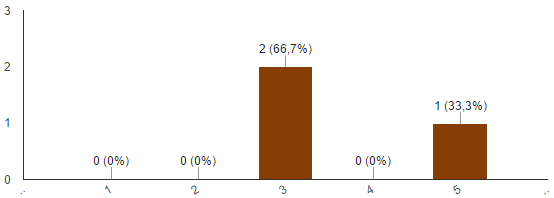
\includegraphics[width=10cm, frame]{figuras/apendiceB-1-2.png}
%\label{figura:grafico_ava_grupoSemPDTI}
%\caption{Aderência à teoria sobre as razões da ausência de um PDTI}
\end{figure}
\\
\\1.2 - A área de TI da minha instituição possui gestores que dominam técnicas e conceitos de nível estratégico na área (Governança de TI). (Escala de 1 a 5, onde 1 indica "discordo totalmente" e 5 "concordo totalmente").
\\Resultado:
\begin{figure}[h]
\centering % para centralizarmos a figura
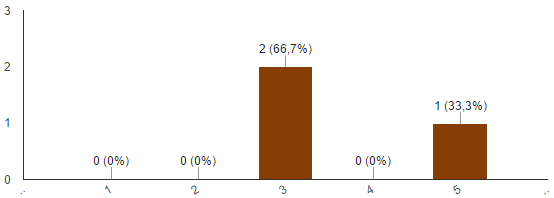
\includegraphics[width=10cm, frame]{figuras/apendiceB-1-2.png}
\end{figure}

\textit{A questão a seguir avalia a aderência da teoria fundamentada nos dados para as instituições sem PDTI:}
\\
\\1.3 - Uma instituição com baixo nível de maturidade em gestão não dá a devida importância à planos estratégicos e não reconhece a TI como parte estratégica da instituição. A área de TI, por sua vez, apresenta deficiências estratégicas como (a) baixo nível de influência da TI na instituição como um todo e (b) equipe inadequada em quantidade e em domínio de técnicas de planejamento; tais fatores (fator “a” e fator “b”) impedem ou dificultam a elaboração do Plano Diretor de TI.
\\Resultado (Escala de 1 a 5, onde 1 indica "discordo totalmente" e 5 "concordo totalmente"):
\begin{figure}[h]
\centering % para centralizarmos a figura
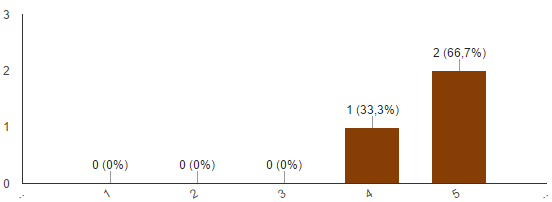
\includegraphics[width=10cm, frame]{figuras/grafico_ava_grupoSemPDTI.PNG}
\end{figure}

\textit{As perguntas a seguir foram destinadas ao grupo que respondeu "não" na questão 1:}
\\
\\2.1 - A participação dos setores, ou seja, das áreas de negócio no PDTI da minha instituição ocorreu com comprometimento e envolvimento satisfatórios. (Escala de 1 a 5, onde 1 indica "discordo totalmente" e 5 "concordo totalmente").
\\Resultado:
\begin{figure}[h]
\centering % para centralizarmos a figura
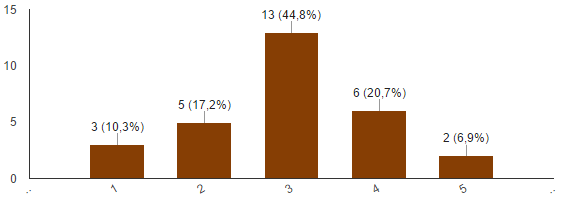
\includegraphics[width=10cm, frame]{figuras/apendiceB-2-1.png}
\end{figure}

\textit{A questão a seguir avalia a aderência da teoria fundamentada nos dados para as instituições sem PDTI:}
\\
\\2.2 - Uma determinada instituição apresenta o seguinte cenário: (a) possui membros que colocam interesses particulares e políticos acima dos interesses da instituição; (b) não possui a percepção de que a TI é parte estratégica e (c) não possuem recursos humanos devidamente capacitados para promover a cultura do planejamento. O efeito causado por (a), (b) e (c) no PDTI da instituição é a "falta de comprometimento e a participação insatisfatória das áreas de negócio" na composição do planejamento de TI. Esta atuação deficiente das áreas de negócio é o principal fator das dificuldades e deficiências encontradas na elaboração de um PDTI.
\\Resultado (Escala de 1 a 5, onde 1 indica "discordo totalmente" e 5 "concordo totalmente"):
\begin{figure}[h]
\centering % para centralizarmos a figura
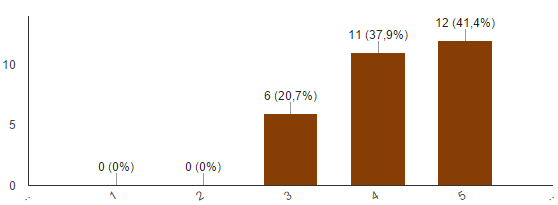
\includegraphics[width=10cm, frame]{figuras/grafico_ava_grupoComPDTI.PNG}
\end{figure} %Questionário e Resuldados de Avaliação
% ---
\chapter{Relatório quantitativo} %Apêndice C
\label{apendice:c_relat_quantitativo}

Este apêndice apresenta um relatório composto dos resultados das questões objetivas do questionário de coleta de dados.
\section{Quanto ao perfil dos respondentes}
Em um total de 53 participantes, o gráfico abaixo apresenta a proporção dos cargos efetivos dos servidores participantes da coleta de dados.

\begin{figure}[h]
\centering % para centralizarmos a figura
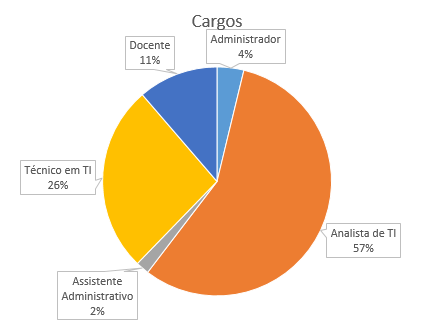
\includegraphics[width=9cm]{figuras/apendiceC_cargos.png}
%\caption{Cargos dos respondentes.}
\end{figure}

Dos 53 participantes, 34 possuem cargo de confiança.

Com relação ao tempo na instituição (em anos), os participantes se distribuem da seguinte forma:
\begin{itemize}
\item 2 anos ou menos: 9 participantes;
\item 3 a 5 anos: 22 participantes;
\item 6 a 10 anos: 14 participantes;
\item 10 a 20 anos: 5 participantes;
\item 20 anos ou mais: 3 participantes.
\end{itemize}

Com relação à formação acadêmica, os participantes estão distribuídos da seguinte forma:
\begin{figure}[h]
\centering % para centralizarmos a figura
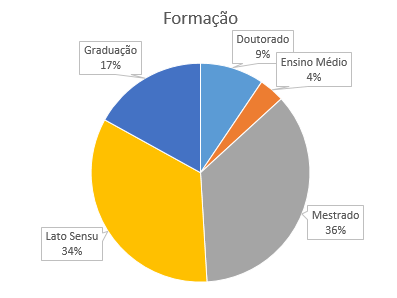
\includegraphics[width=9cm]{figuras/apendiceC_formacao.png}
%\caption{Formação dos respondentes.}
\end{figure}

\section{Quanto ao PDTI}
\begin{itemize}
\item Afirmaram possuir PDTI: 81\% (30 instituições)
\item Afirmaram não possuir PDTI: 19\% (7 instituições)
\end{itemize}

Este resultado se difere dos números do TCU em seu levantamento com 355 órgãos federais \cite{tcu:14}, dos quais 33\% afirmaram não possuir PDTI. Esta diferença sugere que no caso específico de instituições de ensino federais o nível de aderência ao planejamento de TI é melhor do que o percentual geral envolvendo os demais órgãos federais. Porém, é importante ter cautela ao tirar conclusões. Um estudo focado em comparar as instituições de ensino com as demais instituições federais poderia esclarecer as razões desta diferença.

%Foi possível extrair uma visão quantitativa das dificuldades encontradas pelos respondentes que participaram da elaboração do PDTI das suas respectivas instituições. 
No questionário foi perguntado acerca do grau de dificuldade na realização de algumas atividades essenciais no planejamento de TI, o grau de dificuldade poderia variar de 0 (nenhuma dificuldade) a 10 (muita dificuldade). Na figura abaixo é possível inferir que as maiores dificuldades na fase de levantamento de necessidades estão nas atividades de identificação das necessidades de informação e, principalmente, na definição de critérios de priorização das necessidades levantadas. 
\begin{figure}[h]
\centering % para centralizarmos a figura
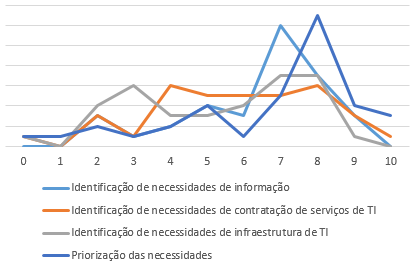
\includegraphics[width=9cm]{figuras/grafico_dificuldades.png}
%\caption{Formação dos respondentes.}
\end{figure}

Foi perguntado para os respondentes do grupo de instituições que possui PDTI se eles seguiram o Guia do SISP (modelo de elaboração do PDTI). Os números absolutos são distribuídos como segue:
\begin{itemize}
\item Não usaram o Guia do SISP: 3 participantes;
\item Usaram o Guia do SISP parcialmente: 12 participantes;
\item Usaram o Guia do SISP completamente: 21 participantes;
\item Não souberam informar: 1 participante.
\end{itemize}

Utilizando a escala de 1 a 5, onde 1 corresponde à "discordo totalmente" e 5 à "concordo totalmente", foi perguntado aos participantes se eles concordam que no PDTI das suas respectivas instituições havia determinados elementos. O gráfico abaixo apresenta a percepção dos participantes sobre a presença destes elementos no PDTI.

\begin{figure}[h]
\centering % para centralizarmos a figura
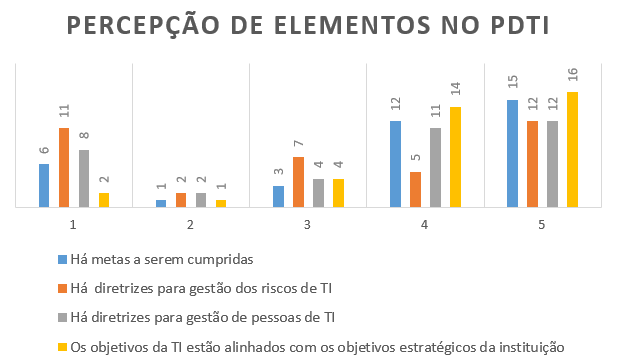
\includegraphics[width=11cm]{figuras/apendiceC_percepcaoelementos.png}
%\caption{Formação dos respondentes.}
\end{figure}
 %Relatório quantitativo
% ---
%\begin{landscape}
\chapter{Respostas dissertativas} %Apêndice D
\label{apendice:d_respostas_disserta}

\section{Respostas do Grupo 1 (sem PDTI)}
A página a seguir contém, na íntegra, as respostas coletadas com participantes de instituições que não possuem PDTI. Estas respostas foram as entradas para a análise de dados com \textit{Grounded Theory}.
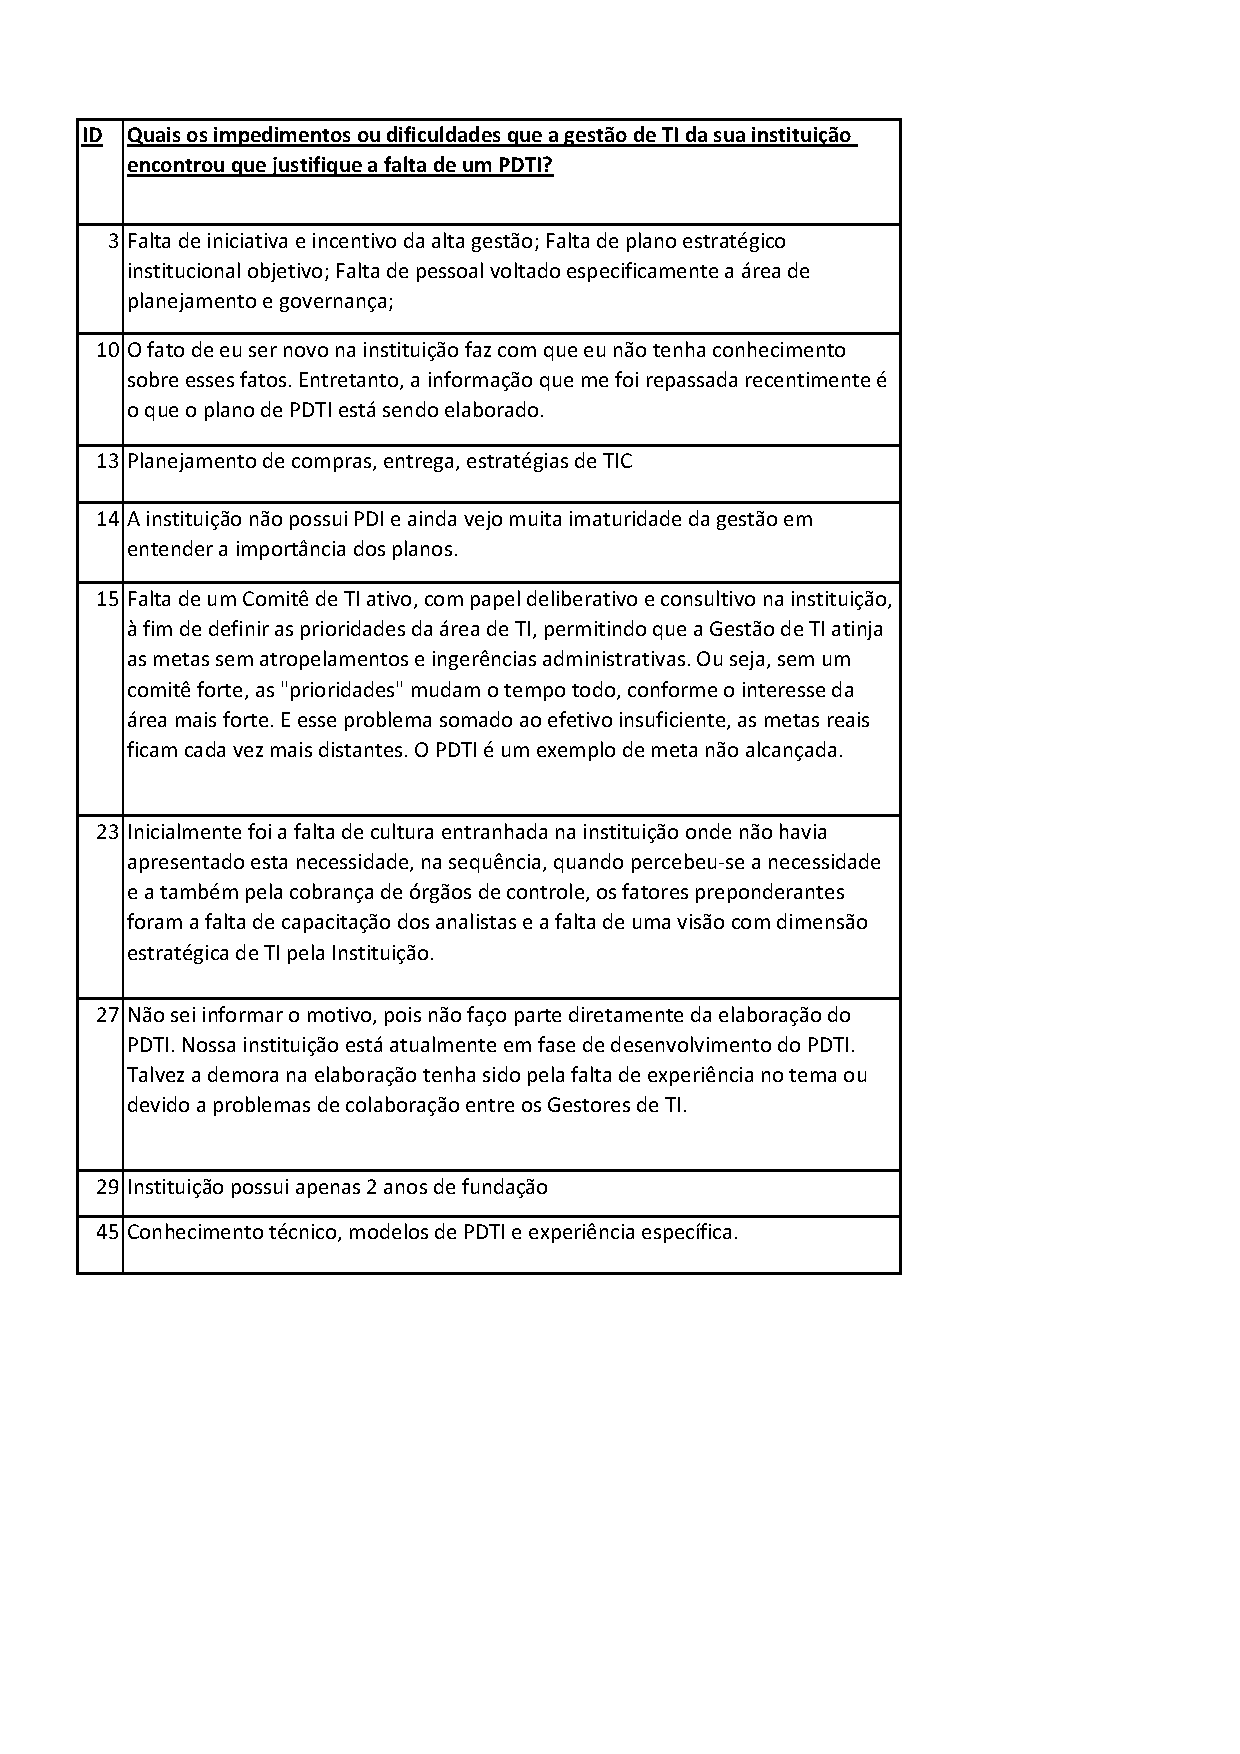
\includepdf[pages=-]{includes/Qualitativas_SEM_PDTI.pdf}

\section{Respostas do Grupo 2 (com PDTI)}
As páginas a seguir contém, na íntegra, as respostas coletadas com participantes de instituições que possuem PDTI. Estas respostas foram as entradas para a análise de dados com \textit{Grounded Theory}.
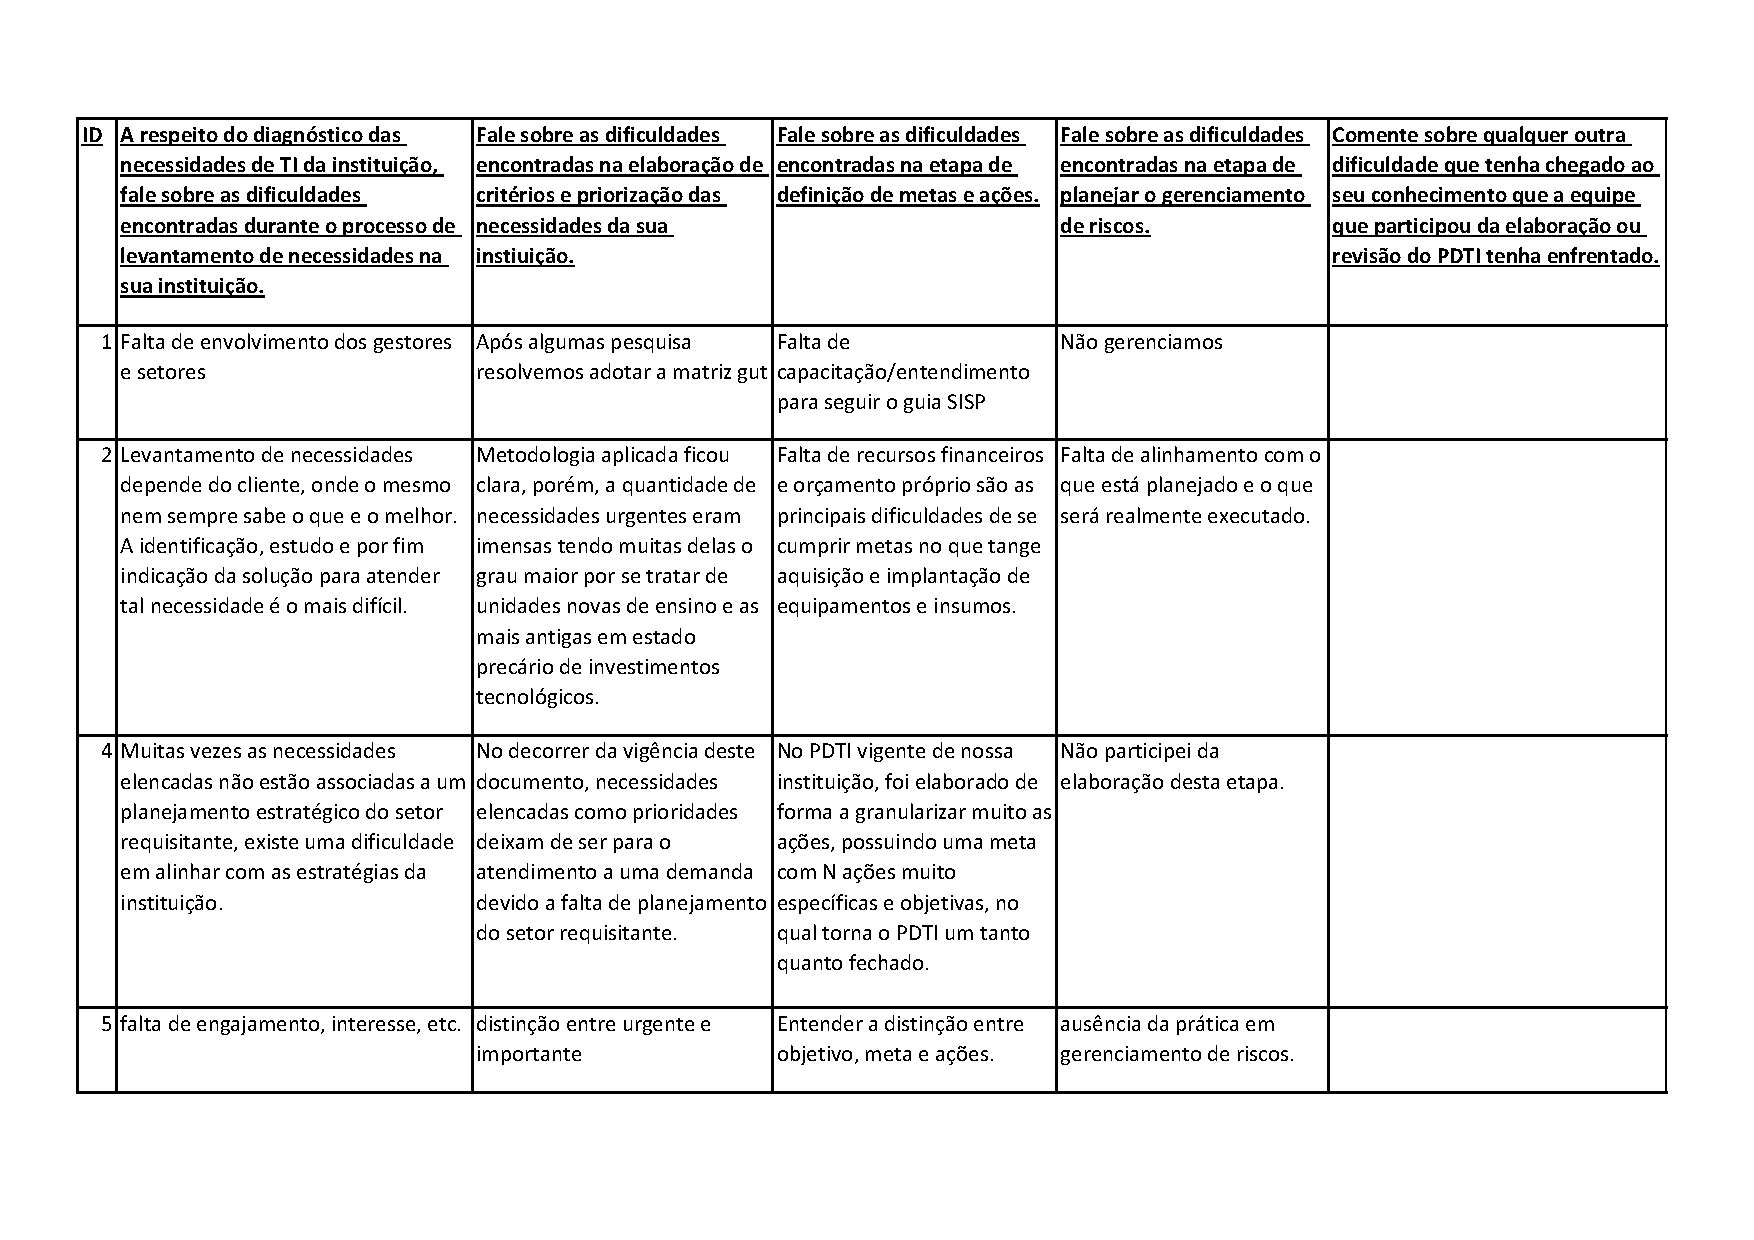
\includepdf[pages=-]{includes/Qualitativas_COM_PDTI.pdf}
 %Respostas dissertativas
% ---
%\end{landscape}
\chapter{Códigos extraídos das respostas} %Anexo E (lista os códigos e os comentários de cada um)
\label{apendice:e_codigos}
\section{Códigos do Grupo 1 (sem PDTI)}
As páginas a seguir compõem o relatório de códigos mapeados no grupo 1. Totalizando 18 códigos, o relatório apresenta a definição de cada código, comentários, além de propriedades e dimensões dos códigos do tipo categoria.

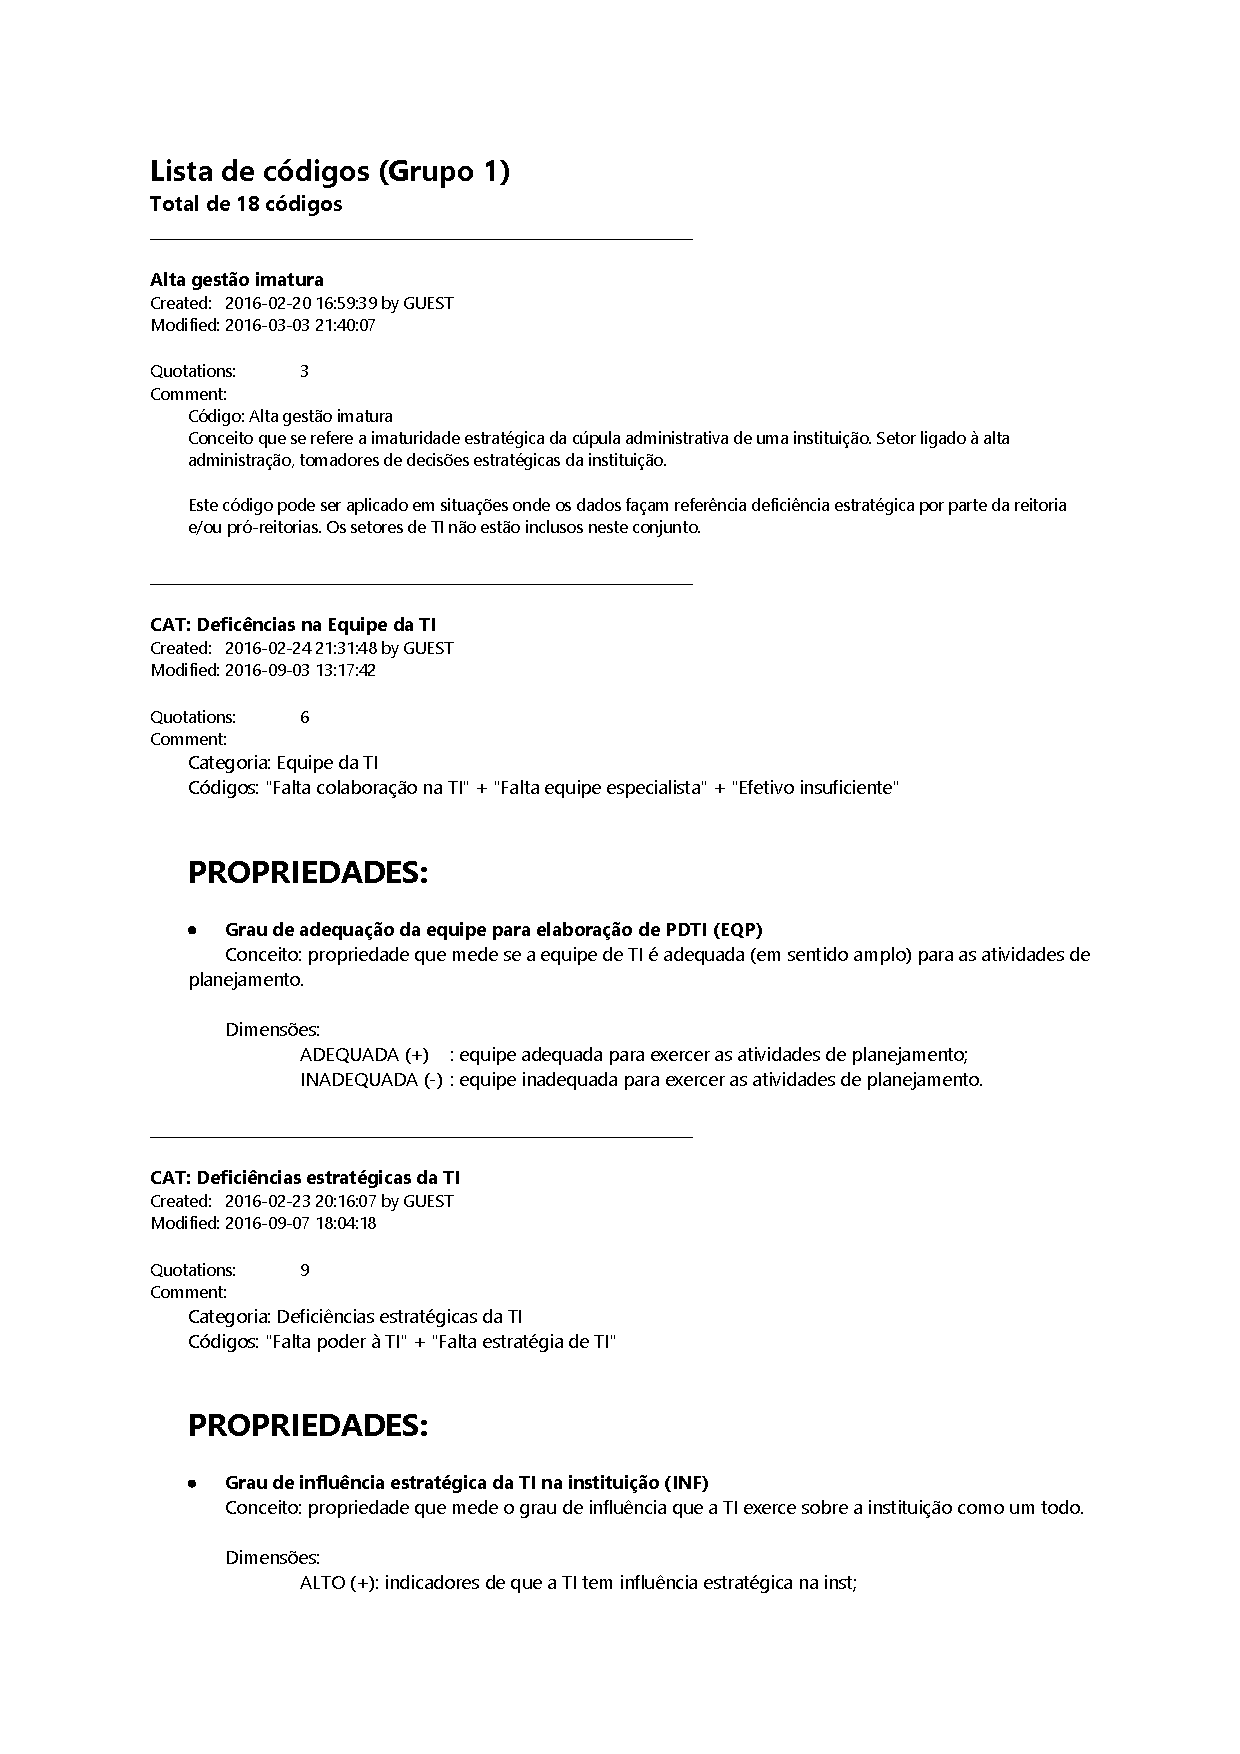
\includepdf[pages=-]{includes/apendiceE_codigos_g1.pdf}


\section{Citações por código do Grupo 1}
As páginas a seguir contém um relatório completo dos 18 códigos mapeados no grupo 1. O relatório apresenta cada citação vinculada a cada código, ou seja, cada trecho das respostas dos participantes que originou determinado código. Além disso, o relatório apresenta os códigos que possuem relacionamento entre si.

\includepdf[pages=-]{includes/apendiceE_codigos_e_citacoes_g1.pdf}


\section{Códigos do Grupo 2 (com PDTI)}
As páginas a seguir compõem o relatório de códigos mapeados no grupo 2. Totalizando 75 códigos, o relatório apresenta a definição de cada código, comentários, além de propriedades e dimensões dos códigos do tipo categoria.

\includepdf[pages=-]{includes/apendiceE_codigos_g2.pdf}


\section{Citações por código do Grupo 2}
As páginas a seguir contém um relatório completo dos 75 códigos mapeados no grupo 2. O relatório apresenta cada citação vinculada a cada código, ou seja, cada trecho das respostas dos participantes que originou determinado código. Além disso, o relatório apresenta os códigos que possuem relacionamento entre si.

\includepdf[pages=-]{includes/apendiceE_codigos_e_citacoes_g2.pdf} %Códigos extraídos das respostas
% ---
\chapter{Notas de microanálise (MA)} %Anexo F (lista as notas MA e seus respectivos conteúdos)
\label{apendice:f_notas_ma}
\section{Notas de microanálise do Grupo 1 (sem PDTI)}
As páginas a seguir contém as 6 notas do tipo MA criadas durante o desenvolvimento da pesquisa sobre o grupo 1.

\includepdf[pages=-]{includes/apendiceF_MA_g1.pdf}

\section{Notas de microanálise do Grupo 2 (com PDTI)}
As páginas a seguir contém as 14 notas do tipo MA criadas durante o desenvolvimento da pesquisa sobre o grupo 2.

\includepdf[pages=-]{includes/apendiceF_MA_g2.pdf} %Notas MA
% ---
%\include{apendiceG} abortei o apêndice G pois as categorias já estão listadadas no apêndice E.
% ---
\chapter{Notas de codificação aberta (OC)} %Anexo H (novo G) (lista as notas OC e seus respectivos conteúdos)
\label{apendice:h_notas_oc}
\section{Notas de codificação aberta do Grupo 1 (sem PDTI)}
As páginas a seguir contém as 6 notas do tipo OC criadas durante o desenvolvimento da pesquisa sobre o grupo 1.

\includepdf[pages=-]{includes/apendiceH_novo_G_OC_g1.pdf}

\section{Notas de codificação aberta do Grupo 2 (com PDTI)}
As páginas a seguir contém as 19 notas do tipo OC criadas durante o desenvolvimento da pesquisa sobre o grupo 2.

\includepdf[pages=-]{includes/apendiceH_novo_G_OC_g2.pdf} %que na verdade é o novo apêndice G: lista as notas OC e seus respectivos conteúdos
% ---
\chapter{Notas de codificação axial (AC)} %Anexo I (lista as notas AC e seus respectivos conteúdos)
\label{apendice:i_notas_ac}
\section{Notas de codificação axial do Grupo 1 (sem PDTI)}
As páginas a seguir contém as 20 notas do tipo AC criadas durante o desenvolvimento da pesquisa sobre o grupo 1.

\includepdf[pages=-]{includes/apendiceI_novo_H_AC_g1.pdf}

\section{Notas de codificação axial do Grupo 2 (com PDTI)}
As páginas a seguir contém as 29 notas do tipo AC criadas durante o desenvolvimento da pesquisa sobre o grupo 2.

\includepdf[pages=-]{includes/apendiceI_novo_H_AC_g2.pdf} %que na verdade é o novo apêndice H: lista as notas AC e seus respectivos conteúdos
% ---
\chapter{Notas de codificação axial - Processos de planejamento de TI} %Anexo J (Etapa de descoberta de processos vinculados aos elementos da teoria)
\label{apendice:j_notas_ac}
\section{Notas de codificação axial do Grupo 1 (sem PDTI)}
As páginas a seguir contém as 6 notas do tipo AC criadas durante o desenvolvimento da pesquisa sobre o grupo 1.

\includepdf[pages=-]{includes/memos_AC_etapa2_grupo1.pdf}

\section{Notas de codificação axial do Grupo 2 (com PDTI)}
As páginas a seguir contém as 8 notas do tipo AC criadas durante o desenvolvimento da pesquisa sobre o grupo 2.

\includepdf[pages=-]{includes/memos_AC_etapa2_grupo2.pdf}

\end{apendicesenv}
% ---


% ----------------------------------------------------------
% Anexos
% ----------------------------------------------------------

% ---
% Inicia os anexos
% ---
%\begin{anexosenv}

% Imprime uma página indicando o início dos anexos
%\partanexos

% ---
%\chapter{exempli} %Anexo H (lista as notas OC e seus respectivos conteúdos)


%\end{anexosenv}

%---------------------------------------------------------------------
% INDICE REMISSIVO
%---------------------------------------------------------------------
\phantompart
\printindex
%---------------------------------------------------------------------

\end{document}
